\documentclass[a4paper,10pt,titlepage]{article}

\usepackage{geometry}
\usepackage{amsmath}
\usepackage{amssymb}
\usepackage{txfonts}
\usepackage{microtype}
\usepackage{epsfig}
\usepackage{graphicx}
\usepackage{moreverb}
\usepackage{hyperref}
\usepackage{listings}
\usepackage{xcolor}
\usepackage{textcomp}
\definecolor{listinggray}{gray}{0.98}
\definecolor{lbcolor}{rgb}{0.98,0.98,0.98}
\lstset{
	backgroundcolor=\color{lbcolor},
	tabsize=4,
	rulecolor=,
	language=matlab,
    basicstyle=\scriptsize\ttfamily,
    upquote=true,
    aboveskip={1.5\baselineskip},
    columns=fixed,
    showstringspaces=false,
    extendedchars=true,
    breaklines=true,
    prebreak = \raisebox{0ex}[0ex][0ex]{\ensuremath{\hookleftarrow}},
    frame=single,
    showtabs=false,
    showspaces=false,
    showstringspaces=false,
    identifierstyle=\ttfamily,
    keywordstyle=\color[rgb]{0,0,1},
    commentstyle=\color[rgb]{0.133,0.545,0.133},
    stringstyle=\color[rgb]{0.627,0.126,0.941},
}
\usepackage{eso-pic}
\usepackage{ifthen}

\AddToShipoutPictureBG{\ifthenelse{\equal{\value{page}}{0}}{}{
\includegraphics{template_files/backgroundlines}}}


\usepackage{tikz}
\usepackage{pgfplots}
\usepackage{tikzscale}
\usepackage{graphicx}
\usepackage{float}
\usepackage{subcaption}
\usepackage{comment}
\usepackage{units}
\usetikzlibrary{external}\tikzexternalize


\title{H1a: Classical scattering by a central potential}
\author{Victor Nilsson and Simon Nilsson}
\date{\today}

\begin{document}

\newgeometry{top=2cm,bottom=2cm,left=2cm,right=2cm}

\begin{titlepage}

\setcounter{page}{0}

\begin{center}
{\huge \bf \color{red} NB: The graded, first version of the report must be
                           returned if you hand in a second time! } \\
\vspace{3cm}
\makeatletter
{ \huge \@title } \\
\vspace{1cm}
{ \Large \@author }\\
\vspace{1cm}
{ \Large \@date }\\
\makeatother
\end{center}

\vfill

\begin{flushright}
{\Large
\begin{tabular}{|c|c|c|}
\hline
Task N\textsuperscript{\underline{o}} & Points & Avail.\ points \\ \hline
\hspace{3cm} & \hspace{3cm} & \hspace{3cm} \\ \hline
~ & ~ & ~ \\ \hline
~ & ~ & ~ \\ \hline
~ & ~ & ~ \\ \hline
~ & ~ & ~ \\ \hline
~ & ~ & ~ \\ \hline
~ & ~ & ~ \\ \hline
~ & ~ & ~ \\ \hline
$\sum$ & ~ & ~ \\
\hline
\end{tabular}}
\end{flushright}

\end{titlepage}

\newgeometry{top=2cm,bottom=2cm,left=1.5cm,right=7.4cm}


\section*{Introduction}

Molecular dynamics is a simulation of the movement of atoms and molecules. What is of interest in such a simulations is e.g. the trajectories of the atoms given specific surrounding parameters such as temperature, pressure, crystal formation etc. For this homeproblem we study the dynamics of aluminium atoms in a FCC crystal lattice.

\section*{Problem 1}

\begin{figure}[H]
    \centering
    \captionsetup[subfigure]{justification=centering}
    \begin{subfigure}[b]{0.40\textwidth}
        \centering
        \resizebox{\columnwidth}{!}{% This file was created by matlab2tikz.
%
%The latest updates can be retrieved from
%  http://www.mathworks.com/matlabcentral/fileexchange/22022-matlab2tikz-matlab2tikz
%where you can also make suggestions and rate matlab2tikz.
%
\definecolor{mycolor1}{rgb}{0.00000,0.44700,0.74100}%
\definecolor{mycolor2}{rgb}{0.85000,0.32500,0.09800}%
\definecolor{mycolor3}{rgb}{0.92900,0.69400,0.12500}%
%
\begin{tikzpicture}

\begin{axis}[%
width=4.521in,
height=3.566in,
at={(0.758in,0.481in)},
scale only axis,
xmin=0,
xmax=100,
xlabel={Time / [ASU]},
ymin=-500000000,
ymax=3000000000,
ylabel={Energy / [ASU]},
axis background/.style={fill=white},
title style={font=\bfseries},
title={Awesome title},
legend style={legend cell align=left,align=left,draw=white!15!black}
]
\addplot [color=mycolor1,solid]
  table[row sep=crcr]{%
0	-857.0284\\
0.1	24095.5953\\
0.2	368482.8188\\
0.3	1345138.0751\\
0.4	2290709.7434\\
0.5	4028094.6967\\
0.6	5098138.1067\\
0.7	5828281.2084\\
0.8	6567207.687\\
0.9	7858390.8086\\
1	9842270.9262\\
1.1	12588912.0788\\
1.2	13906521.2805\\
1.3	14363649.6421\\
1.4	15127580.1113\\
1.5	16948566.4579\\
1.6	17909643.987\\
1.7	20367468.1138\\
1.8	22869417.5343\\
1.9	25193878.986\\
2	28342826.4527\\
2.1	28839450.3935\\
2.2	30331130.3247\\
2.3	32527871.7289\\
2.4	34634700.0354\\
2.5	35313003.6665\\
2.6	38613194.3993\\
2.7	48638010.5486\\
2.8	50151638.1548\\
2.9	52594947.3467\\
3	54230397.1507\\
3.1	55551364.0393\\
3.2	56353883.5097\\
3.3	56770473.197\\
3.4	57220501.7233\\
3.5	58584395.3641\\
3.6	60569094.7586\\
3.7	62692067.526\\
3.8	64324208.0889\\
3.9	65762722.5297\\
4	67438763.6942\\
4.1	69552209.7533\\
4.2	70430322.4085\\
4.3	71847176.2897\\
4.4	73325428.205\\
4.5	75173440.891\\
4.6	76403186.4331\\
4.7	78042735.9443\\
4.8	80436309.9774\\
4.9	81020332.2789\\
5	81313509.7819\\
5.1	82973294.789\\
5.2	85802275.0114\\
5.3	88124809.1011\\
5.4	89401665.4643\\
5.5	91378296.6361\\
5.6	94524164.1069\\
5.7	96460820.7844\\
5.8	99448900.6369\\
5.9	101522748.3995\\
6	102529727.8694\\
6.1	103489313.3208\\
6.2	104609660.0967\\
6.3	105365082.4452\\
6.4	105532086.5228\\
6.5	106508943.8725\\
6.6	108344488.3803\\
6.7	110121709.8413\\
6.8	111763183.3774\\
6.9	113233765.0356\\
7	116169073.1049\\
7.1	118104490.6391\\
7.2	119355631.6227\\
7.3	121436893.1461\\
7.4	125414597.4194\\
7.5	126664833.7799\\
7.6	127860903.3605\\
7.7	128494359.1918\\
7.8	131509667.0702\\
7.9	132868415.0923\\
8	135953076.5134\\
8.1	137422666.2762\\
8.2	139361879.1531\\
8.3	141303725.8262\\
8.4	142346542.104\\
8.5	142517633.7039\\
8.6	144270108.2869\\
8.7	145170602.0524\\
8.8	145451627.1261\\
8.9	147643891.664\\
9	151447749.2793\\
9.1	152875540.1467\\
9.2	153359136.4177\\
9.3	156236432.0684\\
9.4	162088141.3522\\
9.5	163921802.1429\\
9.6	165654966.0414\\
9.7	169058975.3003\\
9.8	171540103.7872\\
9.9	172046015.0507\\
10	172736806.8247\\
10.1	173685307.5643\\
10.2	175732714.4342\\
10.3	183295170.1968\\
10.4	200797840.3644\\
10.5	201756614.886\\
10.6	202525726.5692\\
10.7	203422576.5659\\
10.8	203624812.4169\\
10.9	205182760.1219\\
11	207087252.9362\\
11.1	208871185.2308\\
11.2	210006366.1458\\
11.3	210255337.3167\\
11.4	210892225.7987\\
11.5	211806782.2698\\
11.6	212371310.8326\\
11.7	211843505.3813\\
11.8	211416643.4093\\
11.9	212026648.1661\\
12	214093501.2604\\
12.1	216844292.7644\\
12.2	217815810.938\\
12.3	221439033.8285\\
12.4	225262649.954\\
12.5	225909529.3479\\
12.6	236861155.3667\\
12.7	275089737.4125\\
12.8	275934219.2462\\
12.9	277004785.0409\\
13	279092318.4577\\
13.1	280791193.7368\\
13.2	282402272.2673\\
13.3	283471815.5033\\
13.4	283847235.4979\\
13.5	284676749.7207\\
13.6	286699415.3881\\
13.7	289321199.1244\\
13.8	289394353.1631\\
13.9	288548264.4833\\
14	288333036.0154\\
14.1	290495916.6402\\
14.2	293607656.5212\\
14.3	293674332.2067\\
14.4	293411859.06\\
14.5	294030063.2744\\
14.6	295972105.0342\\
14.7	298374422.487\\
14.8	298514850.4058\\
14.9	299809775.5186\\
15	301295545.5831\\
15.1	301679837.5417\\
15.2	301860737.5009\\
15.3	303144766.5294\\
15.4	302825554.9364\\
15.5	304036624.4536\\
15.6	306718791.1735\\
15.7	308355795.3564\\
15.8	309576938.3408\\
15.9	310345230.2321\\
16	311016053.1378\\
16.1	312132047.8506\\
16.2	312627741.0367\\
16.3	311755558.0128\\
16.4	320523105.8083\\
16.5	320510118.3786\\
16.6	323311961.732\\
16.7	330599491.7075\\
16.8	332636466.8764\\
16.9	339348531.9854\\
17	341513488.8474\\
17.1	348059683.4214\\
17.2	358403752.4416\\
17.3	359870723.2124\\
17.4	360714889.1072\\
17.5	361480827.9965\\
17.6	363364939.7069\\
17.7	363760352.8321\\
17.8	364060902.6576\\
17.9	369031431.9849\\
18	381228445.3508\\
18.1	383351806.6154\\
18.2	388212224.3701\\
18.3	388988339.4032\\
18.4	391771464.5376\\
18.5	394362065.1893\\
18.6	395646513.8304\\
18.7	397945075.0721\\
18.8	398553259.5309\\
18.9	398321093.9276\\
19	400935192.1199\\
19.1	402946871.2045\\
19.2	403766205.1315\\
19.3	405453707.4409\\
19.4	407301724.8853\\
19.5	409720817.2219\\
19.6	416568717.5284\\
19.7	424105779.7432\\
19.8	425676240.9535\\
19.9	427654736.783\\
20	429356679.8849\\
20.1	431715546.8356\\
20.2	434805900.0159\\
20.3	437406645.8773\\
20.4	437919276.065\\
20.5	438375024.8556\\
20.6	438841242.6693\\
20.7	442556269.4132\\
20.8	443977557.2853\\
20.9	446017862.1335\\
21	451845473.2756\\
21.1	456739353.0559\\
21.2	456658388.8079\\
21.3	457840365.3658\\
21.4	459058450.6133\\
21.5	458423564.0334\\
21.6	457393070.5846\\
21.7	456942850.7216\\
21.8	461463687.0176\\
21.9	471061340.7374\\
22	477202160.4461\\
22.1	478705123.4672\\
22.2	488435615.8222\\
22.3	521134981.0696\\
22.4	525049019.8306\\
22.5	525474981.6925\\
22.6	525181723.6958\\
22.7	526417843.8027\\
22.8	527317635.2691\\
22.9	525803314.7795\\
23	525764500.8714\\
23.1	527336477.7655\\
23.2	529916180.0102\\
23.3	534508518.1266\\
23.4	537383594.8652\\
23.5	537774918.8335\\
23.6	539073024.5557\\
23.7	542718243.4654\\
23.8	544188970.7669\\
23.9	545942054.7526\\
24	548359291.4185\\
24.1	554984302.5747\\
24.2	570380538.2067\\
24.3	574466807.6143\\
24.4	577988845.9245\\
24.5	578011702.5423\\
24.6	578411579.2878\\
24.7	584428220.5503\\
24.8	590404924.9629\\
24.9	592073848.1824\\
25	596574298.5346\\
25.1	598317854.493\\
25.2	599923718.9772\\
25.3	602991148.2013\\
25.4	609029281.9493\\
25.5	610031740.62\\
25.6	611783496.9415\\
25.7	614356030.7938\\
25.8	619762472.5001\\
25.9	621313001.1378\\
26	626824961.0616\\
26.1	631028428.1747\\
26.2	632975536.4658\\
26.3	637317503.4272\\
26.4	636857881.1961\\
26.5	640885312.7721\\
26.6	655547155.7677\\
26.7	656108625.5827\\
26.8	660550256.6189\\
26.9	670945302.9953\\
27	672082068.7472\\
27.1	672337396.2293\\
27.2	671588972.3386\\
27.3	674636400.8144\\
27.4	689615127.006\\
27.5	690628514.6705\\
27.6	691288078.0049\\
27.7	694490135.2191\\
27.8	696457350.5842\\
27.9	698949610.3248\\
28	701081983.0886\\
28.1	701110476.7211\\
28.2	701327930.5326\\
28.3	706913668.0548\\
28.4	712393100.5709\\
28.5	713844809.6817\\
28.6	716711771.8375\\
28.7	733503045.282\\
28.8	772833419.3031\\
28.9	771801807.2403\\
29	773249530.5513\\
29.1	775772936.9942\\
29.2	775875972.0667\\
29.3	776131906.6816\\
29.4	776892489.8246\\
29.5	778718693.8248\\
29.6	782384381.4187\\
29.7	783736132.0822\\
29.8	784526552.9683\\
29.9	797055720.9875\\
30	828863502.7653\\
30.1	832206763.1577\\
30.2	836010140.576\\
30.3	839251587.7727\\
30.4	840305339.1744\\
30.5	840682339.2226\\
30.6	843107040.3349\\
30.7	843385574.657\\
30.8	850170535.9814\\
30.9	860510453.4279\\
31	864409603.9424\\
31.1	865876117.8453\\
31.2	867386709.6148\\
31.3	869203327.748\\
31.4	871660151.9729\\
31.5	872530483.7138\\
31.6	871793126.0492\\
31.7	872529825.1074\\
31.8	877423351.038\\
31.9	879501291.4968\\
32	884453700.0664\\
32.1	890333747.4335\\
32.2	892744598.2947\\
32.3	892568006.1555\\
32.4	892965184.5267\\
32.5	895343971.8646\\
32.6	897992503.3279\\
32.7	908114588.1794\\
32.8	925772853.2226\\
32.9	933854707.6963\\
33	949296104.0365\\
33.1	955990115.2917\\
33.2	980614635.9956\\
33.3	982956699.6002\\
33.4	983319565.2633\\
33.5	986299351.8147\\
33.6	992092337.6188\\
33.7	991302294.2488\\
33.8	991762740.7527\\
33.9	993054676.6995\\
34	993696786.4112\\
34.1	1001540458.5562\\
34.2	1015023931.4902\\
34.3	1015780728.1515\\
34.4	1016751732.9899\\
34.5	1019171647.4592\\
34.6	1022140667.5181\\
34.7	1022564790.1363\\
34.8	1023121233.6162\\
34.9	1024806163.2327\\
35	1028785406.0861\\
35.1	1032874669.3947\\
35.2	1037902989.3754\\
35.3	1046999064.6373\\
35.4	1064123329.8069\\
35.5	1071087316.5087\\
35.6	1075257695.2999\\
35.7	1081634225.8557\\
35.8	1081537325.4367\\
35.9	1081490625.2059\\
36	1082733629.2658\\
36.1	1085170346.9647\\
36.2	1085906372.6815\\
36.3	1086549615.8606\\
36.4	1088138541.4471\\
36.5	1088233421.2993\\
36.6	1088943423.4032\\
36.7	1089245190.3235\\
36.8	1089039622.9145\\
36.9	1091880696.7371\\
37	1095410000.5298\\
37.1	1098402579.7476\\
37.2	1104354511.817\\
37.3	1117948195.279\\
37.4	1116979530.3162\\
37.5	1123491614.956\\
37.6	1129826667.4575\\
37.7	1127242691.2529\\
37.8	1126277576.0817\\
37.9	1127917017.3167\\
38	1129778620.1831\\
38.1	1132234809.5226\\
38.2	1130428043.9069\\
38.3	1130496227.3817\\
38.4	1131174434.0119\\
38.5	1131264677.5964\\
38.6	1130486941.4946\\
38.7	1127698748.6321\\
38.8	1128346731.9458\\
38.9	1131207661.5838\\
39	1141213078.9854\\
39.1	1144948798.7074\\
39.2	1148742653.1097\\
39.3	1156374927.7691\\
39.4	1167012101.9759\\
39.5	1169185376.6521\\
39.6	1168393917.0665\\
39.7	1171038776.8607\\
39.8	1181978944.4663\\
39.9	1186827991.0393\\
40	1185727429.7074\\
40.1	1189182735.0074\\
40.2	1195278690.2982\\
40.3	1196886524.4249\\
40.4	1198648024.67\\
40.5	1192796864.775\\
40.6	1194533946.9225\\
40.7	1197305763.4108\\
40.8	1199186418.4767\\
40.9	1198366068.7345\\
41	1197631024.4088\\
41.1	1198619882.67\\
41.2	1200638965.4908\\
41.3	1200729070.0593\\
41.4	1201487189.6697\\
41.5	1203977473.9469\\
41.6	1206406568.1025\\
41.7	1210202362.2478\\
41.8	1213299184.6702\\
41.9	1212344590.2116\\
42	1215113236.2315\\
42.1	1215191825.4085\\
42.2	1216120725.3947\\
42.3	1218305612.3715\\
42.4	1219545917.3518\\
42.5	1219974041.1196\\
42.6	1225819202.712\\
42.7	1238988956.5514\\
42.8	1241912797.8186\\
42.9	1244002905.1901\\
43	1243897355.8998\\
43.1	1243362306.2283\\
43.2	1242351055.3611\\
43.3	1244611985.3436\\
43.4	1248910405.6713\\
43.5	1251826949.749\\
43.6	1256472603.5017\\
43.7	1262531021.5702\\
43.8	1266729073.6775\\
43.9	1269107209.485\\
44	1271268898.1432\\
44.1	1274033405.3749\\
44.2	1275725984.3999\\
44.3	1274935965.3726\\
44.4	1277750788.7505\\
44.5	1279049902.8241\\
44.6	1279731645.9033\\
44.7	1282409681.6605\\
44.8	1288971626.2074\\
44.9	1296112957.6328\\
45	1306311802.2639\\
45.1	1306897043.9519\\
45.2	1308305152.5801\\
45.3	1308825768.5881\\
45.4	1309664897.3785\\
45.5	1310650990.2206\\
45.6	1312144672.6092\\
45.7	1311907227.3521\\
45.8	1311878248.857\\
45.9	1312294749.7377\\
46	1314506323.6148\\
46.1	1319556658.1277\\
46.2	1316967424.7274\\
46.3	1316987108.8967\\
46.4	1315940881.7247\\
46.5	1314444362.637\\
46.6	1315499997.7259\\
46.7	1315409004.103\\
46.8	1314508259.6215\\
46.9	1312090102.5915\\
47	1311962730.6328\\
47.1	1313805624.704\\
47.2	1316683052.7597\\
47.3	1312551715.4708\\
47.4	1313508016.3639\\
47.5	1311186891.996\\
47.6	1311092266.0061\\
47.7	1311549870.5431\\
47.8	1310248024.0236\\
47.9	1312142260.9733\\
48	1314713527.7055\\
48.1	1313999488.5716\\
48.2	1314652622.6918\\
48.3	1319787940.6103\\
48.4	1321506241.1643\\
48.5	1322547862.3009\\
48.6	1325398673.2799\\
48.7	1325871192.1294\\
48.8	1326012716.1465\\
48.9	1327923115.2179\\
49	1328454457.0001\\
49.1	1331951614.497\\
49.2	1337515103.1719\\
49.3	1337928896.5122\\
49.4	1340476160.5973\\
49.5	1344285019.8106\\
49.6	1346677004.0363\\
49.7	1350677681.9634\\
49.8	1352534760.33\\
49.9	1355737396.0907\\
50	1358506912.3453\\
50.1	1361089515.5233\\
50.2	1367286016.499\\
50.3	1370310724.5288\\
50.4	1370444119.9211\\
50.5	1372131811.6979\\
50.6	1374299860.6575\\
50.7	1376566877.0535\\
50.8	1376057202.834\\
50.9	1374983351.6992\\
51	1372916186.0439\\
51.1	1372282905.2523\\
51.2	1373979585.2589\\
51.3	1376785609.1131\\
51.4	1380074831.4843\\
51.5	1381372875.1168\\
51.6	1379776062.2553\\
51.7	1380415047.6136\\
51.8	1388955414.5982\\
51.9	1393510674.645\\
52	1397852387.5043\\
52.1	1396184032.1842\\
52.2	1396140507.7996\\
52.3	1400861719.1963\\
52.4	1402922048.3966\\
52.5	1405428127.3913\\
52.6	1408371775.7299\\
52.7	1411840610.0701\\
52.8	1413871343.9289\\
52.9	1414359854.588\\
53	1414450117.1929\\
53.1	1417937604.4933\\
53.2	1420662194.9537\\
53.3	1421263226.0935\\
53.4	1423513029.7296\\
53.5	1428353715.775\\
53.6	1434627586.5977\\
53.7	1437403939.1629\\
53.8	1439344967.0444\\
53.9	1438601600.2968\\
54	1437946555.9644\\
54.1	1438516371.9432\\
54.2	1444208033.5085\\
54.3	1450451803.7732\\
54.4	1450900280.3903\\
54.5	1456747364.0809\\
54.6	1469253633.6896\\
54.7	1475079729.293\\
54.8	1476689827.7538\\
54.9	1479544382.5388\\
55	1477743310.4021\\
55.1	1476858897.7627\\
55.2	1478991578.2506\\
55.3	1480889509.7309\\
55.4	1483293000.1857\\
55.5	1486630151.5665\\
55.6	1487906523.5372\\
55.7	1490092851.8804\\
55.8	1492800231.5284\\
55.9	1496897967.4567\\
56	1503447022.234\\
56.1	1510886324.5957\\
56.2	1515183534.6352\\
56.3	1515684323.2082\\
56.4	1530421868.5792\\
56.5	1526182007.037\\
56.6	1534658709.8211\\
56.7	1535475889.8426\\
56.8	1541542492.7064\\
56.9	1547079000.1211\\
57	1548295552.814\\
57.1	1548977612.2583\\
57.2	1550517853.3667\\
57.3	1551567178.0123\\
57.4	1544415794.2953\\
57.5	1537995008.0477\\
57.6	1536248653.3148\\
57.7	1537554615.6633\\
57.8	1541162988.5994\\
57.9	1541257172.7403\\
58	1539860591.511\\
58.1	1541696881.3501\\
58.2	1540714835.7386\\
58.3	1543763790.9764\\
58.4	1546414356.4385\\
58.5	1548996991.9442\\
58.6	1548506763.7937\\
58.7	1548671008.6344\\
58.8	1551001122.2898\\
58.9	1554247429.9202\\
59	1556755475.2099\\
59.1	1558813759.8915\\
59.2	1558719716.0389\\
59.3	1557569666.0419\\
59.4	1560291380.2985\\
59.5	1563815177.649\\
59.6	1561257314.3897\\
59.7	1561727147.6682\\
59.8	1564100843.9501\\
59.9	1564587019.8964\\
60	1567084133.0583\\
60.1	1570006783.2394\\
60.2	1571853985.0856\\
60.3	1574024327.6358\\
60.4	1579612594.9361\\
60.5	1584022132.4276\\
60.6	1583149544.9859\\
60.7	1591504915.7737\\
60.8	1603202057.7673\\
60.9	1602037555.3889\\
61	1604509829.757\\
61.1	1605798508.587\\
61.2	1604865004.826\\
61.3	1604001667.8196\\
61.4	1604406063.5145\\
61.5	1606526755.6253\\
61.6	1599173580.0047\\
61.7	1608972379.3194\\
61.8	1607949752.9882\\
61.9	1609001590.2422\\
62	1611049024.0355\\
62.1	1610769991.5533\\
62.2	1618388204.7204\\
62.3	1630058140.5457\\
62.4	1634027790.8576\\
62.5	1637746198.1754\\
62.6	1640729532.5749\\
62.7	1643588402.1267\\
62.8	1648205186.1575\\
62.9	1650716427.2161\\
63	1649484764.3946\\
63.1	1647460595.6766\\
63.2	1649475669.4122\\
63.3	1650836844.2628\\
63.4	1656676435.5714\\
63.5	1652085303.9649\\
63.6	1645068372.3408\\
63.7	1641750946.1122\\
63.8	1642898536.6467\\
63.9	1644777481.4389\\
64	1643831061.1389\\
64.1	1637509100.3363\\
64.2	1639954745.7417\\
64.3	1642545817.3164\\
64.4	1643777305.6185\\
64.5	1649052047.8071\\
64.6	1648758501.8872\\
64.7	1647202533.0142\\
64.8	1646086494.2279\\
64.9	1645301065.1324\\
65	1643518394.7243\\
65.1	1646983044.4075\\
65.2	1644522953.7125\\
65.3	1640736757.7926\\
65.4	1640789416.2161\\
65.5	1651678603.7729\\
65.6	1665133849.2297\\
65.7	1665875072.9505\\
65.8	1664834175.6125\\
65.9	1666196728.8044\\
66	1673395631.6711\\
66.1	1682481219.9649\\
66.2	1685683257.3731\\
66.3	1687475995.58\\
66.4	1689294625.5502\\
66.5	1690480936.1731\\
66.6	1689785241.8723\\
66.7	1692005246.3614\\
66.8	1697801921.4298\\
66.9	1700409752.3069\\
67	1707822413.3719\\
67.1	1720961738.8101\\
67.2	1725543641.7828\\
67.3	1728367246.4533\\
67.4	1729825154.5918\\
67.5	1731921791.8515\\
67.6	1739397315.4896\\
67.7	1746004680.2339\\
67.8	1753909409.6571\\
67.9	1767317968.1157\\
68	1774404754.5251\\
68.1	1773425377.3414\\
68.2	1774115264.6113\\
68.3	1777219017.164\\
68.4	1784591530.6052\\
68.5	1792052895.1885\\
68.6	1793513549.8149\\
68.7	1795373826.1081\\
68.8	1798869428.2401\\
68.9	1804217881.6912\\
69	1805114086.6037\\
69.1	1808517665.3892\\
69.2	1810823114.0657\\
69.3	1810891588.445\\
69.4	1809285962.3625\\
69.5	1810562232.5757\\
69.6	1814092611.5244\\
69.7	1814147450.4025\\
69.8	1818905920.875\\
69.9	1823922463.6926\\
70	1830286157.5843\\
70.1	1834876575.1751\\
70.2	1833906903.7975\\
70.3	1836045605.9891\\
70.4	1840951420.4946\\
70.5	1843905307.5169\\
70.6	1841454580.6111\\
70.7	1840562427.6949\\
70.8	1841658293.4687\\
70.9	1846466521.8144\\
71	1845780592.5896\\
71.1	1844106467.8787\\
71.2	1844117895.7581\\
71.3	1846042458.6235\\
71.4	1846226978.1287\\
71.5	1845858767.6191\\
71.6	1848015224.1116\\
71.7	1848937448.1653\\
71.8	1850183424.5598\\
71.9	1850945907.3649\\
72	1852761174.5429\\
72.1	1856033024.1775\\
72.2	1854944088.7283\\
72.3	1855192689.4453\\
72.4	1855415407.363\\
72.5	1855520608.5626\\
72.6	1855334487.5862\\
72.7	1857856031.4503\\
72.8	1861959653.0525\\
72.9	1865181942.2578\\
73	1863292849.768\\
73.1	1870472196.9098\\
73.2	1885442582.0068\\
73.3	1886427694.4611\\
73.4	1889659075.0368\\
73.5	1892850018.1758\\
73.6	1888945659.4234\\
73.7	1888740997.5047\\
73.8	1891715634.3958\\
73.9	1893194068.7043\\
74	1893856538.8091\\
74.1	1892293977.8561\\
74.2	1889609832.9644\\
74.3	1890922919.3732\\
74.4	1892544500.9575\\
74.5	1897331996.7435\\
74.6	1906119244.2767\\
74.7	1908247083.6038\\
74.8	1908458736.6136\\
74.9	1910545419.3166\\
75	1917496251.0133\\
75.1	1926696380.9182\\
75.2	1930920933.6591\\
75.3	1936547014.0836\\
75.4	1940007644.0649\\
75.5	1944059548.8681\\
75.6	1943986203.3649\\
75.7	1944134788.2432\\
75.8	1946803298.5569\\
75.9	1945479553.0443\\
76	1942811686.9705\\
76.1	1943213454.2021\\
76.2	1942576773.5806\\
76.3	1942816517.6378\\
76.4	1945954979.8581\\
76.5	1950048285.5243\\
76.6	1958580937.2508\\
76.7	1966087290.7549\\
76.8	1969489753.8198\\
76.9	1969848494.7049\\
77	1966988521.8671\\
77.1	1965679292.747\\
77.2	1968865294.9065\\
77.3	1970871744.9747\\
77.4	1977831886.0646\\
77.5	1982025659.3659\\
77.6	1981616171.3528\\
77.7	1979169189.5795\\
77.8	1980806881.2203\\
77.9	1981896094.4707\\
78	1981150322.4186\\
78.1	1981800765.7552\\
78.2	1982735524.4444\\
78.3	1982754407.2451\\
78.4	1982470816.9742\\
78.5	1985451673.7237\\
78.6	1988495947.7035\\
78.7	1989918424.7671\\
78.8	1989188477.7972\\
78.9	1987948173.6701\\
79	1992454027.4466\\
79.1	1999294664.9269\\
79.2	2006035052.8997\\
79.3	2020081690.9604\\
79.4	2021551875.7604\\
79.5	2022935809.5872\\
79.6	2024699096.5097\\
79.7	2025001472.889\\
79.8	2023076182.1583\\
79.9	2030568785.8913\\
80	2041752520.8657\\
80.1	2040351509.5251\\
80.2	2042983086.797\\
80.3	2046898440.9229\\
80.4	2044500054.9103\\
80.5	2041141109.99\\
80.6	2041698806.0314\\
80.7	2044850644.2062\\
80.8	2042698908.355\\
80.9	2039896243.5281\\
81	2037658153.6513\\
81.1	2036465289.0906\\
81.2	2039541252.3019\\
81.3	2043696710.0186\\
81.4	2043276699.1607\\
81.5	2044725575.592\\
81.6	2048606675.2547\\
81.7	2049071006.3786\\
81.8	2048137872.9761\\
81.9	2043923412.1441\\
82	2042831194.9546\\
82.1	2041065895.3898\\
82.2	2040774504.834\\
82.3	2043756921.8946\\
82.4	2042570979.5684\\
82.5	2043948713.9059\\
82.6	2045755375.8652\\
82.7	2045923198.0926\\
82.8	2047161665.9772\\
82.9	2045211874.0124\\
83	2040081213.5504\\
83.1	2040636768.0139\\
83.2	2043099401.639\\
83.3	2045478915.5034\\
83.4	2048461416.1856\\
83.5	2050879071.4479\\
83.6	2052658484.967\\
83.7	2054476910.3055\\
83.8	2056008560.416\\
83.9	2058044639.0081\\
84	2057283279.7193\\
84.1	2055288367.9109\\
84.2	2055251597.2935\\
84.3	2056893600.1729\\
84.4	2058031736.4433\\
84.5	2060305776.9766\\
84.6	2060992945.7848\\
84.7	2059191712.7549\\
84.8	2060091308.7848\\
84.9	2064847179.9934\\
85	2065164733.1657\\
85.1	2066931059.1557\\
85.2	2073450170.0216\\
85.3	2075757910.9707\\
85.4	2078991518.614\\
85.5	2086538643.3015\\
85.6	2088810276.1318\\
85.7	2090695152.2586\\
85.8	2088377410.6648\\
85.9	2090870684.1265\\
86	2096158853.9069\\
86.1	2102326796.9347\\
86.2	2104127203.6353\\
86.3	2099208391.0837\\
86.4	2103703327.422\\
86.5	2105398137.6703\\
86.6	2107216620.3532\\
86.7	2108018305.8731\\
86.8	2104903671.5649\\
86.9	2103605989.7349\\
87	2108213898.1034\\
87.1	2113475070.1552\\
87.2	2114108843.513\\
87.3	2120425823.7671\\
87.4	2126059141.5792\\
87.5	2122526207.9867\\
87.6	2121213543.0533\\
87.7	2122162819.5219\\
87.8	2124868208.0462\\
87.9	2135504152.2251\\
88	2140714743.45\\
88.1	2138161348.9777\\
88.2	2138860851.7837\\
88.3	2142290040.7915\\
88.4	2138548140.5887\\
88.5	2137930170.4841\\
88.6	2142263610.7945\\
88.7	2148706922.2026\\
88.8	2153717290.4605\\
88.9	2155688957.3963\\
89	2186426103.3062\\
89.1	2255848590.8376\\
89.2	2256569837.8611\\
89.3	2248656774.0002\\
89.4	2242207301.4437\\
89.5	2244830384.9439\\
89.6	2243653057.9268\\
89.7	2239417211.3556\\
89.8	2237876498.0279\\
89.9	2237668600.4328\\
90	2238172071.8273\\
90.1	2239568659.5222\\
90.2	2241671616.4708\\
90.3	2239866302.7541\\
90.4	2239084892.589\\
90.5	2238944186.2675\\
90.6	2237865891.6053\\
90.7	2240624645.0122\\
90.8	2245822016.0347\\
90.9	2247445402.8937\\
91	2247046090.1738\\
91.1	2251381843.5307\\
91.2	2264213109.6546\\
91.3	2268958912.215\\
91.4	2274240909.022\\
91.5	2277585308.4409\\
91.6	2281812282.3187\\
91.7	2286357363.4844\\
91.8	2288588337.7288\\
91.9	2290228116.8962\\
92	2301631154.6009\\
92.1	2337272629.9255\\
92.2	2332599650.7904\\
92.3	2330639672.5383\\
92.4	2330546795.6919\\
92.5	2330820718.5566\\
92.6	2327525609.9252\\
92.7	2326339155.2578\\
92.8	2334933482.7147\\
92.9	2355444458.8729\\
93	2359491849.2238\\
93.1	2359366681.9672\\
93.2	2362181059.0864\\
93.3	2365303004.539\\
93.4	2372819520.6125\\
93.5	2379927810.3876\\
93.6	2381780271.9991\\
93.7	2385715110.9694\\
93.8	2390900603.8042\\
93.9	2392892988.2466\\
94	2389090656.8036\\
94.1	2387275756.6748\\
94.2	2385726900.281\\
94.3	2382616713.4412\\
94.4	2379724076.2682\\
94.5	2380589573.0291\\
94.6	2384809351.4148\\
94.7	2386513804.8236\\
94.8	2387316574.8983\\
94.9	2392097186.4756\\
95	2394342158.0036\\
95.1	2395661921.6573\\
95.2	2396195773.3245\\
95.3	2396488469.5997\\
95.4	2396079182.0188\\
95.5	2398295100.6444\\
95.6	2403261442.12\\
95.7	2406278970.0452\\
95.8	2410223745.2658\\
95.9	2413997949.8463\\
96	2417192988.0392\\
96.1	2420331432.9727\\
96.2	2429484546.4172\\
96.3	2438413698.6497\\
96.4	2439547707.6858\\
96.5	2438692207.4484\\
96.6	2439318171.1559\\
96.7	2442481475.1183\\
96.8	2443917127.7291\\
96.9	2447237096.3054\\
97	2450379055.586\\
97.1	2455752880.7046\\
97.2	2463421725.768\\
97.3	2468716584.0427\\
97.4	2473394218.3513\\
97.5	2475644416.1858\\
97.6	2475421301.0923\\
97.7	2479615930.9289\\
97.8	2480707742.5339\\
97.9	2479824636.866\\
98	2479124407.4117\\
98.1	2476014830.6727\\
98.2	2474358998.3288\\
98.3	2476628489.6727\\
98.4	2479423235.1316\\
98.5	2483319638.3091\\
98.6	2484557073.1462\\
98.7	2494763505.7914\\
98.8	2512202235.9907\\
98.9	2511083925.2665\\
99	2512385001.1453\\
99.1	2515175978.7071\\
99.2	2519896516.6484\\
99.3	2526145894.8657\\
99.4	2528827832.1583\\
99.5	2531273789.3124\\
99.6	2531410654.3204\\
99.7	2535016865.2887\\
99.8	2522580921.2148\\
99.9	2592106061.8661\\
};
\addlegendentry{Total energy};

\addplot [color=mycolor2,solid]
  table[row sep=crcr]{%
0	-857.0284\\
0.1	-133.2825\\
0.2	2576.5563\\
0.3	2281.3926\\
0.4	2752.7477\\
0.5	2594.4902\\
0.6	1989.902\\
0.7	1856.2758\\
0.8	2670.3686\\
0.9	2521.1948\\
1	2711.3269\\
1.1	2702.3887\\
1.2	2222.4094\\
1.3	1895.6478\\
1.4	2760.4033\\
1.5	1977.6586\\
1.6	2936.1026\\
1.7	2636.902\\
1.8	2542.5431\\
1.9	2568.4542\\
2	2642.5013\\
2.1	2101.5411\\
2.2	2482.1399\\
2.3	2690.3318\\
2.4	1887.1138\\
2.5	2160.667\\
2.6	3435.6702\\
2.7	2517.3828\\
2.8	2840.8781\\
2.9	2508.4154\\
3	2549.2923\\
3.1	1954.4631\\
3.2	1976.2074\\
3.3	2058.327\\
3.4	2419.3428\\
3.5	2583.7818\\
3.6	2497.2806\\
3.7	2727.5677\\
3.8	2018.0071\\
3.9	2338.7138\\
4	2590.1965\\
4.1	2669.299\\
4.2	2603.2727\\
4.3	2228.7105\\
4.4	2925.0473\\
4.5	2226.8022\\
4.6	2720.5287\\
4.7	2734.0307\\
4.8	2344.0141\\
4.9	2498.6158\\
5	2319.0283\\
5.1	2757.7532\\
5.2	2436.3019\\
5.3	2440.45\\
5.4	2153.1431\\
5.5	2449.4314\\
5.6	2750.0143\\
5.7	3178.0237\\
5.8	2619.5416\\
5.9	2409.1643\\
6	2168.5\\
6.1	2218.7701\\
6.2	2344.9023\\
6.3	1823.1828\\
6.4	2506.5739\\
6.5	2334.5655\\
6.6	2802.2436\\
6.7	2597.145\\
6.8	2055.2902\\
6.9	2583.3201\\
7	2877.0557\\
7.1	2302.1299\\
7.2	2337.6708\\
7.3	2812.7387\\
7.4	2670.388\\
7.5	2575.486\\
7.6	2385.416\\
7.7	2773.7285\\
7.8	1827.87\\
7.9	3008.7087\\
8	2348.938\\
8.1	2104.5198\\
8.2	2508.0973\\
8.3	2638.2275\\
8.4	2333.7847\\
8.5	2618.1319\\
8.6	2150.948\\
8.7	2612.5651\\
8.8	2398.8566\\
8.9	2567.571\\
9	2633.1612\\
9.1	2641.1032\\
9.2	2636.8076\\
9.3	3004.0463\\
9.4	2585.6883\\
9.5	2474.264\\
9.6	2527.927\\
9.7	2216.9186\\
9.8	2293.8317\\
9.9	2469.3886\\
10	2224.5888\\
10.1	2931.4828\\
10.2	2617.3429\\
10.3	2959.4956\\
10.4	2759.5183\\
10.5	2514.7843\\
10.6	2706.6276\\
10.7	2249.1643\\
10.8	2573.3541\\
10.9	2226.9087\\
11	2287.5868\\
11.1	2395.121\\
11.2	2039.3587\\
11.3	1970.8763\\
11.4	2262.551\\
11.5	1723.1027\\
11.6	2240.1882\\
11.7	2446.0537\\
11.8	1934.57\\
11.9	2481.1682\\
12	2614.7286\\
12.1	2648.0994\\
12.2	1999.6695\\
12.3	2629.0705\\
12.4	2487.4821\\
12.5	2107.9636\\
12.6	3975.0432\\
12.7	2371.9913\\
12.8	2297.2355\\
12.9	2865.0719\\
13	2540.3668\\
13.1	2292.1583\\
13.2	1926.4242\\
13.3	2061.3916\\
13.4	3025.6736\\
13.5	2762.3162\\
13.6	3001.3668\\
13.7	2578.3007\\
13.8	2296.453\\
13.9	2657.2112\\
14	2617.4945\\
14.1	2738.1555\\
14.2	2041.1622\\
14.3	2584.7228\\
14.4	3036.1019\\
14.5	2533.7327\\
14.6	2603.1436\\
14.7	2620.3555\\
14.8	2614.9338\\
14.9	2163.5346\\
15	2542.981\\
15.1	2327.7708\\
15.2	2778.9173\\
15.3	1919.5084\\
15.4	2422.4056\\
15.5	2734.8021\\
15.6	2609.2352\\
15.7	2299.46\\
15.8	2579.9673\\
15.9	2056.6533\\
16	1995.6017\\
16.1	2359.5028\\
16.2	2024.2216\\
16.3	3366.2327\\
16.4	2049.6949\\
16.5	2549.3654\\
16.6	3193.9206\\
16.7	2709.5838\\
16.8	3113.7107\\
16.9	2450.9856\\
17	2758.3732\\
17.1	3199.8095\\
17.2	2328.7952\\
17.3	2211.8868\\
17.4	2424.046\\
17.5	2641.6388\\
17.6	2420.9898\\
17.7	2622.9501\\
17.8	2370.7863\\
17.9	2708.5073\\
18	2457.8207\\
18.1	3210.1768\\
18.2	2076.5251\\
18.3	2192.1093\\
18.4	2407.7809\\
18.5	2294.0654\\
18.6	2266.4117\\
18.7	2026.6481\\
18.8	2835.6632\\
18.9	2624.0071\\
19	2551.6331\\
19.1	3050.4186\\
19.2	2393.8602\\
19.3	2655.1456\\
19.4	2300.8517\\
19.5	2314.1108\\
19.6	3012.8755\\
19.7	2285.4557\\
19.8	2460.8719\\
19.9	2307.8748\\
20	2944.2872\\
20.1	2576.067\\
20.2	2807.78\\
20.3	2473.284\\
20.4	2052.1989\\
20.5	2537.0949\\
20.6	3453.8635\\
20.7	2461.376\\
20.8	2167.3255\\
20.9	2554.4274\\
21	2610.5935\\
21.1	2131.2183\\
21.2	2325.2927\\
21.3	2434.2203\\
21.4	2548.448\\
21.5	1881.9144\\
21.6	2209.9735\\
21.7	2854.3342\\
21.8	2753.0658\\
21.9	3331.822\\
22	2530.408\\
22.1	2443.7413\\
22.2	3843.7529\\
22.3	3218.5336\\
22.4	2630.0758\\
22.5	2178.9362\\
22.6	2152.6628\\
22.7	2381.9493\\
22.8	2283.0295\\
22.9	2096.9607\\
23	2250.1247\\
23.1	2641.9042\\
23.2	3058.6302\\
23.3	2238.1462\\
23.4	2261.9824\\
23.5	2913.7582\\
23.6	2644.5575\\
23.7	2577.4434\\
23.8	2670.6911\\
23.9	2890.5759\\
24	1699.9347\\
24.1	3758.5186\\
24.2	2196.5972\\
24.3	2868.4904\\
24.4	2366.3985\\
24.5	1896.7284\\
24.6	2539.7214\\
24.7	3179.7968\\
24.8	2009.2106\\
24.9	3098.8898\\
25	2650.1076\\
25.1	2098.6224\\
25.2	2579.5121\\
25.3	2807.9432\\
25.4	2168.9133\\
25.5	2169.2697\\
25.6	2980.5486\\
25.7	2787.5689\\
25.8	1780.5103\\
25.9	3281.5761\\
26	2539.7689\\
26.1	2000.9159\\
26.2	3101.9406\\
26.3	2367.3129\\
26.4	2309.3584\\
26.5	3582.597\\
26.6	2507.676\\
26.7	2826.9261\\
26.8	3398.602\\
26.9	2220.7881\\
27	2213.8377\\
27.1	2413.2348\\
27.2	2362.8716\\
27.3	3315.7763\\
27.4	2979.1235\\
27.5	2525.5892\\
27.6	3160.6176\\
27.7	2396.0558\\
27.8	2614.7922\\
27.9	2531.9669\\
28	1854.8989\\
28.1	2166.7784\\
28.2	2079.8877\\
28.3	2781.1753\\
28.4	2543.1752\\
28.5	3097.6558\\
28.6	2195.7115\\
28.7	3668.0379\\
28.8	2645.0743\\
28.9	2330.5885\\
29	2661.8528\\
29.1	2280.7531\\
29.2	2595.5264\\
29.3	2300.8238\\
29.4	2081.2465\\
29.5	2562.2499\\
29.6	2050.1701\\
29.7	2491.0785\\
29.8	1786.5721\\
29.9	3202.259\\
30	2331.1036\\
30.1	2528.889\\
30.2	2637.9541\\
30.3	2328.2885\\
30.4	1832.7392\\
30.5	2313.6308\\
30.6	2107.2776\\
30.7	2733.0278\\
30.8	2861.8578\\
30.9	2277.4522\\
31	2510.3305\\
31.1	1996.3267\\
31.2	2331.3744\\
31.3	2464.748\\
31.4	2507.8015\\
31.5	2266.9371\\
31.6	3334.3624\\
31.7	3038.6189\\
31.8	2645.3265\\
31.9	2535.3271\\
32	2908.9916\\
32.1	2462.1889\\
32.2	2460.4297\\
32.3	1980.8614\\
32.4	2441.9125\\
32.5	2181.2269\\
32.6	2921.7252\\
32.7	3242.7542\\
32.8	1994.8382\\
32.9	3262.1558\\
33	2739.3475\\
33.1	3629.5389\\
33.2	2174.4726\\
33.3	2341.1536\\
33.4	2666.8943\\
33.5	2715.6804\\
33.6	2512.9207\\
33.7	2900.6259\\
33.8	2259.3263\\
33.9	2327.6115\\
34	2283.1563\\
34.1	2789.5721\\
34.2	2662.1887\\
34.3	2637.6767\\
34.4	2449.0674\\
34.5	2055.0811\\
34.6	2087.8138\\
34.7	3030.1046\\
34.8	2966.0863\\
34.9	2886.8971\\
35	2456.1212\\
35.1	2094.3165\\
35.2	3143.9017\\
35.3	3166.5932\\
35.4	2751.3242\\
35.5	2277.958\\
35.6	2700.7382\\
35.7	2009.9651\\
35.8	2623.8659\\
35.9	2355.1408\\
36	2104.0688\\
36.1	2817.4705\\
36.2	2211.3884\\
36.3	2519.7951\\
36.4	2522.0382\\
36.5	2138.5962\\
36.6	2348.6256\\
36.7	2200.5045\\
36.8	2630.558\\
36.9	1973.4607\\
37	2678.2087\\
37.1	2467.9751\\
37.2	2768.6769\\
37.3	2415.257\\
37.4	2780.4158\\
37.5	3243.9821\\
37.6	2437.0262\\
37.7	2387.0437\\
37.8	2810.8749\\
37.9	2020.057\\
38	2578.655\\
38.1	2125.5747\\
38.2	2495.2278\\
38.3	2413.9006\\
38.4	2607.4702\\
38.5	2287.5415\\
38.6	1975.506\\
38.7	2680.2338\\
38.8	2263.0992\\
38.9	2655.0753\\
39	2279.6457\\
39.1	2789.2465\\
39.2	3421.2422\\
39.3	3074.3496\\
39.4	2430.182\\
39.5	2592.6556\\
39.6	2429.713\\
39.7	2895.8417\\
39.8	2737.2421\\
39.9	1589.2373\\
40	2482.5476\\
40.1	2895.2259\\
40.2	2464.0945\\
40.3	2201.7066\\
40.4	2150.9709\\
40.5	3537.7584\\
40.6	2815.6817\\
40.7	2103.5072\\
40.8	2400.5215\\
40.9	2465.6406\\
41	2416.4203\\
41.1	2344.7888\\
41.2	2382.7903\\
41.3	2215.7876\\
41.4	2765.9183\\
41.5	2688.8625\\
41.6	2413.697\\
41.7	2355.7802\\
41.8	2678.673\\
41.9	2200.7516\\
42	2554.1944\\
42.1	2523.5657\\
42.2	2020.9564\\
42.3	2592.522\\
42.4	2251.1181\\
42.5	2612.1299\\
42.6	3105.3396\\
42.7	2611.3589\\
42.8	2052.1451\\
42.9	2540.1117\\
43	2763.7475\\
43.1	2288.9629\\
43.2	2851.5808\\
43.3	2520.7487\\
43.4	1961.1845\\
43.5	2380.1866\\
43.6	2214.5901\\
43.7	2325.7981\\
43.8	2367.0751\\
43.9	2231.1557\\
44	2376.0235\\
44.1	2671.7417\\
44.2	2518.1735\\
44.3	2926.4697\\
44.4	2576.2257\\
44.5	1993.9101\\
44.6	1968.2661\\
44.7	2708.8203\\
44.8	3138.2336\\
44.9	3941.3331\\
45	2465.771\\
45.1	2687.167\\
45.2	2602.7883\\
45.3	2679.0511\\
45.4	2487.8144\\
45.5	1817.3732\\
45.6	2052.4777\\
45.7	2491.3613\\
45.8	2505.8286\\
45.9	2191.8782\\
46	2897.2656\\
46.1	2300.7183\\
46.2	3183.8157\\
46.3	2468.6303\\
46.4	2148.2166\\
46.5	1817.7402\\
46.6	3294.4993\\
46.7	2372.8293\\
46.8	2440.6957\\
46.9	2935.7665\\
47	2310.9111\\
47.1	2534.6578\\
47.2	1949.2985\\
47.3	3240.4871\\
47.4	3031.8422\\
47.5	2170.4483\\
47.6	2930.5387\\
47.7	2420.3813\\
47.8	2830.6622\\
47.9	2385.4327\\
48	2821.2394\\
48.1	2383.333\\
48.2	2591.54\\
48.3	2342.5742\\
48.4	2985.714\\
48.5	3058.1146\\
48.6	2294.2754\\
48.7	1810.996\\
48.8	2210.2184\\
48.9	2121.4795\\
49	2192.8395\\
49.1	2584.4996\\
49.2	2558.0822\\
49.3	2387.7422\\
49.4	2454.5525\\
49.5	2631.102\\
49.6	2543.2736\\
49.7	2389.8003\\
49.8	2655.0379\\
49.9	2612.024\\
50	2478.518\\
50.1	2462.9177\\
50.2	2445.3504\\
50.3	2364.4666\\
50.4	2377.2133\\
50.5	2410.1174\\
50.6	2357.038\\
50.7	2723.1809\\
50.8	2893.4324\\
50.9	2722.3699\\
51	2146.3349\\
51.1	2435.4897\\
51.2	2604.2993\\
51.3	2878.3523\\
51.4	2325.4999\\
51.5	2334.7038\\
51.6	2260.2874\\
51.7	3202.3521\\
51.8	1785.9158\\
51.9	2524.8514\\
52	2291.307\\
52.1	2218.8778\\
52.2	2877.3565\\
52.3	2490.7283\\
52.4	2957.1496\\
52.5	2502.509\\
52.6	2149.8101\\
52.7	2386.0009\\
52.8	2935.464\\
52.9	2559.3515\\
53	2456.1696\\
53.1	2828.6588\\
53.2	2551.8906\\
53.3	2405.4075\\
53.4	2652.5786\\
53.5	2590.2757\\
53.6	2487.7755\\
53.7	2679.4275\\
53.8	2350.6985\\
53.9	2110.741\\
54	2257.5828\\
54.1	2080.9061\\
54.2	3297.3998\\
54.3	2691.7067\\
54.4	2388.9615\\
54.5	3174.2475\\
54.6	2731.3686\\
54.7	2516.5259\\
54.8	3289.4767\\
54.9	1924.9695\\
55	2766.1375\\
55.1	2131.2849\\
55.2	2254.7825\\
55.3	2547.8567\\
55.4	2563.9244\\
55.5	2761.6474\\
55.6	2205.034\\
55.7	2019.7878\\
55.8	2448.9277\\
55.9	2410.4524\\
56	2930.6713\\
56.1	2402.1295\\
56.2	2603.007\\
56.3	3683.3472\\
56.4	2742.6557\\
56.5	3293.4504\\
56.6	2107.8229\\
56.7	2418.8238\\
56.8	2568.8438\\
56.9	2389.0724\\
57	2699.8523\\
57.1	2194.8103\\
57.2	2258.3374\\
57.3	1757.7264\\
57.4	2649.1758\\
57.5	2197.9996\\
57.6	2466.6136\\
57.7	2402.3114\\
57.8	2554.692\\
57.9	2399.8411\\
58	2570.0922\\
58.1	2043.914\\
58.2	2631.2293\\
58.3	2437.7992\\
58.4	3088.4263\\
58.5	2197.4703\\
58.6	1928.0488\\
58.7	2975.3599\\
58.8	2825.9231\\
58.9	3053.4451\\
59	3021.8612\\
59.1	2180.2691\\
59.2	2155.0538\\
59.3	2595.9099\\
59.4	2782.1033\\
59.5	2481.921\\
59.6	2827.9401\\
59.7	3059.0398\\
59.8	2318.9975\\
59.9	2049.8757\\
60	2724.8635\\
60.1	2438.8575\\
60.2	2510.2091\\
60.3	1828.3558\\
60.4	2640.5143\\
60.5	2444.0667\\
60.6	2382.4147\\
60.7	3321.8875\\
60.8	2306.2345\\
60.9	2628.4167\\
61	2388.0738\\
61.1	2394.0151\\
61.2	2600.5308\\
61.3	2080.2166\\
61.4	2965.4227\\
61.5	1697.5533\\
61.6	3374.9548\\
61.7	2456.3509\\
61.8	2448.2461\\
61.9	2051.8876\\
62	2608.3455\\
62.1	2721.5791\\
62.2	2695.3866\\
62.3	2180.7499\\
62.4	2224.5091\\
62.5	2401.6036\\
62.6	2028.4444\\
62.7	2582.7977\\
62.8	2278.8929\\
62.9	2406.5087\\
63	2291.317\\
63.1	2353.7265\\
63.2	2764.4142\\
63.3	3137.0303\\
63.4	2826.8054\\
63.5	2811.7778\\
63.6	2148.0678\\
63.7	1991.1776\\
63.8	1988.2709\\
63.9	2690.0668\\
64	2763.9714\\
64.1	3238.8348\\
64.2	2321.2339\\
64.3	2410.4853\\
64.4	3462.1643\\
64.5	2670.5681\\
64.6	3061.072\\
64.7	2321.4765\\
64.8	1889.9755\\
64.9	2736.8043\\
65	3093.3643\\
65.1	2310.7775\\
65.2	2622.0662\\
65.3	2847.3149\\
65.4	1963.753\\
65.5	2602.6132\\
65.6	1995.036\\
65.7	2582.7904\\
65.8	2724.8618\\
65.9	2190.0175\\
66	2546.007\\
66.1	2203.8672\\
66.2	1951.2329\\
66.3	2873.1848\\
66.4	2303.3274\\
66.5	2249.6535\\
66.6	2893.7605\\
66.7	2518.1425\\
66.8	2535.134\\
66.9	2607.0622\\
67	2502.1677\\
67.1	2571.0766\\
67.2	2167.2162\\
67.3	2350.862\\
67.4	2683.8918\\
67.5	2352.9227\\
67.6	3083.3793\\
67.7	2635.6641\\
67.8	2948.4259\\
67.9	3395.0968\\
68	2602.7572\\
68.1	2772.983\\
68.2	2634.0047\\
68.3	2344.0692\\
68.4	2517.6485\\
68.5	2300.7152\\
68.6	2222.8429\\
68.7	2525.0562\\
68.8	2372.2091\\
68.9	2411.2377\\
69	2120.7751\\
69.1	2660.858\\
69.2	2776.3099\\
69.3	2295.9831\\
69.4	2255.7594\\
69.5	2583.6528\\
69.6	2194.2958\\
69.7	3174.8569\\
69.8	2648.5834\\
69.9	3066.6867\\
70	3153.5028\\
70.1	2478.3617\\
70.2	2808.953\\
70.3	2604.3209\\
70.4	2519.4357\\
70.5	2733.6514\\
70.6	2707.3863\\
70.7	2452.7867\\
70.8	2912.3457\\
70.9	2727.0136\\
71	2784.6839\\
71.1	2103.6782\\
71.2	2759.893\\
71.3	2350.2806\\
71.4	2452.8131\\
71.5	2355.8326\\
71.6	2653.1457\\
71.7	2475.7623\\
71.8	2281.2045\\
71.9	2247.8534\\
72	2120.7296\\
72.1	2230.4123\\
72.2	2771.8493\\
72.3	2564.6939\\
72.4	2610.1254\\
72.5	2355.8365\\
72.6	2596.6458\\
72.7	2196.026\\
72.8	3309.9729\\
72.9	2544.3677\\
73	2569.7705\\
73.1	3500.1095\\
73.2	2449.279\\
73.3	2374.4726\\
73.4	3180.3319\\
73.5	1952.5744\\
73.6	2240.5548\\
73.7	2465.6403\\
73.8	2494.9027\\
73.9	2992.8309\\
74	2459.5598\\
74.1	2673.7318\\
74.2	2591.1902\\
74.3	2231.9743\\
74.4	2742.8586\\
74.5	2664.2062\\
74.6	2556.705\\
74.7	2000.2335\\
74.8	2388.2466\\
74.9	2123.7475\\
75	2860.0508\\
75.1	2523.5709\\
75.2	2462.1591\\
75.3	2261.5001\\
75.4	2311.9977\\
75.5	2530.8879\\
75.6	2465.1132\\
75.7	1960.6278\\
75.8	2274.555\\
75.9	2843.467\\
76	2296.0021\\
76.1	2511.6882\\
76.2	2971.1393\\
76.3	2397.3642\\
76.4	2796.5365\\
76.5	2745.287\\
76.6	2646.0156\\
76.7	2389.9862\\
76.8	2396.617\\
76.9	2666.6877\\
77	2127.6916\\
77.1	2374.2071\\
77.2	2383.4823\\
77.3	3060.4473\\
77.4	2491.1263\\
77.5	2511.5227\\
77.6	1885.2009\\
77.7	2350.8787\\
77.8	2131.5917\\
77.9	2227.6084\\
78	2305.0244\\
78.1	2222.7597\\
78.2	2083.1019\\
78.3	2150.4954\\
78.4	2431.0946\\
78.5	2207.3195\\
78.6	2167.1117\\
78.7	2141.3549\\
78.8	2269.1265\\
78.9	2079.5591\\
79	2795.3816\\
79.1	2015.3326\\
79.2	3037.252\\
79.3	2500.6269\\
79.4	2327.2603\\
79.5	2057.9611\\
79.6	1904.4214\\
79.7	2720.8584\\
79.8	2628.9312\\
79.9	2843.3942\\
80	2175.5364\\
80.1	2285.1624\\
80.2	2836.9847\\
80.3	2556.2064\\
80.4	2454.2943\\
80.5	2235.4612\\
80.6	2799.2866\\
80.7	2230.3975\\
80.8	2561.04\\
80.9	2009.2339\\
81	2400.7348\\
81.1	2612.7831\\
81.2	2465.8285\\
81.3	2820.7192\\
81.4	2163.9828\\
81.5	2504.4184\\
81.6	2684.1497\\
81.7	2335.6844\\
81.8	2138.8463\\
81.9	3099.7564\\
82	2331.3671\\
82.1	2642.9306\\
82.2	2403.6135\\
82.3	2436.0978\\
82.4	2579.0581\\
82.5	2368.2935\\
82.6	2617.8532\\
82.7	1961.6099\\
82.8	2604.2963\\
82.9	2319.5\\
83	2403.643\\
83.1	2278.7727\\
83.2	2284.5214\\
83.3	2536.8937\\
83.4	2873.678\\
83.5	2207.1463\\
83.6	2640.7316\\
83.7	2067.7051\\
83.8	2582.9467\\
83.9	2608.5348\\
84	2532.0562\\
84.1	2654.8971\\
84.2	2788.7378\\
84.3	2544.2547\\
84.4	2295.7431\\
84.5	2793.7958\\
84.6	2560.8413\\
84.7	2582.3933\\
84.8	2934.3363\\
84.9	2469.2885\\
85	2858.9707\\
85.1	2611.7695\\
85.2	2090.1464\\
85.3	2186.5731\\
85.4	2687.1572\\
85.5	2364.6639\\
85.6	2338.8672\\
85.7	2346.337\\
85.8	2890.1017\\
85.9	2387.4615\\
86	2532.2254\\
86.1	2476.4176\\
86.2	2737.0368\\
86.3	3255.4977\\
86.4	2388.8475\\
86.5	2203.3506\\
86.6	2397.7799\\
86.7	2769.6747\\
86.8	2406.4247\\
86.9	2284.4584\\
87	2538.0418\\
87.1	2586.4214\\
87.2	2739.8083\\
87.3	3152.2386\\
87.4	3407.5024\\
87.5	2957.0868\\
87.6	2576.6446\\
87.7	2387.4997\\
87.8	3171.5802\\
87.9	2557.0033\\
88	2023.8203\\
88.1	2113.5004\\
88.2	2009.4529\\
88.3	2358.6432\\
88.4	2352.8598\\
88.5	2383.0657\\
88.6	2001.8521\\
88.7	2291.4812\\
88.8	2389.3471\\
88.9	2444.6248\\
89	3959.8108\\
89.1	2409.1892\\
89.2	2571.8174\\
89.3	2728.402\\
89.4	1892.2453\\
89.5	2702.3309\\
89.6	2261.1952\\
89.7	2498.0326\\
89.8	2140.732\\
89.9	2122.5929\\
90	2204.8992\\
90.1	2821.4051\\
90.2	2526.152\\
90.3	2894.44\\
90.4	2105.0313\\
90.5	2670.7248\\
90.6	1965.7262\\
90.7	2238.0228\\
90.8	2398.5499\\
90.9	2180.0784\\
91	2126.4253\\
91.1	3285.8705\\
91.2	2562.5308\\
91.3	2472.9794\\
91.4	2199.2799\\
91.5	2526.8236\\
91.6	2375.1838\\
91.7	2350.1536\\
91.8	2556.9812\\
91.9	1980.2704\\
92	4719.1901\\
92.1	2933.4546\\
92.2	2165.3249\\
92.3	2788.6201\\
92.4	2704.2438\\
92.5	2280.663\\
92.6	1884.1424\\
92.7	2191.6387\\
92.8	3039.0155\\
92.9	2258.0906\\
93	1946.6326\\
93.1	3049.0742\\
93.2	2505.2489\\
93.3	3072.9934\\
93.4	2741.8917\\
93.5	2350.8586\\
93.6	2315.5244\\
93.7	2129.332\\
93.8	3099.5152\\
93.9	2505.4613\\
94	2358.0177\\
94.1	2331.7999\\
94.2	2608.5162\\
94.3	2631.5408\\
94.4	2340.998\\
94.5	2243.2255\\
94.6	2442.521\\
94.7	2240.8592\\
94.8	2562.0628\\
94.9	2362.1148\\
95	2185.9575\\
95.1	2273.7198\\
95.2	2248.013\\
95.3	1989.6915\\
95.4	2666.9476\\
95.5	2942.4125\\
95.6	2401.8932\\
95.7	2218.7525\\
95.8	2131.2067\\
95.9	2705.0061\\
96	1675.5385\\
96.1	2143.0542\\
96.2	2477.2473\\
96.3	2230.6587\\
96.4	2611.1197\\
96.5	2234.3516\\
96.6	2578.2167\\
96.7	2560.2412\\
96.8	2582.6303\\
96.9	2509.2163\\
97	2391.6994\\
97.1	2574.0616\\
97.2	2078.7788\\
97.3	2740.162\\
97.4	2387.4407\\
97.5	1916.9423\\
97.6	2312.0046\\
97.7	2604.3082\\
97.8	2548.0345\\
97.9	2606.3608\\
98	2369.6807\\
98.1	2548.9752\\
98.2	2101.6394\\
98.3	2181.5208\\
98.4	2434.3797\\
98.5	2169.6727\\
98.6	2211.3396\\
98.7	3196.6253\\
98.8	2836.2252\\
98.9	2623.4341\\
99	2377.8663\\
99.1	2576.0013\\
99.2	2881.9668\\
99.3	2475.5186\\
99.4	2484.8205\\
99.5	2424.5316\\
99.6	3089.3291\\
99.7	2418.2766\\
99.8	4694.522\\
99.9	3373.073\\
};
\addlegendentry{Potential energy};

\addplot [color=mycolor3,solid]
  table[row sep=crcr]{%
0	0\\
0.1	24228.8778\\
0.2	365906.2625\\
0.3	1342856.6825\\
0.4	2287956.9957\\
0.5	4025500.2065\\
0.6	5096148.2047\\
0.7	5826424.9326\\
0.8	6564537.3184\\
0.9	7855869.6138\\
1	9839559.5993\\
1.1	12586209.6901\\
1.2	13904298.8711\\
1.3	14361753.9943\\
1.4	15124819.708\\
1.5	16946588.7993\\
1.6	17906707.8844\\
1.7	20364831.2118\\
1.8	22866874.9912\\
1.9	25191310.5318\\
2	28340183.9514\\
2.1	28837348.8524\\
2.2	30328648.1848\\
2.3	32525181.3971\\
2.4	34632812.9216\\
2.5	35310842.9995\\
2.6	38609758.7291\\
2.7	48635493.1658\\
2.8	50148797.2767\\
2.9	52592438.9313\\
3	54227847.8584\\
3.1	55549409.5762\\
3.2	56351907.3023\\
3.3	56768414.87\\
3.4	57218082.3805\\
3.5	58581811.5823\\
3.6	60566597.478\\
3.7	62689339.9583\\
3.8	64322190.0818\\
3.9	65760383.8159\\
4	67436173.4977\\
4.1	69549540.4543\\
4.2	70427719.1358\\
4.3	71844947.5792\\
4.4	73322503.1577\\
4.5	75171214.0888\\
4.6	76400465.9044\\
4.7	78040001.9136\\
4.8	80433965.9633\\
4.9	81017833.6631\\
5	81311190.7536\\
5.1	82970537.0358\\
5.2	85799838.7095\\
5.3	88122368.6511\\
5.4	89399512.3212\\
5.5	91375847.2047\\
5.6	94521414.0926\\
5.7	96457642.7607\\
5.8	99446281.0953\\
5.9	101520339.2352\\
6	102527559.3694\\
6.1	103487094.5507\\
6.2	104607315.1944\\
6.3	105363259.2624\\
6.4	105529579.9489\\
6.5	106506609.307\\
6.6	108341686.1367\\
6.7	110119112.6963\\
6.8	111761128.0872\\
6.9	113231181.7155\\
7	116166196.0492\\
7.1	118102188.5092\\
7.2	119353293.9519\\
7.3	121434080.4074\\
7.4	125411927.0314\\
7.5	126662258.2939\\
7.6	127858517.9445\\
7.7	128491585.4633\\
7.8	131507839.2002\\
7.9	132865406.3836\\
8	135950727.5754\\
8.1	137420561.7564\\
8.2	139359371.0558\\
8.3	141301087.5987\\
8.4	142344208.3193\\
8.5	142515015.572\\
8.6	144267957.3389\\
8.7	145167989.4873\\
8.8	145449228.2695\\
8.9	147641324.093\\
9	151445116.1181\\
9.1	152872899.0435\\
9.2	153356499.6101\\
9.3	156233428.0221\\
9.4	162085555.6639\\
9.5	163919327.8789\\
9.6	165652438.1144\\
9.7	169056758.3817\\
9.8	171537809.9555\\
9.9	172043545.6621\\
10	172734582.2359\\
10.1	173682376.0815\\
10.2	175730097.0913\\
10.3	183292210.7012\\
10.4	200795080.8461\\
10.5	201754100.1017\\
10.6	202523019.9416\\
10.7	203420327.4016\\
10.8	203622239.0628\\
10.9	205180533.2132\\
11	207084965.3494\\
11.1	208868790.1098\\
11.2	210004326.7871\\
11.3	210253366.4404\\
11.4	210889963.2477\\
11.5	211805059.1671\\
11.6	212369070.6444\\
11.7	211841059.3276\\
11.8	211414708.8393\\
11.9	212024166.9979\\
12	214090886.5318\\
12.1	216841644.665\\
12.2	217813811.2685\\
12.3	221436404.758\\
12.4	225260162.4719\\
12.5	225907421.3843\\
12.6	236857180.3235\\
12.7	275087365.4212\\
12.8	275931922.0107\\
12.9	277001919.969\\
13	279089778.0909\\
13.1	280788901.5785\\
13.2	282400345.8431\\
13.3	283469754.1117\\
13.4	283844209.8243\\
13.5	284673987.4045\\
13.6	286696414.0213\\
13.7	289318620.8237\\
13.8	289392056.7101\\
13.9	288545607.2721\\
14	288330418.5209\\
14.1	290493178.4847\\
14.2	293605615.359\\
14.3	293671747.4839\\
14.4	293408822.9581\\
14.5	294027529.5417\\
14.6	295969501.8906\\
14.7	298371802.1315\\
14.8	298512235.472\\
14.9	299807611.984\\
15	301293002.6021\\
15.1	301677509.7709\\
15.2	301857958.5836\\
15.3	303142847.021\\
15.4	302823132.5308\\
15.5	304033889.6515\\
15.6	306716181.9383\\
15.7	308353495.8964\\
15.8	309574358.3735\\
15.9	310343173.5788\\
16	311014057.5361\\
16.1	312129688.3478\\
16.2	312625716.8151\\
16.3	311752191.7801\\
16.4	320521056.1134\\
16.5	320507569.0132\\
16.6	323308767.8114\\
16.7	330596782.1237\\
16.8	332633353.1657\\
16.9	339346080.9998\\
17	341510730.4742\\
17.1	348056483.6119\\
17.2	358401423.6464\\
17.3	359868511.3256\\
17.4	360712465.0612\\
17.5	361478186.3577\\
17.6	363362518.7171\\
17.7	363757729.882\\
17.8	364058531.8713\\
17.9	369028723.4776\\
18	381225987.5301\\
18.1	383348596.4386\\
18.2	388210147.845\\
18.3	388986147.2939\\
18.4	391769056.7567\\
18.5	394359771.1239\\
18.6	395644247.4187\\
18.7	397943048.424\\
18.8	398550423.8677\\
18.9	398318469.9205\\
19	400932640.4868\\
19.1	402943820.7859\\
19.2	403763811.2713\\
19.3	405451052.2953\\
19.4	407299424.0336\\
19.5	409718503.1111\\
19.6	416565704.6529\\
19.7	424103494.2875\\
19.8	425673780.0816\\
19.9	427652428.9082\\
20	429353735.5977\\
20.1	431712970.7686\\
20.2	434803092.2359\\
20.3	437404172.5933\\
20.4	437917223.8661\\
20.5	438372487.7607\\
20.6	438837788.8058\\
20.7	442553808.0372\\
20.8	443975389.9598\\
20.9	446015307.7061\\
21	451842862.6821\\
21.1	456737221.8376\\
21.2	456656063.5152\\
21.3	457837931.1455\\
21.4	459055902.1653\\
21.5	458421682.119\\
21.6	457390860.6111\\
21.7	456939996.3874\\
21.8	461460933.9518\\
21.9	471058008.9154\\
22	477199630.0381\\
22.1	478702679.7259\\
22.2	488431772.0693\\
22.3	521131762.536\\
22.4	525046389.7548\\
22.5	525472802.7563\\
22.6	525179571.033\\
22.7	526415461.8534\\
22.8	527315352.2396\\
22.9	525801217.8188\\
23	525762250.7467\\
23.1	527333835.8613\\
23.2	529913121.38\\
23.3	534506279.9804\\
23.4	537381332.8828\\
23.5	537772005.0753\\
23.6	539070379.9982\\
23.7	542715666.022\\
23.8	544186300.0758\\
23.9	545939164.1767\\
24	548357591.4838\\
24.1	554980544.0561\\
24.2	570378341.6095\\
24.3	574463939.1239\\
24.4	577986479.526\\
24.5	578009805.8139\\
24.6	578409039.5664\\
24.7	584425040.7535\\
24.8	590402915.7523\\
24.9	592070749.2926\\
25	596571648.427\\
25.1	598315755.8706\\
25.2	599921139.4651\\
25.3	602988340.2581\\
25.4	609027113.036\\
25.5	610029571.3503\\
25.6	611780516.3929\\
25.7	614353243.2249\\
25.8	619760691.9898\\
25.9	621309719.5617\\
26	626822421.2927\\
26.1	631026427.2588\\
26.2	632972434.5252\\
26.3	637315136.1143\\
26.4	636855571.8377\\
26.5	640881730.1751\\
26.6	655544648.0917\\
26.7	656105798.6566\\
26.8	660546858.0169\\
26.9	670943082.2072\\
27	672079854.9095\\
27.1	672334982.9945\\
27.2	671586609.467\\
27.3	674633085.0381\\
27.4	689612147.8825\\
27.5	690625989.0813\\
27.6	691284917.3873\\
27.7	694487739.1633\\
27.8	696454735.792\\
27.9	698947078.3579\\
28	701080128.1897\\
28.1	701108309.9427\\
28.2	701325850.6449\\
28.3	706910886.8795\\
28.4	712390557.3957\\
28.5	713841712.0259\\
28.6	716709576.126\\
28.7	733499377.2441\\
28.8	772830774.2288\\
28.9	771799476.6518\\
29	773246868.6985\\
29.1	775770656.2411\\
29.2	775873376.5403\\
29.3	776129605.8578\\
29.4	776890408.5781\\
29.5	778716131.5749\\
29.6	782382331.2486\\
29.7	783733641.0037\\
29.8	784524766.3962\\
29.9	797052518.7285\\
30	828861171.6617\\
30.1	832204234.2687\\
30.2	836007502.6219\\
30.3	839249259.4842\\
30.4	840303506.4352\\
30.5	840680025.5918\\
30.6	843104933.0573\\
30.7	843382841.6292\\
30.8	850167674.1236\\
30.9	860508175.9757\\
31	864407093.6119\\
31.1	865874121.5186\\
31.2	867384378.2404\\
31.3	869200863\\
31.4	871657644.1714\\
31.5	872528216.7767\\
31.6	871789791.6868\\
31.7	872526786.4885\\
31.8	877420705.7115\\
31.9	879498756.1697\\
32	884450791.0748\\
32.1	890331285.2446\\
32.2	892742137.865\\
32.3	892566025.2941\\
32.4	892962742.6142\\
32.5	895341790.6377\\
32.6	897989581.6027\\
32.7	908111345.4252\\
32.8	925770858.3844\\
32.9	933851445.5405\\
33	949293364.689\\
33.1	955986485.7528\\
33.2	980612461.523\\
33.3	982954358.4466\\
33.4	983316898.369\\
33.5	986296636.1343\\
33.6	992089824.6981\\
33.7	991299393.6229\\
33.8	991760481.4264\\
33.9	993052349.088\\
34	993694503.2549\\
34.1	1001537668.9841\\
34.2	1015021269.3015\\
34.3	1015778090.4748\\
34.4	1016749283.9225\\
34.5	1019169592.3781\\
34.6	1022138579.7043\\
34.7	1022561760.0317\\
34.8	1023118267.5299\\
34.9	1024803276.3356\\
35	1028782949.9649\\
35.1	1032872575.0782\\
35.2	1037899845.4737\\
35.3	1046995898.0441\\
35.4	1064120578.4827\\
35.5	1071085038.5507\\
35.6	1075254994.5617\\
35.7	1081632215.8906\\
35.8	1081534701.5708\\
35.9	1081488270.0651\\
36	1082731525.197\\
36.1	1085167529.4942\\
36.2	1085904161.2931\\
36.3	1086547096.0655\\
36.4	1088136019.4089\\
36.5	1088231282.7031\\
36.6	1088941074.7776\\
36.7	1089242989.819\\
36.8	1089036992.3565\\
36.9	1091878723.2764\\
37	1095407322.3211\\
37.1	1098400111.7725\\
37.2	1104351743.1401\\
37.3	1117945780.022\\
37.4	1116976749.9004\\
37.5	1123488370.9739\\
37.6	1129824230.4313\\
37.7	1127240304.2092\\
37.8	1126274765.2068\\
37.9	1127914997.2597\\
38	1129776041.5281\\
38.1	1132232683.9479\\
38.2	1130425548.6791\\
38.3	1130493813.4811\\
38.4	1131171826.5417\\
38.5	1131262390.0549\\
38.6	1130484965.9886\\
38.7	1127696068.3983\\
38.8	1128344468.8466\\
38.9	1131205006.5085\\
39	1141210799.3397\\
39.1	1144946009.4609\\
39.2	1148739231.8675\\
39.3	1156371853.4195\\
39.4	1167009671.7939\\
39.5	1169182783.9965\\
39.6	1168391487.3535\\
39.7	1171035881.019\\
39.8	1181976207.2242\\
39.9	1186826401.802\\
40	1185724947.1598\\
40.1	1189179839.7815\\
40.2	1195276226.2037\\
40.3	1196884322.7183\\
40.4	1198645873.6991\\
40.5	1192793327.0166\\
40.6	1194531131.2408\\
40.7	1197303659.9036\\
40.8	1199184017.9552\\
40.9	1198363603.0939\\
41	1197628607.9885\\
41.1	1198617537.8812\\
41.2	1200636582.7005\\
41.3	1200726854.2717\\
41.4	1201484423.7514\\
41.5	1203974785.0844\\
41.6	1206404154.4055\\
41.7	1210200006.4676\\
41.8	1213296505.9972\\
41.9	1212342389.46\\
42	1215110682.0371\\
42.1	1215189301.8428\\
42.2	1216118704.4383\\
42.3	1218303019.8495\\
42.4	1219543666.2337\\
42.5	1219971428.9897\\
42.6	1225816097.3724\\
42.7	1238986345.1925\\
42.8	1241910745.6735\\
42.9	1244000365.0784\\
43	1243894592.1523\\
43.1	1243360017.2654\\
43.2	1242348203.7803\\
43.3	1244609464.5949\\
43.4	1248908444.4868\\
43.5	1251824569.5624\\
43.6	1256470388.9116\\
43.7	1262528695.7721\\
43.8	1266726706.6024\\
43.9	1269104978.3293\\
44	1271266522.1197\\
44.1	1274030733.6332\\
44.2	1275723466.2264\\
44.3	1274933038.9029\\
44.4	1277748212.5248\\
44.5	1279047908.914\\
44.6	1279729677.6372\\
44.7	1282406972.8402\\
44.8	1288968487.9738\\
44.9	1296109016.2997\\
45	1306309336.4929\\
45.1	1306894356.7849\\
45.2	1308302549.7918\\
45.3	1308823089.537\\
45.4	1309662409.5641\\
45.5	1310649172.8474\\
45.6	1312142620.1315\\
45.7	1311904735.9908\\
45.8	1311875743.0284\\
45.9	1312292557.8595\\
46	1314503426.3492\\
46.1	1319554357.4094\\
46.2	1316964240.9117\\
46.3	1316984640.2664\\
46.4	1315938733.5081\\
46.5	1314442544.8968\\
46.6	1315496703.2266\\
46.7	1315406631.2737\\
46.8	1314505818.9258\\
46.9	1312087166.825\\
47	1311960419.7217\\
47.1	1313803090.0462\\
47.2	1316681103.4612\\
47.3	1312548474.9837\\
47.4	1313504984.5217\\
47.5	1311184721.5477\\
47.6	1311089335.4674\\
47.7	1311547450.1618\\
47.8	1310245193.3614\\
47.9	1312139875.5406\\
48	1314710706.4661\\
48.1	1313997105.2386\\
48.2	1314650031.1518\\
48.3	1319785598.0361\\
48.4	1321503255.4503\\
48.5	1322544804.1863\\
48.6	1325396379.0045\\
48.7	1325869381.1334\\
48.8	1326010505.9281\\
48.9	1327920993.7384\\
49	1328452264.1606\\
49.1	1331949029.9974\\
49.2	1337512545.0897\\
49.3	1337926508.77\\
49.4	1340473706.0448\\
49.5	1344282388.7086\\
49.6	1346674460.7627\\
49.7	1350675292.1631\\
49.8	1352532105.2921\\
49.9	1355734784.0667\\
50	1358504433.8273\\
50.1	1361087052.6056\\
50.2	1367283571.1486\\
50.3	1370308360.0622\\
50.4	1370441742.7078\\
50.5	1372129401.5805\\
50.6	1374297503.6195\\
50.7	1376564153.8726\\
50.8	1376054309.4016\\
50.9	1374980629.3293\\
51	1372914039.709\\
51.1	1372280469.7626\\
51.2	1373976980.9596\\
51.3	1376782730.7608\\
51.4	1380072505.9844\\
51.5	1381370540.413\\
51.6	1379773801.9679\\
51.7	1380411845.2615\\
51.8	1388953628.6824\\
51.9	1393508149.7936\\
52	1397850096.1973\\
52.1	1396181813.3064\\
52.2	1396137630.4431\\
52.3	1400859228.468\\
52.4	1402919091.247\\
52.5	1405425624.8823\\
52.6	1408369625.9198\\
52.7	1411838224.0692\\
52.8	1413868408.4649\\
52.9	1414357295.2365\\
53	1414447661.0233\\
53.1	1417934775.8345\\
53.2	1420659643.0631\\
53.3	1421260820.686\\
53.4	1423510377.151\\
53.5	1428351125.4993\\
53.6	1434625098.8222\\
53.7	1437401259.7354\\
53.8	1439342616.3459\\
53.9	1438599489.5558\\
54	1437944298.3816\\
54.1	1438514291.0371\\
54.2	1444204736.1087\\
54.3	1450449112.0665\\
54.4	1450897891.4288\\
54.5	1456744189.8334\\
54.6	1469250902.321\\
54.7	1475077212.7671\\
54.8	1476686538.2771\\
54.9	1479542457.5693\\
55	1477740544.2646\\
55.1	1476856766.4778\\
55.2	1478989323.4681\\
55.3	1480886961.8742\\
55.4	1483290436.2613\\
55.5	1486627389.9191\\
55.6	1487904318.5032\\
55.7	1490090832.0926\\
55.8	1492797782.6007\\
55.9	1496895557.0043\\
56	1503444091.5627\\
56.1	1510883922.4662\\
56.2	1515180931.6282\\
56.3	1515680639.861\\
56.4	1530419125.9235\\
56.5	1526178713.5866\\
56.6	1534656601.9982\\
56.7	1535473471.0188\\
56.8	1541539923.8626\\
56.9	1547076611.0487\\
57	1548292852.9617\\
57.1	1548975417.448\\
57.2	1550515595.0293\\
57.3	1551565420.2859\\
57.4	1544413145.1195\\
57.5	1537992810.0481\\
57.6	1536246186.7012\\
57.7	1537552213.3519\\
57.8	1541160433.9074\\
57.9	1541254772.8992\\
58	1539858021.4188\\
58.1	1541694837.4361\\
58.2	1540712204.5093\\
58.3	1543761353.1772\\
58.4	1546411268.0122\\
58.5	1548994794.4739\\
58.6	1548504835.7449\\
58.7	1548668033.2745\\
58.8	1550998296.3667\\
58.9	1554244376.4751\\
59	1556752453.3487\\
59.1	1558811579.6224\\
59.2	1558717560.9851\\
59.3	1557567070.132\\
59.4	1560288598.1952\\
59.5	1563812695.728\\
59.6	1561254486.4496\\
59.7	1561724088.6284\\
59.8	1564098524.9526\\
59.9	1564584970.0207\\
60	1567081408.1948\\
60.1	1570004344.3819\\
60.2	1571851474.8765\\
60.3	1574022499.28\\
60.4	1579609954.4218\\
60.5	1584019688.3609\\
60.6	1583147162.5712\\
60.7	1591501593.8862\\
60.8	1603199751.5328\\
60.9	1602034926.9722\\
61	1604507441.6832\\
61.1	1605796114.5719\\
61.2	1604862404.2952\\
61.3	1603999587.603\\
61.4	1604403098.0918\\
61.5	1606525058.072\\
61.6	1599170205.0499\\
61.7	1608969922.9685\\
61.8	1607947304.7421\\
61.9	1608999538.3546\\
62	1611046415.69\\
62.1	1610767269.9742\\
62.2	1618385509.3338\\
62.3	1630055959.7958\\
62.4	1634025566.3485\\
62.5	1637743796.5718\\
62.6	1640727504.1305\\
62.7	1643585819.329\\
62.8	1648202907.2646\\
62.9	1650714020.7074\\
63	1649482473.0776\\
63.1	1647458241.9501\\
63.2	1649472904.998\\
63.3	1650833707.2325\\
63.4	1656673608.766\\
63.5	1652082492.1871\\
63.6	1645066224.273\\
63.7	1641748954.9346\\
63.8	1642896548.3758\\
63.9	1644774791.3721\\
64	1643828297.1675\\
64.1	1637505861.5015\\
64.2	1639952424.5078\\
64.3	1642543406.8311\\
64.4	1643773843.4542\\
64.5	1649049377.239\\
64.6	1648755440.8152\\
64.7	1647200211.5377\\
64.8	1646084604.2524\\
64.9	1645298328.3281\\
65	1643515301.36\\
65.1	1646980733.63\\
65.2	1644520331.6463\\
65.3	1640733910.4777\\
65.4	1640787452.4631\\
65.5	1651676001.1597\\
65.6	1665131854.1937\\
65.7	1665872490.1601\\
65.8	1664831450.7507\\
65.9	1666194538.7869\\
66	1673393085.6641\\
66.1	1682479016.0977\\
66.2	1685681306.1402\\
66.3	1687473122.3952\\
66.4	1689292322.2228\\
66.5	1690478686.5196\\
66.6	1689782348.1118\\
66.7	1692002728.2189\\
66.8	1697799386.2958\\
66.9	1700407145.2447\\
67	1707819911.2042\\
67.1	1720959167.7335\\
67.2	1725541474.5666\\
67.3	1728364895.5913\\
67.4	1729822470.7\\
67.5	1731919438.9288\\
67.6	1739394232.1103\\
67.7	1746002044.5698\\
67.8	1753906461.2312\\
67.9	1767314573.0189\\
68	1774402151.7679\\
68.1	1773422604.3584\\
68.2	1774112630.6066\\
68.3	1777216673.0948\\
68.4	1784589012.9567\\
68.5	1792050594.4733\\
68.6	1793511326.972\\
68.7	1795371301.0519\\
68.8	1798867056.031\\
68.9	1804215470.4535\\
69	1805111965.8286\\
69.1	1808515004.5312\\
69.2	1810820337.7558\\
69.3	1810889292.4619\\
69.4	1809283706.6031\\
69.5	1810559648.9229\\
69.6	1814090417.2286\\
69.7	1814144275.5456\\
69.8	1818903272.2916\\
69.9	1823919397.0059\\
70	1830283004.0815\\
70.1	1834874096.8134\\
70.2	1833904094.8445\\
70.3	1836043001.6682\\
70.4	1840948901.0589\\
70.5	1843902573.8655\\
70.6	1841451873.2248\\
70.7	1840559974.9082\\
70.8	1841655381.123\\
70.9	1846463794.8008\\
71	1845777807.9057\\
71.1	1844104364.2005\\
71.2	1844115135.8651\\
71.3	1846040108.3429\\
71.4	1846224525.3156\\
71.5	1845856411.7865\\
71.6	1848012570.9659\\
71.7	1848934972.403\\
71.8	1850181143.3553\\
71.9	1850943659.5115\\
72	1852759053.8133\\
72.1	1856030793.7652\\
72.2	1854941316.879\\
72.3	1855190124.7514\\
72.4	1855412797.2376\\
72.5	1855518252.7261\\
72.6	1855331890.9404\\
72.7	1857853835.4243\\
72.8	1861956343.0796\\
72.9	1865179397.8901\\
73	1863290279.9975\\
73.1	1870468696.8003\\
73.2	1885440132.7278\\
73.3	1886425319.9885\\
73.4	1889655894.7049\\
73.5	1892848065.6014\\
73.6	1888943418.8686\\
73.7	1888738531.8644\\
73.8	1891713139.4931\\
73.9	1893191075.8734\\
74	1893854079.2493\\
74.1	1892291304.1243\\
74.2	1889607241.7742\\
74.3	1890920687.3989\\
74.4	1892541758.0989\\
74.5	1897329332.5373\\
74.6	1906116687.5717\\
74.7	1908245083.3703\\
74.8	1908456348.367\\
74.9	1910543295.5691\\
75	1917493390.9625\\
75.1	1926693857.3473\\
75.2	1930918471.5\\
75.3	1936544752.5835\\
75.4	1940005332.0672\\
75.5	1944057017.9802\\
75.6	1943983738.2517\\
75.7	1944132827.6154\\
75.8	1946801024.0019\\
75.9	1945476709.5773\\
76	1942809390.9684\\
76.1	1943210942.5139\\
76.2	1942573802.4413\\
76.3	1942814120.2736\\
76.4	1945952183.3216\\
76.5	1950045540.2373\\
76.6	1958578291.2352\\
76.7	1966084900.7687\\
76.8	1969487357.2028\\
76.9	1969845828.0172\\
77	1966986394.1755\\
77.1	1965676918.5399\\
77.2	1968862911.4242\\
77.3	1970868684.5274\\
77.4	1977829394.9383\\
77.5	1982023147.8432\\
77.6	1981614286.1519\\
77.7	1979166838.7008\\
77.8	1980804749.6286\\
77.9	1981893866.8623\\
78	1981148017.3942\\
78.1	1981798542.9955\\
78.2	1982733441.3425\\
78.3	1982752256.7497\\
78.4	1982468385.8796\\
78.5	1985449466.4042\\
78.6	1988493780.5918\\
78.7	1989916283.4122\\
78.8	1989186208.6707\\
78.9	1987946094.111\\
79	1992451232.065\\
79.1	1999292649.5943\\
79.2	2006032015.6477\\
79.3	2020079190.3335\\
79.4	2021549548.5001\\
79.5	2022933751.6261\\
79.6	2024697192.0883\\
79.7	2024998752.0306\\
79.8	2023073553.2271\\
79.9	2030565942.4971\\
80	2041750345.3293\\
80.1	2040349224.3627\\
80.2	2042980249.8123\\
80.3	2046895884.7165\\
80.4	2044497600.616\\
80.5	2041138874.5288\\
80.6	2041696006.7448\\
80.7	2044848413.8087\\
80.8	2042696347.315\\
80.9	2039894234.2942\\
81	2037655752.9165\\
81.1	2036462676.3075\\
81.2	2039538786.4734\\
81.3	2043693889.2994\\
81.4	2043274535.1779\\
81.5	2044723071.1736\\
81.6	2048603991.105\\
81.7	2049068670.6942\\
81.8	2048135734.1298\\
81.9	2043920312.3877\\
82	2042828863.5875\\
82.1	2041063252.4592\\
82.2	2040772101.2205\\
82.3	2043754485.7968\\
82.4	2042568400.5103\\
82.5	2043946345.6124\\
82.6	2045752758.012\\
82.7	2045921236.4827\\
82.8	2047159061.6809\\
82.9	2045209554.5124\\
83	2040078809.9074\\
83.1	2040634489.2412\\
83.2	2043097117.1176\\
83.3	2045476378.6097\\
83.4	2048458542.5076\\
83.5	2050876864.3016\\
83.6	2052655844.2354\\
83.7	2054474842.6004\\
83.8	2056005977.4693\\
83.9	2058042030.4733\\
84	2057280747.6631\\
84.1	2055285713.0138\\
84.2	2055248808.5557\\
84.3	2056891055.9182\\
84.4	2058029440.7002\\
84.5	2060302983.1808\\
84.6	2060990384.9435\\
84.7	2059189130.3616\\
84.8	2060088374.4485\\
84.9	2064844710.7049\\
85	2065161874.195\\
85.1	2066928447.3862\\
85.2	2073448079.8752\\
85.3	2075755724.3976\\
85.4	2078988831.4568\\
85.5	2086536278.6376\\
85.6	2088807937.2646\\
85.7	2090692805.9216\\
85.8	2088374520.5631\\
85.9	2090868296.665\\
86	2096156321.6815\\
86.1	2102324320.5171\\
86.2	2104124466.5985\\
86.3	2099205135.586\\
86.4	2103700938.5745\\
86.5	2105395934.3197\\
86.6	2107214222.5733\\
86.7	2108015536.1984\\
86.8	2104901265.1402\\
86.9	2103603705.2765\\
87	2108211360.0616\\
87.1	2113472483.7338\\
87.2	2114106103.7047\\
87.3	2120422671.5285\\
87.4	2126055734.0768\\
87.5	2122523250.8999\\
87.6	2121210966.4087\\
87.7	2122160432.0222\\
87.8	2124865036.466\\
87.9	2135501595.2218\\
88	2140712719.6297\\
88.1	2138159235.4773\\
88.2	2138858842.3308\\
88.3	2142287682.1483\\
88.4	2138545787.7289\\
88.5	2137927787.4184\\
88.6	2142261608.9424\\
88.7	2148704630.7214\\
88.8	2153714901.1134\\
88.9	2155686512.7715\\
89	2186422143.4954\\
89.1	2255846181.6484\\
89.2	2256567266.0437\\
89.3	2248654045.5982\\
89.4	2242205409.1984\\
89.5	2244827682.613\\
89.6	2243650796.7316\\
89.7	2239414713.323\\
89.8	2237874357.2959\\
89.9	2237666477.8399\\
90	2238169866.9281\\
90.1	2239565838.1171\\
90.2	2241669090.3188\\
90.3	2239863408.3141\\
90.4	2239082787.5577\\
90.5	2238941515.5427\\
90.6	2237863925.8791\\
90.7	2240622406.9894\\
90.8	2245819617.4848\\
90.9	2247443222.8153\\
91	2247043963.7485\\
91.1	2251378557.6602\\
91.2	2264210547.1238\\
91.3	2268956439.2356\\
91.4	2274238709.7421\\
91.5	2277582781.6173\\
91.6	2281809907.1349\\
91.7	2286355013.3308\\
91.8	2288585780.7476\\
91.9	2290226136.6258\\
92	2301626435.4108\\
92.1	2337269696.4709\\
92.2	2332597485.4655\\
92.3	2330636883.9182\\
92.4	2330544091.4481\\
92.5	2330818437.8936\\
92.6	2327523725.7828\\
92.7	2326336963.6191\\
92.8	2334930443.6992\\
92.9	2355442200.7823\\
93	2359489902.5912\\
93.1	2359363632.893\\
93.2	2362178553.8375\\
93.3	2365299931.5456\\
93.4	2372816778.7208\\
93.5	2379925459.529\\
93.6	2381777956.4747\\
93.7	2385712981.6374\\
93.8	2390897504.289\\
93.9	2392890482.7853\\
94	2389088298.7859\\
94.1	2387273424.8749\\
94.2	2385724291.7648\\
94.3	2382614081.9004\\
94.4	2379721735.2702\\
94.5	2380587329.8036\\
94.6	2384806908.8938\\
94.7	2386511563.9644\\
94.8	2387314012.8355\\
94.9	2392094824.3608\\
95	2394339972.0461\\
95.1	2395659647.9375\\
95.2	2396193525.3115\\
95.3	2396486479.9082\\
95.4	2396076515.0712\\
95.5	2398292158.2319\\
95.6	2403259040.2268\\
95.7	2406276751.2927\\
95.8	2410221614.0591\\
95.9	2413995244.8402\\
96	2417191312.5007\\
96.1	2420329289.9185\\
96.2	2429482069.1699\\
96.3	2438411467.991\\
96.4	2439545096.5661\\
96.5	2438689973.0968\\
96.6	2439315592.9392\\
96.7	2442478914.8771\\
96.8	2443914545.0988\\
96.9	2447234587.0891\\
97	2450376663.8866\\
97.1	2455750306.643\\
97.2	2463419646.9892\\
97.3	2468713843.8807\\
97.4	2473391830.9106\\
97.5	2475642499.2435\\
97.6	2475418989.0877\\
97.7	2479613326.6207\\
97.8	2480705194.4994\\
97.9	2479822030.5052\\
98	2479122037.731\\
98.1	2476012281.6975\\
98.2	2474356896.6894\\
98.3	2476626308.1519\\
98.4	2479420800.7519\\
98.5	2483317468.6364\\
98.6	2484554861.8066\\
98.7	2494760309.1661\\
98.8	2512199399.7655\\
98.9	2511081301.8324\\
99	2512382623.279\\
99.1	2515173402.7058\\
99.2	2519893634.6816\\
99.3	2526143419.3471\\
99.4	2528825347.3378\\
99.5	2531271364.7808\\
99.6	2531407564.9913\\
99.7	2535014447.0121\\
99.8	2522576226.6928\\
99.9	2592102688.7931\\
};
\addlegendentry{Kinetic energy};

\end{axis}
\end{tikzpicture}%}
        \caption{$\Delta t =\unit[0.1]{ASU}$}
        \label{fig:timestep_a}
    \end{subfigure}
    \begin{subfigure}[b]{0.40\textwidth}
        \centering
        \resizebox{\columnwidth}{!}{% This file was created by matlab2tikz.
%
%The latest updates can be retrieved from
%  http://www.mathworks.com/matlabcentral/fileexchange/22022-matlab2tikz-matlab2tikz
%where you can also make suggestions and rate matlab2tikz.
%
\definecolor{mycolor1}{rgb}{0.00000,0.44700,0.74100}%
\definecolor{mycolor2}{rgb}{0.85000,0.32500,0.09800}%
\definecolor{mycolor3}{rgb}{0.92900,0.69400,0.12500}%
%
\begin{tikzpicture}

\begin{axis}[%
width=4.521in,
height=3.566in,
at={(0.758in,0.481in)},
scale only axis,
xmin=0,
xmax=10,
xlabel={Time / [$\unit{ps}$]},
ymin=-900,
ymax=100,
ylabel={Energy / [$\unit{eV}$]},
label style ={font=\Large},
axis background/.style={fill=white},
title style={font=\bfseries\Huge},
title={Time evolution of energy},
legend style={draw=white!15!black},
legend pos=north west
]
\addplot [color=mycolor1,solid]
  table[row sep=crcr]{%
0	-857.2121\\
0.01	-857.2514\\
0.02	-857.3192\\
0.03	-857.336\\
0.04	-857.2966\\
0.05	-857.2526\\
0.06	-857.243\\
0.07	-857.2734\\
0.08	-857.3111\\
0.09	-857.3104\\
0.1	-857.2777\\
0.11	-857.2559\\
0.12	-857.2698\\
0.13	-857.3015\\
0.14	-857.3088\\
0.15	-857.2852\\
0.16	-857.263\\
0.17	-857.267\\
0.18	-857.2876\\
0.19	-857.2991\\
0.2	-857.2927\\
0.21	-857.2783\\
0.22	-857.271\\
0.23	-857.2789\\
0.24	-857.2916\\
0.25	-857.2945\\
0.26	-857.2843\\
0.27	-857.274\\
0.28	-857.2753\\
0.29	-857.2865\\
0.3	-857.292\\
0.31	-857.2859\\
0.32	-857.2739\\
0.33	-857.274\\
0.34	-857.2841\\
0.35	-857.2936\\
0.36	-857.289\\
0.37	-857.2825\\
0.38	-857.277\\
0.39	-857.2784\\
0.4	-857.2809\\
0.41	-857.2826\\
0.42	-857.2851\\
0.43	-857.2852\\
0.44	-857.2854\\
0.45	-857.2793\\
0.46	-857.2754\\
0.47	-857.2766\\
0.48	-857.2819\\
0.49	-857.2867\\
0.5	-857.2896\\
0.51	-857.2861\\
0.52	-857.28\\
0.53	-857.2761\\
0.54	-857.2777\\
0.55	-857.2858\\
0.56	-857.2898\\
0.57	-857.2865\\
0.58	-857.2798\\
0.59	-857.276\\
0.6	-857.28\\
0.61	-857.2853\\
0.62	-857.2876\\
0.63	-857.2835\\
0.64	-857.2792\\
0.65	-857.2819\\
0.66	-857.2861\\
0.67	-857.2877\\
0.68	-857.2816\\
0.69	-857.2758\\
0.7	-857.2781\\
0.71	-857.2851\\
0.72	-857.2866\\
0.73	-857.2819\\
0.74	-857.2783\\
0.75	-857.2805\\
0.76	-857.2863\\
0.77	-857.2914\\
0.78	-857.2877\\
0.79	-857.2767\\
0.8	-857.2718\\
0.81	-857.2775\\
0.82	-857.2892\\
0.83	-857.2923\\
0.84	-857.2863\\
0.85	-857.2793\\
0.86	-857.2772\\
0.87	-857.2805\\
0.88	-857.2808\\
0.89	-857.2807\\
0.9	-857.2845\\
0.91	-857.2887\\
0.92	-857.2863\\
0.93	-857.2802\\
0.94	-857.2753\\
0.95	-857.2773\\
0.96	-857.284\\
0.97	-857.2911\\
0.98	-857.2912\\
0.99	-857.2829\\
1	-857.2717\\
1.01	-857.2715\\
1.02	-857.2819\\
1.03	-857.2925\\
1.04	-857.2924\\
1.05	-857.283\\
1.06	-857.2721\\
1.07	-857.2696\\
1.08	-857.2772\\
1.09	-857.2903\\
1.1	-857.2934\\
1.11	-857.2856\\
1.12	-857.2777\\
1.13	-857.2759\\
1.14	-857.2806\\
1.15	-857.2859\\
1.16	-857.2862\\
1.17	-857.2831\\
1.18	-857.2799\\
1.19	-857.2784\\
1.2	-857.2794\\
1.21	-857.2807\\
1.22	-857.284\\
1.23	-857.2892\\
1.24	-857.2866\\
1.25	-857.2757\\
1.26	-857.2702\\
1.27	-857.2764\\
1.28	-857.2893\\
1.29	-857.297\\
1.3	-857.2868\\
1.31	-857.2729\\
1.32	-857.2674\\
1.33	-857.2752\\
1.34	-857.2887\\
1.35	-857.2943\\
1.36	-857.2873\\
1.37	-857.2744\\
1.38	-857.2721\\
1.39	-857.2803\\
1.4	-857.2867\\
1.41	-857.2863\\
1.42	-857.2794\\
1.43	-857.2759\\
1.44	-857.2812\\
1.45	-857.2876\\
1.46	-857.2866\\
1.47	-857.2779\\
1.48	-857.2725\\
1.49	-857.2788\\
1.5	-857.2884\\
1.51	-857.2931\\
1.52	-857.2826\\
1.53	-857.2716\\
1.54	-857.2734\\
1.55	-857.2861\\
1.56	-857.2963\\
1.57	-857.2899\\
1.58	-857.2757\\
1.59	-857.2666\\
1.6	-857.2742\\
1.61	-857.2899\\
1.62	-857.2962\\
1.63	-857.2904\\
1.64	-857.2785\\
1.65	-857.2707\\
1.66	-857.2723\\
1.67	-857.2805\\
1.68	-857.287\\
1.69	-857.2875\\
1.7	-857.2834\\
1.71	-857.2815\\
1.72	-857.284\\
1.73	-857.2851\\
1.74	-857.279\\
1.75	-857.274\\
1.76	-857.2775\\
1.77	-857.2873\\
1.78	-857.2912\\
1.79	-857.2865\\
1.8	-857.2776\\
1.81	-857.2734\\
1.82	-857.2809\\
1.83	-857.288\\
1.84	-857.289\\
1.85	-857.2835\\
1.86	-857.2778\\
1.87	-857.2783\\
1.88	-857.2825\\
1.89	-857.2846\\
1.9	-857.2814\\
1.91	-857.2769\\
1.92	-857.2764\\
1.93	-857.2835\\
1.94	-857.2887\\
1.95	-857.2892\\
1.96	-857.2809\\
1.97	-857.2748\\
1.98	-857.2768\\
1.99	-857.2852\\
2	-857.2874\\
2.01	-857.2836\\
2.02	-857.2781\\
2.03	-857.2797\\
2.04	-857.2828\\
2.05	-857.2831\\
2.06	-857.2768\\
2.07	-857.2743\\
2.08	-857.2804\\
2.09	-857.2897\\
2.1	-857.2931\\
2.11	-857.2865\\
2.12	-857.273\\
2.13	-857.2689\\
2.14	-857.2752\\
2.15	-857.287\\
2.16	-857.2929\\
2.17	-857.2911\\
2.18	-857.2819\\
2.19	-857.2739\\
2.2	-857.2748\\
2.21	-857.2806\\
2.22	-857.2875\\
2.23	-857.2897\\
2.24	-857.2867\\
2.25	-857.2786\\
2.26	-857.2723\\
2.27	-857.274\\
2.28	-857.2828\\
2.29	-857.289\\
2.3	-857.2868\\
2.31	-857.2798\\
2.32	-857.2744\\
2.33	-857.2756\\
2.34	-857.2843\\
2.35	-857.2921\\
2.36	-857.2869\\
2.37	-857.2754\\
2.38	-857.2711\\
2.39	-857.278\\
2.4	-857.2888\\
2.41	-857.2935\\
2.42	-857.2877\\
2.43	-857.2785\\
2.44	-857.2744\\
2.45	-857.2786\\
2.46	-857.2861\\
2.47	-857.2873\\
2.48	-857.2832\\
2.49	-857.2783\\
2.5	-857.2804\\
2.51	-857.2845\\
2.52	-857.2849\\
2.53	-857.2815\\
2.54	-857.2766\\
2.55	-857.279\\
2.56	-857.2855\\
2.57	-857.2901\\
2.58	-857.286\\
2.59	-857.2762\\
2.6	-857.2722\\
2.61	-857.2789\\
2.62	-857.2894\\
2.63	-857.2921\\
2.64	-857.2855\\
2.65	-857.2763\\
2.66	-857.2738\\
2.67	-857.2778\\
2.68	-857.2871\\
2.69	-857.29\\
2.7	-857.2864\\
2.71	-857.2812\\
2.72	-857.2789\\
2.73	-857.2799\\
2.74	-857.2827\\
2.75	-857.2831\\
2.76	-857.284\\
2.77	-857.2822\\
2.78	-857.2787\\
2.79	-857.2799\\
2.8	-857.2862\\
2.81	-857.2879\\
2.82	-857.2844\\
2.83	-857.278\\
2.84	-857.2759\\
2.85	-857.2796\\
2.86	-857.285\\
2.87	-857.2871\\
2.88	-857.285\\
2.89	-857.2788\\
2.9	-857.2754\\
2.91	-857.2785\\
2.92	-857.2863\\
2.93	-857.2871\\
2.94	-857.2865\\
2.95	-857.2811\\
2.96	-857.2793\\
2.97	-857.2804\\
2.98	-857.2835\\
2.99	-857.2825\\
3	-857.2817\\
3.01	-857.2809\\
3.02	-857.2823\\
3.03	-857.2844\\
3.04	-857.2836\\
3.05	-857.2799\\
3.06	-857.2755\\
3.07	-857.2738\\
3.08	-857.2816\\
3.09	-857.2914\\
3.1	-857.2944\\
3.11	-857.286\\
3.12	-857.2723\\
3.13	-857.2689\\
3.14	-857.2764\\
3.15	-857.2863\\
3.16	-857.293\\
3.17	-857.2904\\
3.18	-857.2801\\
3.19	-857.27\\
3.2	-857.2723\\
3.21	-857.2841\\
3.22	-857.2906\\
3.23	-857.2871\\
3.24	-857.279\\
3.25	-857.2753\\
3.26	-857.2792\\
3.27	-857.2841\\
3.28	-857.2867\\
3.29	-857.2862\\
3.3	-857.2817\\
3.31	-857.2786\\
3.32	-857.2775\\
3.33	-857.2805\\
3.34	-857.2835\\
3.35	-857.2847\\
3.36	-857.2846\\
3.37	-857.2816\\
3.38	-857.2776\\
3.39	-857.2782\\
3.4	-857.2838\\
3.41	-857.2899\\
3.42	-857.287\\
3.43	-857.2815\\
3.44	-857.2797\\
3.45	-857.2816\\
3.46	-857.2828\\
3.47	-857.2816\\
3.48	-857.2817\\
3.49	-857.2834\\
3.5	-857.2857\\
3.51	-857.2833\\
3.52	-857.2784\\
3.53	-857.2773\\
3.54	-857.2804\\
3.55	-857.2838\\
3.56	-857.2864\\
3.57	-857.2825\\
3.58	-857.2792\\
3.59	-857.2787\\
3.6	-857.2828\\
3.61	-857.2884\\
3.62	-857.2869\\
3.63	-857.2804\\
3.64	-857.2771\\
3.65	-857.2779\\
3.66	-857.2827\\
3.67	-857.2859\\
3.68	-857.2851\\
3.69	-857.2808\\
3.7	-857.2768\\
3.71	-857.2774\\
3.72	-857.2811\\
3.73	-857.2834\\
3.74	-857.2826\\
3.75	-857.2802\\
3.76	-857.2807\\
3.77	-857.2834\\
3.78	-857.284\\
3.79	-857.281\\
3.8	-857.2792\\
3.81	-857.2803\\
3.82	-857.2821\\
3.83	-857.2858\\
3.84	-857.2846\\
3.85	-857.2806\\
3.86	-857.278\\
3.87	-857.2783\\
3.88	-857.2823\\
3.89	-857.2859\\
3.9	-857.285\\
3.91	-857.2797\\
3.92	-857.2754\\
3.93	-857.2767\\
3.94	-857.2831\\
3.95	-857.2851\\
3.96	-857.285\\
3.97	-857.283\\
3.98	-857.2821\\
3.99	-857.2832\\
4	-857.2805\\
4.01	-857.2793\\
4.02	-857.2815\\
4.03	-857.283\\
4.04	-857.2835\\
4.05	-857.2836\\
4.06	-857.2844\\
4.07	-857.2825\\
4.08	-857.279\\
4.09	-857.2807\\
4.1	-857.2847\\
4.11	-857.2843\\
4.12	-857.2794\\
4.13	-857.2769\\
4.14	-857.2786\\
4.15	-857.2853\\
4.16	-857.2877\\
4.17	-857.2843\\
4.18	-857.2787\\
4.19	-857.2737\\
4.2	-857.2767\\
4.21	-857.2836\\
4.22	-857.2893\\
4.23	-857.2875\\
4.24	-857.2822\\
4.25	-857.2763\\
4.26	-857.2784\\
4.27	-857.2816\\
4.28	-857.2855\\
4.29	-857.2857\\
4.3	-857.2834\\
4.31	-857.2805\\
4.32	-857.2809\\
4.33	-857.2797\\
4.34	-857.2773\\
4.35	-857.28\\
4.36	-857.285\\
4.37	-857.2855\\
4.38	-857.2832\\
4.39	-857.28\\
4.4	-857.2786\\
4.41	-857.2803\\
4.42	-857.2831\\
4.43	-857.286\\
4.44	-857.2829\\
4.45	-857.2774\\
4.46	-857.2764\\
4.47	-857.281\\
4.48	-857.2881\\
4.49	-857.2888\\
4.5	-857.281\\
4.51	-857.2739\\
4.52	-857.2748\\
4.53	-857.2816\\
4.54	-857.2893\\
4.55	-857.2882\\
4.56	-857.2798\\
4.57	-857.2746\\
4.58	-857.2761\\
4.59	-857.2846\\
4.6	-857.291\\
4.61	-857.2881\\
4.62	-857.2784\\
4.63	-857.2735\\
4.64	-857.2747\\
4.65	-857.2809\\
4.66	-857.2868\\
4.67	-857.2873\\
4.68	-857.284\\
4.69	-857.2778\\
4.7	-857.2766\\
4.71	-857.2795\\
4.72	-857.2826\\
4.73	-857.2847\\
4.74	-857.2848\\
4.75	-857.2835\\
4.76	-857.2813\\
4.77	-857.2806\\
4.78	-857.281\\
4.79	-857.2773\\
4.8	-857.2761\\
4.81	-857.2805\\
4.82	-857.2858\\
4.83	-857.2888\\
4.84	-857.2863\\
4.85	-857.2796\\
4.86	-857.2783\\
4.87	-857.2793\\
4.88	-857.2846\\
4.89	-857.2865\\
4.9	-857.2825\\
4.91	-857.2788\\
4.92	-857.2783\\
4.93	-857.2811\\
4.94	-857.2836\\
4.95	-857.2863\\
4.96	-857.2816\\
4.97	-857.278\\
4.98	-857.2787\\
4.99	-857.2843\\
5	-857.2884\\
5.01	-857.284\\
5.02	-857.2765\\
5.03	-857.2772\\
5.04	-857.2829\\
5.05	-857.2875\\
5.06	-857.2842\\
5.07	-857.2808\\
5.08	-857.2809\\
5.09	-857.2826\\
5.1	-857.2822\\
5.11	-857.2816\\
5.12	-857.2813\\
5.13	-857.2831\\
5.14	-857.2857\\
5.15	-857.2866\\
5.16	-857.2845\\
5.17	-857.2824\\
5.18	-857.2802\\
5.19	-857.2808\\
5.2	-857.2825\\
5.21	-857.2844\\
5.22	-857.283\\
5.23	-857.2844\\
5.24	-857.2832\\
5.25	-857.2818\\
5.26	-857.2805\\
5.27	-857.2805\\
5.28	-857.2799\\
5.29	-857.2841\\
5.3	-857.2858\\
5.31	-857.2822\\
5.32	-857.2794\\
5.33	-857.2788\\
5.34	-857.2812\\
5.35	-857.2833\\
5.36	-857.2841\\
5.37	-857.2842\\
5.38	-857.2804\\
5.39	-857.2796\\
5.4	-857.2823\\
5.41	-857.2854\\
5.42	-857.2835\\
5.43	-857.2806\\
5.44	-857.277\\
5.45	-857.2788\\
5.46	-857.2834\\
5.47	-857.2884\\
5.48	-857.2867\\
5.49	-857.2808\\
5.5	-857.278\\
5.51	-857.2775\\
5.52	-857.2823\\
5.53	-857.2882\\
5.54	-857.2895\\
5.55	-857.2862\\
5.56	-857.2802\\
5.57	-857.2768\\
5.58	-857.2783\\
5.59	-857.2813\\
5.6	-857.2827\\
5.61	-857.2841\\
5.62	-857.2836\\
5.63	-857.2818\\
5.64	-857.2825\\
5.65	-857.2827\\
5.66	-857.2834\\
5.67	-857.2814\\
5.68	-857.2832\\
5.69	-857.2835\\
5.7	-857.2841\\
5.71	-857.2825\\
5.72	-857.2816\\
5.73	-857.2822\\
5.74	-857.2809\\
5.75	-857.2816\\
5.76	-857.2813\\
5.77	-857.2819\\
5.78	-857.2816\\
5.79	-857.2818\\
5.8	-857.2843\\
5.81	-857.284\\
5.82	-857.2853\\
5.83	-857.2825\\
5.84	-857.2807\\
5.85	-857.2788\\
5.86	-857.2818\\
5.87	-857.2859\\
5.88	-857.2877\\
5.89	-857.2862\\
5.9	-857.2797\\
5.91	-857.2757\\
5.92	-857.2773\\
5.93	-857.2829\\
5.94	-857.2862\\
5.95	-857.2842\\
5.96	-857.2802\\
5.97	-857.279\\
5.98	-857.2812\\
5.99	-857.2855\\
6	-857.2858\\
6.01	-857.2803\\
6.02	-857.2767\\
6.03	-857.2791\\
6.04	-857.283\\
6.05	-857.2864\\
6.06	-857.2847\\
6.07	-857.2803\\
6.08	-857.2769\\
6.09	-857.2796\\
6.1	-857.2852\\
6.11	-857.2876\\
6.12	-857.2856\\
6.13	-857.2808\\
6.14	-857.2796\\
6.15	-857.2817\\
6.16	-857.2834\\
6.17	-857.2822\\
6.18	-857.2812\\
6.19	-857.2812\\
6.2	-857.2811\\
6.21	-857.2813\\
6.22	-857.2822\\
6.23	-857.2821\\
6.24	-857.2814\\
6.25	-857.2823\\
6.26	-857.285\\
6.27	-857.2865\\
6.28	-857.2836\\
6.29	-857.2789\\
6.3	-857.2785\\
6.31	-857.2796\\
6.32	-857.2828\\
6.33	-857.2842\\
6.34	-857.2841\\
6.35	-857.2845\\
6.36	-857.2844\\
6.37	-857.2794\\
6.38	-857.275\\
6.39	-857.2754\\
6.4	-857.2815\\
6.41	-857.2872\\
6.42	-857.2853\\
6.43	-857.2803\\
6.44	-857.2773\\
6.45	-857.2807\\
6.46	-857.2846\\
6.47	-857.2846\\
6.48	-857.2803\\
6.49	-857.279\\
6.5	-857.283\\
6.51	-857.2862\\
6.52	-857.2842\\
6.53	-857.2823\\
6.54	-857.2785\\
6.55	-857.2798\\
6.56	-857.2852\\
6.57	-857.2868\\
6.58	-857.2819\\
6.59	-857.2783\\
6.6	-857.2798\\
6.61	-857.286\\
6.62	-857.287\\
6.63	-857.2824\\
6.64	-857.2807\\
6.65	-857.2818\\
6.66	-857.2842\\
6.67	-857.2817\\
6.68	-857.2828\\
6.69	-857.2825\\
6.7	-857.283\\
6.71	-857.2827\\
6.72	-857.2832\\
6.73	-857.2845\\
6.74	-857.2833\\
6.75	-857.2818\\
6.76	-857.2802\\
6.77	-857.2795\\
6.78	-857.2811\\
6.79	-857.2852\\
6.8	-857.2907\\
6.81	-857.2867\\
6.82	-857.2813\\
6.83	-857.2779\\
6.84	-857.2784\\
6.85	-857.283\\
6.86	-857.2866\\
6.87	-857.2868\\
6.88	-857.283\\
6.89	-857.2822\\
6.9	-857.2838\\
6.91	-857.2821\\
6.92	-857.2795\\
6.93	-857.2797\\
6.94	-857.2823\\
6.95	-857.2839\\
6.96	-857.2827\\
6.97	-857.281\\
6.98	-857.2818\\
6.99	-857.2831\\
7	-857.2822\\
7.01	-857.2799\\
7.02	-857.2804\\
7.03	-857.2828\\
7.04	-857.2863\\
7.05	-857.2845\\
7.06	-857.2814\\
7.07	-857.2802\\
7.08	-857.2796\\
7.09	-857.2791\\
7.1	-857.2806\\
7.11	-857.2816\\
7.12	-857.2832\\
7.13	-857.2856\\
7.14	-857.2835\\
7.15	-857.2789\\
7.16	-857.2766\\
7.17	-857.2784\\
7.18	-857.2834\\
7.19	-857.2864\\
7.2	-857.2873\\
7.21	-857.282\\
7.22	-857.2759\\
7.23	-857.2756\\
7.24	-857.2817\\
7.25	-857.2878\\
7.26	-857.2872\\
7.27	-857.2831\\
7.28	-857.2784\\
7.29	-857.2823\\
7.3	-857.2854\\
7.31	-857.2846\\
7.32	-857.2791\\
7.33	-857.2781\\
7.34	-857.2802\\
7.35	-857.2828\\
7.36	-857.2853\\
7.37	-857.2843\\
7.38	-857.2787\\
7.39	-857.2759\\
7.4	-857.2771\\
7.41	-857.2841\\
7.42	-857.2878\\
7.43	-857.287\\
7.44	-857.2821\\
7.45	-857.277\\
7.46	-857.2787\\
7.47	-857.2838\\
7.48	-857.2852\\
7.49	-857.2852\\
7.5	-857.2823\\
7.51	-857.2824\\
7.52	-857.2848\\
7.53	-857.2863\\
7.54	-857.2817\\
7.55	-857.2755\\
7.56	-857.2768\\
7.57	-857.2817\\
7.58	-857.2864\\
7.59	-857.2858\\
7.6	-857.282\\
7.61	-857.2803\\
7.62	-857.2816\\
7.63	-857.2828\\
7.64	-857.2824\\
7.65	-857.2822\\
7.66	-857.2845\\
7.67	-857.2857\\
7.68	-857.2826\\
7.69	-857.2794\\
7.7	-857.2802\\
7.71	-857.2804\\
7.72	-857.2819\\
7.73	-857.2828\\
7.74	-857.2828\\
7.75	-857.2818\\
7.76	-857.2815\\
7.77	-857.2795\\
7.78	-857.2806\\
7.79	-857.2835\\
7.8	-857.2867\\
7.81	-857.2838\\
7.82	-857.2806\\
7.83	-857.2813\\
7.84	-857.2824\\
7.85	-857.2838\\
7.86	-857.2833\\
7.87	-857.2818\\
7.88	-857.2808\\
7.89	-857.2829\\
7.9	-857.2856\\
7.91	-857.285\\
7.92	-857.2833\\
7.93	-857.2825\\
7.94	-857.2815\\
7.95	-857.2804\\
7.96	-857.2792\\
7.97	-857.2793\\
7.98	-857.2827\\
7.99	-857.286\\
8	-857.2857\\
8.01	-857.2836\\
8.02	-857.2778\\
8.03	-857.2758\\
8.04	-857.278\\
8.05	-857.2839\\
8.06	-857.2882\\
8.07	-857.2858\\
8.08	-857.2803\\
8.09	-857.277\\
8.1	-857.2789\\
8.11	-857.2844\\
8.12	-857.2862\\
8.13	-857.2842\\
8.14	-857.2808\\
8.15	-857.2773\\
8.16	-857.2782\\
8.17	-857.2839\\
8.18	-857.2849\\
8.19	-857.2849\\
8.2	-857.2812\\
8.21	-857.2787\\
8.22	-857.28\\
8.23	-857.2818\\
8.24	-857.2841\\
8.25	-857.2819\\
8.26	-857.2824\\
8.27	-857.2807\\
8.28	-857.2794\\
8.29	-857.2815\\
8.3	-857.2849\\
8.31	-857.2856\\
8.32	-857.2825\\
8.33	-857.2806\\
8.34	-857.278\\
8.35	-857.2784\\
8.36	-857.2821\\
8.37	-857.2857\\
8.38	-857.286\\
8.39	-857.2806\\
8.4	-857.2768\\
8.41	-857.2783\\
8.42	-857.2841\\
8.43	-857.2848\\
8.44	-857.282\\
8.45	-857.2796\\
8.46	-857.281\\
8.47	-857.2831\\
8.48	-857.2828\\
8.49	-857.2814\\
8.5	-857.2814\\
8.51	-857.2822\\
8.52	-857.2839\\
8.53	-857.2843\\
8.54	-857.2836\\
8.55	-857.2817\\
8.56	-857.2788\\
8.57	-857.2775\\
8.58	-857.2808\\
8.59	-857.2839\\
8.6	-857.2837\\
8.61	-857.2826\\
8.62	-857.2817\\
8.63	-857.2815\\
8.64	-857.2837\\
8.65	-857.2833\\
8.66	-857.2824\\
8.67	-857.2795\\
8.68	-857.2785\\
8.69	-857.2818\\
8.7	-857.2863\\
8.71	-857.2856\\
8.72	-857.2809\\
8.73	-857.2784\\
8.74	-857.279\\
8.75	-857.2842\\
8.76	-857.2859\\
8.77	-857.2843\\
8.78	-857.2812\\
8.79	-857.2796\\
8.8	-857.2815\\
8.81	-857.2819\\
8.82	-857.2821\\
8.83	-857.2816\\
8.84	-857.2825\\
8.85	-857.2818\\
8.86	-857.2837\\
8.87	-857.2813\\
8.88	-857.2825\\
8.89	-857.2803\\
8.9	-857.2772\\
8.91	-857.2794\\
8.92	-857.2847\\
8.93	-857.2883\\
8.94	-857.2861\\
8.95	-857.2792\\
8.96	-857.2744\\
8.97	-857.2757\\
8.98	-857.2815\\
8.99	-857.2866\\
9	-857.2879\\
9.01	-857.2837\\
9.02	-857.2792\\
9.03	-857.2787\\
9.04	-857.2811\\
9.05	-857.2836\\
9.06	-857.2867\\
9.07	-857.2871\\
9.08	-857.2833\\
9.09	-857.2793\\
9.1	-857.2796\\
9.11	-857.2838\\
9.12	-857.2837\\
9.13	-857.2808\\
9.14	-857.2758\\
9.15	-857.2784\\
9.16	-857.2849\\
9.17	-857.2875\\
9.18	-857.2846\\
9.19	-857.2798\\
9.2	-857.2745\\
9.21	-857.2769\\
9.22	-857.2837\\
9.23	-857.2883\\
9.24	-857.287\\
9.25	-857.2834\\
9.26	-857.2794\\
9.27	-857.2793\\
9.28	-857.2812\\
9.29	-857.2807\\
9.3	-857.2809\\
9.31	-857.2826\\
9.32	-857.2856\\
9.33	-857.2878\\
9.34	-857.2835\\
9.35	-857.2778\\
9.36	-857.2767\\
9.37	-857.2805\\
9.38	-857.2855\\
9.39	-857.2869\\
9.4	-857.2838\\
9.41	-857.28\\
9.42	-857.279\\
9.43	-857.2812\\
9.44	-857.2865\\
9.45	-857.2861\\
9.46	-857.2814\\
9.47	-857.2778\\
9.48	-857.2795\\
9.49	-857.2827\\
9.5	-857.2857\\
9.51	-857.2858\\
9.52	-857.2829\\
9.53	-857.2804\\
9.54	-857.2785\\
9.55	-857.2819\\
9.56	-857.2874\\
9.57	-857.2868\\
9.58	-857.2827\\
9.59	-857.2778\\
9.6	-857.2796\\
9.61	-857.2795\\
9.62	-857.2825\\
9.63	-857.2852\\
9.64	-857.2858\\
9.65	-857.2836\\
9.66	-857.2801\\
9.67	-857.2775\\
9.68	-857.2799\\
9.69	-857.2832\\
9.7	-857.2845\\
9.71	-857.2838\\
9.72	-857.2835\\
9.73	-857.2836\\
9.74	-857.2844\\
9.75	-857.2815\\
9.76	-857.2775\\
9.77	-857.2796\\
9.78	-857.2852\\
9.79	-857.2864\\
9.8	-857.2832\\
9.81	-857.2809\\
9.82	-857.2797\\
9.83	-857.2807\\
9.84	-857.2807\\
9.85	-857.2792\\
9.86	-857.2827\\
9.87	-857.2851\\
9.88	-857.2831\\
9.89	-857.2809\\
9.9	-857.2817\\
9.91	-857.2829\\
9.92	-857.2836\\
9.93	-857.283\\
9.94	-857.2821\\
9.95	-857.2834\\
9.96	-857.283\\
9.97	-857.283\\
9.98	-857.2844\\
9.99	-857.2827\\
};
\addlegendentry{Total energy};

\addplot [color=mycolor2,solid]
  table[row sep=crcr]{%
0	-857.2121\\
0.01	-857.8086\\
0.02	-858.9914\\
0.03	-859.6548\\
0.04	-859.3671\\
0.05	-858.6332\\
0.06	-858.2333\\
0.07	-858.44\\
0.08	-858.8268\\
0.09	-858.8425\\
0.1	-858.4806\\
0.11	-858.2232\\
0.12	-858.4106\\
0.13	-858.827\\
0.14	-858.988\\
0.15	-858.754\\
0.16	-858.4568\\
0.17	-858.4451\\
0.18	-858.6845\\
0.19	-858.8633\\
0.2	-858.7848\\
0.21	-858.5525\\
0.22	-858.4176\\
0.23	-858.5034\\
0.24	-858.6858\\
0.25	-858.7577\\
0.26	-858.6673\\
0.27	-858.5632\\
0.28	-858.5946\\
0.29	-858.7264\\
0.3	-858.787\\
0.31	-858.6943\\
0.32	-858.5506\\
0.33	-858.5204\\
0.34	-858.622\\
0.35	-858.7234\\
0.36	-858.6965\\
0.37	-858.5725\\
0.38	-858.4712\\
0.39	-858.4841\\
0.4	-858.5956\\
0.41	-858.7382\\
0.42	-858.8465\\
0.43	-858.8648\\
0.44	-858.7735\\
0.45	-858.6097\\
0.46	-858.4774\\
0.47	-858.454\\
0.48	-858.5352\\
0.49	-858.6448\\
0.5	-858.6986\\
0.51	-858.6582\\
0.52	-858.5743\\
0.53	-858.5494\\
0.54	-858.6414\\
0.55	-858.7917\\
0.56	-858.8609\\
0.57	-858.776\\
0.58	-858.6027\\
0.59	-858.4779\\
0.6	-858.4787\\
0.61	-858.5562\\
0.62	-858.6163\\
0.63	-858.6272\\
0.64	-858.6442\\
0.65	-858.7099\\
0.66	-858.7753\\
0.67	-858.7641\\
0.68	-858.6663\\
0.69	-858.5682\\
0.7	-858.5472\\
0.71	-858.5819\\
0.72	-858.5978\\
0.73	-858.5801\\
0.74	-858.5916\\
0.75	-858.6807\\
0.76	-858.7994\\
0.77	-858.8317\\
0.78	-858.7076\\
0.79	-858.5091\\
0.8	-858.416\\
0.81	-858.5132\\
0.82	-858.7038\\
0.83	-858.8094\\
0.84	-858.7593\\
0.85	-858.6306\\
0.86	-858.5344\\
0.87	-858.515\\
0.88	-858.558\\
0.89	-858.6526\\
0.9	-858.7669\\
0.91	-858.8217\\
0.92	-858.7551\\
0.93	-858.6107\\
0.94	-858.5071\\
0.95	-858.5283\\
0.96	-858.6412\\
0.97	-858.7287\\
0.98	-858.6865\\
0.99	-858.5288\\
1	-858.4025\\
1.01	-858.4711\\
1.02	-858.7254\\
1.03	-858.9673\\
1.04	-858.9874\\
1.05	-858.7634\\
1.06	-858.4774\\
1.07	-858.3531\\
1.08	-858.4567\\
1.09	-858.6553\\
1.1	-858.7537\\
1.11	-858.6983\\
1.12	-858.5988\\
1.13	-858.5783\\
1.14	-858.6521\\
1.15	-858.7357\\
1.16	-858.744\\
1.17	-858.67\\
1.18	-858.5754\\
1.19	-858.5299\\
1.2	-858.5623\\
1.21	-858.6527\\
1.22	-858.7532\\
1.23	-858.7876\\
1.24	-858.693\\
1.25	-858.5261\\
1.26	-858.4562\\
1.27	-858.5785\\
1.28	-858.7828\\
1.29	-858.8547\\
1.3	-858.7035\\
1.31	-858.4778\\
1.32	-858.3982\\
1.33	-858.5434\\
1.34	-858.7735\\
1.35	-858.8673\\
1.36	-858.7454\\
1.37	-858.5448\\
1.38	-858.471\\
1.39	-858.5708\\
1.4	-858.7141\\
1.41	-858.7701\\
1.42	-858.7304\\
1.43	-858.6829\\
1.44	-858.6786\\
1.45	-858.6644\\
1.46	-858.5707\\
1.47	-858.4387\\
1.48	-858.4137\\
1.49	-858.5717\\
1.5	-858.7898\\
1.51	-858.8685\\
1.52	-858.7477\\
1.53	-858.594\\
1.54	-858.5902\\
1.55	-858.7168\\
1.56	-858.7785\\
1.57	-858.6395\\
1.58	-858.406\\
1.59	-858.322\\
1.6	-858.517\\
1.61	-858.8468\\
1.62	-859.0326\\
1.63	-858.9342\\
1.64	-858.6455\\
1.65	-858.3893\\
1.66	-858.3315\\
1.67	-858.4666\\
1.68	-858.6551\\
1.69	-858.7697\\
1.7	-858.793\\
1.71	-858.777\\
1.72	-858.7377\\
1.73	-858.6469\\
1.74	-858.5218\\
1.75	-858.4615\\
1.76	-858.5391\\
1.77	-858.7005\\
1.78	-858.7988\\
1.79	-858.7484\\
1.8	-858.6126\\
1.81	-858.5394\\
1.82	-858.5993\\
1.83	-858.703\\
1.84	-858.7284\\
1.85	-858.6512\\
1.86	-858.5586\\
1.87	-858.5411\\
1.88	-858.5988\\
1.89	-858.6626\\
1.9	-858.6845\\
1.91	-858.6847\\
1.92	-858.707\\
1.93	-858.7539\\
1.94	-858.7608\\
1.95	-858.6709\\
1.96	-858.5085\\
1.97	-858.4022\\
1.98	-858.4521\\
1.99	-858.6212\\
2	-858.7718\\
2.01	-858.8215\\
2.02	-858.7919\\
2.03	-858.7428\\
2.04	-858.6735\\
2.05	-858.5599\\
2.06	-858.4376\\
2.07	-858.421\\
2.08	-858.5682\\
2.09	-858.7805\\
2.1	-858.8746\\
2.11	-858.7645\\
2.12	-858.5541\\
2.13	-858.4531\\
2.14	-858.5633\\
2.15	-858.7858\\
2.16	-858.9111\\
2.17	-858.8208\\
2.18	-858.5769\\
2.19	-858.3691\\
2.2	-858.354\\
2.21	-858.529\\
2.22	-858.7583\\
2.23	-858.8832\\
2.24	-858.8328\\
2.25	-858.6614\\
2.26	-858.5153\\
2.27	-858.5091\\
2.28	-858.6185\\
2.29	-858.7127\\
2.3	-858.6968\\
2.31	-858.6036\\
2.32	-858.5522\\
2.33	-858.6218\\
2.34	-858.7573\\
2.35	-858.8089\\
2.36	-858.6918\\
2.37	-858.5059\\
2.38	-858.4403\\
2.39	-858.5708\\
2.4	-858.7784\\
2.41	-858.8723\\
2.42	-858.7733\\
2.43	-858.5765\\
2.44	-858.4457\\
2.45	-858.4649\\
2.46	-858.5779\\
2.47	-858.6681\\
2.48	-858.6949\\
2.49	-858.708\\
2.5	-858.7539\\
2.51	-858.79\\
2.52	-858.745\\
2.53	-858.6248\\
2.54	-858.5227\\
2.55	-858.5271\\
2.56	-858.611\\
2.57	-858.6674\\
2.58	-858.6256\\
2.59	-858.5414\\
2.6	-858.5459\\
2.61	-858.6896\\
2.62	-858.8629\\
2.63	-858.8954\\
2.64	-858.7341\\
2.65	-858.5015\\
2.66	-858.3849\\
2.67	-858.4599\\
2.68	-858.6397\\
2.69	-858.7657\\
2.7	-858.7713\\
2.71	-858.7045\\
2.72	-858.6445\\
2.73	-858.6293\\
2.74	-858.6494\\
2.75	-858.6657\\
2.76	-858.6453\\
2.77	-858.5894\\
2.78	-858.5549\\
2.79	-858.595\\
2.8	-858.6815\\
2.81	-858.7228\\
2.82	-858.6769\\
2.83	-858.5938\\
2.84	-858.5636\\
2.85	-858.6212\\
2.86	-858.7192\\
2.87	-858.7711\\
2.88	-858.7266\\
2.89	-858.6192\\
2.9	-858.5471\\
2.91	-858.5735\\
2.92	-858.6632\\
2.93	-858.7142\\
2.94	-858.681\\
2.95	-858.5962\\
2.96	-858.5453\\
2.97	-858.5671\\
2.98	-858.6352\\
2.99	-858.6923\\
3	-858.717\\
3.01	-858.7193\\
3.02	-858.7144\\
3.03	-858.6903\\
3.04	-858.6258\\
3.05	-858.535\\
3.06	-858.4819\\
3.07	-858.5395\\
3.08	-858.7133\\
3.09	-858.8806\\
3.1	-858.8826\\
3.11	-858.6831\\
3.12	-858.4314\\
3.13	-858.3402\\
3.14	-858.482\\
3.15	-858.7346\\
3.16	-858.8992\\
3.17	-858.8531\\
3.18	-858.648\\
3.19	-858.4704\\
3.2	-858.4773\\
3.21	-858.6339\\
3.22	-858.7626\\
3.23	-858.7475\\
3.24	-858.6363\\
3.25	-858.5597\\
3.26	-858.5869\\
3.27	-858.674\\
3.28	-858.7357\\
3.29	-858.7193\\
3.3	-858.6348\\
3.31	-858.5486\\
3.32	-858.5251\\
3.33	-858.5819\\
3.34	-858.672\\
3.35	-858.7309\\
3.36	-858.7202\\
3.37	-858.6498\\
3.38	-858.5857\\
3.39	-858.601\\
3.4	-858.6911\\
3.41	-858.7651\\
3.42	-858.7352\\
3.43	-858.6234\\
3.44	-858.5204\\
3.45	-858.4903\\
3.46	-858.5341\\
3.47	-858.6222\\
3.48	-858.7224\\
3.49	-858.7916\\
3.5	-858.7899\\
3.51	-858.7089\\
3.52	-858.6015\\
3.53	-858.5445\\
3.54	-858.5653\\
3.55	-858.6221\\
3.56	-858.6542\\
3.57	-858.6359\\
3.58	-858.6102\\
3.59	-858.6284\\
3.6	-858.6953\\
3.61	-858.749\\
3.62	-858.7169\\
3.63	-858.614\\
3.64	-858.5374\\
3.65	-858.5576\\
3.66	-858.6528\\
3.67	-858.7347\\
3.68	-858.7385\\
3.69	-858.6691\\
3.7	-858.5879\\
3.71	-858.5564\\
3.72	-858.5812\\
3.73	-858.6214\\
3.74	-858.6442\\
3.75	-858.6575\\
3.76	-858.685\\
3.77	-858.7154\\
3.78	-858.7123\\
3.79	-858.6703\\
3.8	-858.6294\\
3.81	-858.6193\\
3.82	-858.6286\\
3.83	-858.6312\\
3.84	-858.607\\
3.85	-858.576\\
3.86	-858.583\\
3.87	-858.6555\\
3.88	-858.7606\\
3.89	-858.8106\\
3.9	-858.7437\\
3.91	-858.5947\\
3.92	-858.4731\\
3.93	-858.4635\\
3.94	-858.5548\\
3.95	-858.6635\\
3.96	-858.7323\\
3.97	-858.7539\\
3.98	-858.7487\\
3.99	-858.7248\\
4	-858.6795\\
4.01	-858.6358\\
4.02	-858.61\\
4.03	-858.5943\\
4.04	-858.5871\\
4.05	-858.595\\
4.06	-858.608\\
4.07	-858.6067\\
4.08	-858.6097\\
4.09	-858.6476\\
4.1	-858.6931\\
4.11	-858.6955\\
4.12	-858.6625\\
4.13	-858.6554\\
4.14	-858.7009\\
4.15	-858.7573\\
4.16	-858.7455\\
4.17	-858.6399\\
4.18	-858.5039\\
4.19	-858.4445\\
4.2	-858.5257\\
4.21	-858.6899\\
4.22	-858.8103\\
4.23	-858.7958\\
4.24	-858.6703\\
4.25	-858.5411\\
4.26	-858.512\\
4.27	-858.5823\\
4.28	-858.68\\
4.29	-858.7312\\
4.3	-858.7201\\
4.31	-858.6714\\
4.32	-858.6184\\
4.33	-858.5816\\
4.34	-858.589\\
4.35	-858.6556\\
4.36	-858.7361\\
4.37	-858.7573\\
4.38	-858.6977\\
4.39	-858.603\\
4.4	-858.545\\
4.41	-858.5597\\
4.42	-858.6166\\
4.43	-858.6503\\
4.44	-858.6212\\
4.45	-858.5761\\
4.46	-858.6053\\
4.47	-858.7283\\
4.48	-858.846\\
4.49	-858.8316\\
4.5	-858.6782\\
4.51	-858.5157\\
4.52	-858.476\\
4.53	-858.5659\\
4.54	-858.6758\\
4.55	-858.6898\\
4.56	-858.6096\\
4.57	-858.5509\\
4.58	-858.6107\\
4.59	-858.7557\\
4.6	-858.8393\\
4.61	-858.7632\\
4.62	-858.5847\\
4.63	-858.4555\\
4.64	-858.471\\
4.65	-858.611\\
4.66	-858.7675\\
4.67	-858.8292\\
4.68	-858.7622\\
4.69	-858.6277\\
4.7	-858.5356\\
4.71	-858.5378\\
4.72	-858.6032\\
4.73	-858.6693\\
4.74	-858.6961\\
4.75	-858.6881\\
4.76	-858.6686\\
4.77	-858.6431\\
4.78	-858.6006\\
4.79	-858.5571\\
4.8	-858.5693\\
4.81	-858.6531\\
4.82	-858.7459\\
4.83	-858.7675\\
4.84	-858.6964\\
4.85	-858.5925\\
4.86	-858.5464\\
4.87	-858.5844\\
4.88	-858.66\\
4.89	-858.6926\\
4.9	-858.6605\\
4.91	-858.6179\\
4.92	-858.6213\\
4.93	-858.6718\\
4.94	-858.7198\\
4.95	-858.7191\\
4.96	-858.6584\\
4.97	-858.5969\\
4.98	-858.5936\\
4.99	-858.6367\\
5	-858.6457\\
5.01	-858.5824\\
5.02	-858.5217\\
5.03	-858.5576\\
5.04	-858.6703\\
5.05	-858.7594\\
5.06	-858.762\\
5.07	-858.7148\\
5.08	-858.6737\\
5.09	-858.6501\\
5.1	-858.625\\
5.11	-858.5991\\
5.12	-858.5933\\
5.13	-858.6241\\
5.14	-858.6738\\
5.15	-858.7003\\
5.16	-858.6758\\
5.17	-858.6169\\
5.18	-858.5673\\
5.19	-858.5644\\
5.2	-858.6042\\
5.21	-858.656\\
5.22	-858.6885\\
5.23	-858.697\\
5.24	-858.6772\\
5.25	-858.6415\\
5.26	-858.6126\\
5.27	-858.6199\\
5.28	-858.6697\\
5.29	-858.734\\
5.3	-858.75\\
5.31	-858.692\\
5.32	-858.6042\\
5.33	-858.5482\\
5.34	-858.5504\\
5.35	-858.5886\\
5.36	-858.6245\\
5.37	-858.6363\\
5.38	-858.6316\\
5.39	-858.6459\\
5.4	-858.6854\\
5.41	-858.7174\\
5.42	-858.706\\
5.43	-858.6619\\
5.44	-858.6288\\
5.45	-858.6499\\
5.46	-858.7053\\
5.47	-858.7271\\
5.48	-858.6622\\
5.49	-858.5423\\
5.5	-858.4598\\
5.51	-858.4836\\
5.52	-858.6131\\
5.53	-858.7628\\
5.54	-858.8279\\
5.55	-858.7699\\
5.56	-858.6422\\
5.57	-858.5413\\
5.58	-858.5265\\
5.59	-858.5859\\
5.6	-858.6654\\
5.61	-858.714\\
5.62	-858.7127\\
5.63	-858.6858\\
5.64	-858.6663\\
5.65	-858.6534\\
5.66	-858.6348\\
5.67	-858.6128\\
5.68	-858.6122\\
5.69	-858.6234\\
5.7	-858.63\\
5.71	-858.628\\
5.72	-858.6317\\
5.73	-858.6432\\
5.74	-858.6508\\
5.75	-858.6543\\
5.76	-858.6516\\
5.77	-858.6473\\
5.78	-858.6478\\
5.79	-858.6636\\
5.8	-858.6901\\
5.81	-858.6972\\
5.82	-858.667\\
5.83	-858.5999\\
5.84	-858.5426\\
5.85	-858.5408\\
5.86	-858.6108\\
5.87	-858.7095\\
5.88	-858.7644\\
5.89	-858.7303\\
5.9	-858.6324\\
5.91	-858.5561\\
5.92	-858.5621\\
5.93	-858.6344\\
5.94	-858.6979\\
5.95	-858.6969\\
5.96	-858.6514\\
5.97	-858.625\\
5.98	-858.6456\\
5.99	-858.6761\\
6	-858.6595\\
6.01	-858.5973\\
6.02	-858.5595\\
6.03	-858.6018\\
6.04	-858.6956\\
6.05	-858.7557\\
6.06	-858.7213\\
6.07	-858.6261\\
6.08	-858.5603\\
6.09	-858.5806\\
6.1	-858.6489\\
6.11	-858.6822\\
6.12	-858.6474\\
6.13	-858.5894\\
6.14	-858.5788\\
6.15	-858.6293\\
6.16	-858.695\\
6.17	-858.7263\\
6.18	-858.7124\\
6.19	-858.6724\\
6.2	-858.6322\\
6.21	-858.6075\\
6.22	-858.6026\\
6.23	-858.616\\
6.24	-858.6428\\
6.25	-858.6736\\
6.26	-858.6923\\
6.27	-858.6776\\
6.28	-858.6212\\
6.29	-858.5518\\
6.3	-858.5245\\
6.31	-858.565\\
6.32	-858.6514\\
6.33	-858.7343\\
6.34	-858.7798\\
6.35	-858.7663\\
6.36	-858.6825\\
6.37	-858.5591\\
6.38	-858.4853\\
6.39	-858.5312\\
6.4	-858.671\\
6.41	-858.7895\\
6.42	-858.7934\\
6.43	-858.7062\\
6.44	-858.6213\\
6.45	-858.5964\\
6.46	-858.5979\\
6.47	-858.5729\\
6.48	-858.5314\\
6.49	-858.5383\\
6.5	-858.6162\\
6.51	-858.7107\\
6.52	-858.7554\\
6.53	-858.7395\\
6.54	-858.6987\\
6.55	-858.6829\\
6.56	-858.6818\\
6.57	-858.6419\\
6.58	-858.5619\\
6.59	-858.5197\\
6.6	-858.5687\\
6.61	-858.6646\\
6.62	-858.7137\\
6.63	-858.6905\\
6.64	-858.6452\\
6.65	-858.617\\
6.66	-858.6096\\
6.67	-858.6135\\
6.68	-858.6396\\
6.69	-858.6736\\
6.7	-858.6987\\
6.71	-858.7044\\
6.72	-858.6945\\
6.73	-858.6685\\
6.74	-858.6242\\
6.75	-858.5785\\
6.76	-858.5549\\
6.77	-858.5738\\
6.78	-858.6406\\
6.79	-858.7253\\
6.8	-858.7621\\
6.81	-858.6975\\
6.82	-858.5796\\
6.83	-858.5061\\
6.84	-858.5358\\
6.85	-858.6386\\
6.86	-858.7292\\
6.87	-858.7512\\
6.88	-858.7177\\
6.89	-858.6807\\
6.9	-858.6561\\
6.91	-858.6254\\
6.92	-858.5932\\
6.93	-858.5907\\
6.94	-858.627\\
6.95	-858.6691\\
6.96	-858.6811\\
6.97	-858.6605\\
6.98	-858.6304\\
6.99	-858.6056\\
7	-858.5887\\
7.01	-858.5904\\
7.02	-858.6263\\
7.03	-858.6827\\
7.04	-858.7201\\
7.05	-858.7032\\
7.06	-858.6485\\
7.07	-858.5976\\
7.08	-858.5766\\
7.09	-858.5913\\
7.1	-858.6425\\
7.11	-858.7142\\
7.12	-858.7701\\
7.13	-858.7625\\
7.14	-858.6713\\
7.15	-858.5488\\
7.16	-858.4852\\
7.17	-858.5264\\
7.18	-858.6392\\
7.19	-858.7413\\
7.2	-858.7636\\
7.21	-858.6911\\
7.22	-858.5926\\
7.23	-858.56\\
7.24	-858.6148\\
7.25	-858.6854\\
7.26	-858.6929\\
7.27	-858.646\\
7.28	-858.6116\\
7.29	-858.6304\\
7.3	-858.6592\\
7.31	-858.6577\\
7.32	-858.638\\
7.33	-858.6475\\
7.34	-858.6918\\
7.35	-858.7323\\
7.36	-858.7214\\
7.37	-858.6378\\
7.38	-858.5204\\
7.39	-858.4616\\
7.4	-858.5215\\
7.41	-858.6674\\
7.42	-858.7829\\
7.43	-858.7865\\
7.44	-858.6962\\
7.45	-858.6005\\
7.46	-858.5709\\
7.47	-858.6009\\
7.48	-858.6405\\
7.49	-858.6657\\
7.5	-858.6822\\
7.51	-858.7061\\
7.52	-858.7165\\
7.53	-858.6755\\
7.54	-858.5831\\
7.55	-858.5116\\
7.56	-858.537\\
7.57	-858.6417\\
7.58	-858.7364\\
7.59	-858.7496\\
7.6	-858.6971\\
7.61	-858.6419\\
7.62	-858.6194\\
7.63	-858.6215\\
7.64	-858.632\\
7.65	-858.6447\\
7.66	-858.6533\\
7.67	-858.6446\\
7.68	-858.6185\\
7.69	-858.5975\\
7.7	-858.6065\\
7.71	-858.6441\\
7.72	-858.6923\\
7.73	-858.7226\\
7.74	-858.7178\\
7.75	-858.6755\\
7.76	-858.6147\\
7.77	-858.5686\\
7.78	-858.5731\\
7.79	-858.6218\\
7.8	-858.6732\\
7.81	-858.6881\\
7.82	-858.6798\\
7.83	-858.6806\\
7.84	-858.6918\\
7.85	-858.6875\\
7.86	-858.6461\\
7.87	-858.5864\\
7.88	-858.5524\\
7.89	-858.5724\\
7.9	-858.6241\\
7.91	-858.6604\\
7.92	-858.6671\\
7.93	-858.6609\\
7.94	-858.6521\\
7.95	-858.6415\\
7.96	-858.6392\\
7.97	-858.6633\\
7.98	-858.7083\\
7.99	-858.7325\\
8	-858.696\\
8.01	-858.605\\
8.02	-858.5115\\
8.03	-858.4939\\
8.04	-858.5827\\
8.05	-858.7251\\
8.06	-858.8116\\
8.07	-858.7773\\
8.08	-858.6661\\
8.09	-858.5774\\
8.1	-858.5696\\
8.11	-858.6164\\
8.12	-858.6453\\
8.13	-858.6211\\
8.14	-858.5726\\
8.15	-858.5581\\
8.16	-858.6115\\
8.17	-858.7026\\
8.18	-858.761\\
8.19	-858.7529\\
8.2	-858.691\\
8.21	-858.6301\\
8.22	-858.6107\\
8.23	-858.6273\\
8.24	-858.6509\\
8.25	-858.6513\\
8.26	-858.6325\\
8.27	-858.6077\\
8.28	-858.6074\\
8.29	-858.6451\\
8.3	-858.6906\\
8.31	-858.6943\\
8.32	-858.6402\\
8.33	-858.5697\\
8.34	-858.5397\\
8.35	-858.5857\\
8.36	-858.6825\\
8.37	-858.7563\\
8.38	-858.7431\\
8.39	-858.6534\\
8.4	-858.5786\\
8.41	-858.5885\\
8.42	-858.659\\
8.43	-858.7083\\
8.44	-858.7027\\
8.45	-858.6683\\
8.46	-858.6407\\
8.47	-858.6186\\
8.48	-858.5874\\
8.49	-858.5605\\
8.5	-858.5703\\
8.51	-858.6258\\
8.52	-858.7015\\
8.53	-858.7524\\
8.54	-858.7446\\
8.55	-858.6767\\
8.56	-858.5905\\
8.57	-858.5484\\
8.58	-858.5777\\
8.59	-858.6371\\
8.6	-858.6695\\
8.61	-858.6643\\
8.62	-858.6526\\
8.63	-858.6585\\
8.64	-858.6691\\
8.65	-858.654\\
8.66	-858.6194\\
8.67	-858.5994\\
8.68	-858.631\\
8.69	-858.705\\
8.7	-858.7545\\
8.71	-858.7172\\
8.72	-858.6155\\
8.73	-858.5366\\
8.74	-858.5408\\
8.75	-858.6153\\
8.76	-858.6872\\
8.77	-858.7092\\
8.78	-858.6879\\
8.79	-858.6543\\
8.8	-858.6262\\
8.81	-858.6055\\
8.82	-858.6027\\
8.83	-858.6205\\
8.84	-858.6509\\
8.85	-858.6748\\
8.86	-858.6851\\
8.87	-858.6689\\
8.88	-858.6342\\
8.89	-858.5918\\
8.9	-858.5824\\
8.91	-858.6379\\
8.92	-858.7254\\
8.93	-858.7657\\
8.94	-858.7097\\
8.95	-858.5929\\
8.96	-858.5089\\
8.97	-858.5303\\
8.98	-858.645\\
8.99	-858.7602\\
9	-858.7823\\
9.01	-858.6967\\
9.02	-858.578\\
9.03	-858.5158\\
9.04	-858.544\\
9.05	-858.6314\\
9.06	-858.713\\
9.07	-858.7279\\
9.08	-858.6716\\
9.09	-858.6059\\
9.1	-858.5934\\
9.11	-858.6258\\
9.12	-858.6411\\
9.13	-858.626\\
9.14	-858.6291\\
9.15	-858.6972\\
9.16	-858.7862\\
9.17	-858.8024\\
9.18	-858.7049\\
9.19	-858.5539\\
9.2	-858.458\\
9.21	-858.489\\
9.22	-858.6101\\
9.23	-858.7189\\
9.24	-858.741\\
9.25	-858.685\\
9.26	-858.6105\\
9.27	-858.573\\
9.28	-858.5823\\
9.29	-858.6196\\
9.3	-858.6742\\
9.31	-858.7343\\
9.32	-858.7712\\
9.33	-858.7446\\
9.34	-858.6454\\
9.35	-858.5403\\
9.36	-858.5168\\
9.37	-858.5895\\
9.38	-858.6873\\
9.39	-858.7285\\
9.4	-858.6909\\
9.41	-858.623\\
9.42	-858.5951\\
9.43	-858.6273\\
9.44	-858.6698\\
9.45	-858.6568\\
9.46	-858.5987\\
9.47	-858.5648\\
9.48	-858.6006\\
9.49	-858.6791\\
9.5	-858.7419\\
9.51	-858.7442\\
9.52	-858.6845\\
9.53	-858.6108\\
9.54	-858.5831\\
9.55	-858.6229\\
9.56	-858.6793\\
9.57	-858.6833\\
9.58	-858.6279\\
9.59	-858.5627\\
9.6	-858.5485\\
9.61	-858.596\\
9.62	-858.6897\\
9.63	-858.7734\\
9.64	-858.7889\\
9.65	-858.7199\\
9.66	-858.6114\\
9.67	-858.5356\\
9.68	-858.5382\\
9.69	-858.5967\\
9.7	-858.6554\\
9.71	-858.6844\\
9.72	-858.6926\\
9.73	-858.685\\
9.74	-858.6524\\
9.75	-858.5997\\
9.76	-858.5746\\
9.77	-858.6182\\
9.78	-858.698\\
9.79	-858.7343\\
9.8	-858.6954\\
9.81	-858.6269\\
9.82	-858.5848\\
9.83	-858.5838\\
9.84	-858.6062\\
9.85	-858.644\\
9.86	-858.6925\\
9.87	-858.7143\\
9.88	-858.6882\\
9.89	-858.6454\\
9.9	-858.6269\\
9.91	-858.6331\\
9.92	-858.6396\\
9.93	-858.633\\
9.94	-858.6228\\
9.95	-858.6258\\
9.96	-858.6413\\
9.97	-858.6578\\
9.98	-858.6533\\
9.99	-858.6194\\
};
\addlegendentry{Potential energy};

\addplot [color=mycolor3,solid]
  table[row sep=crcr]{%
0	0\\
0.01	0.5572\\
0.02	1.6722\\
0.03	2.3188\\
0.04	2.0705\\
0.05	1.3806\\
0.06	0.9903\\
0.07	1.1666\\
0.08	1.5157\\
0.09	1.5321\\
0.1	1.2029\\
0.11	0.9673\\
0.12	1.1408\\
0.13	1.5255\\
0.14	1.6792\\
0.15	1.4688\\
0.16	1.1938\\
0.17	1.1781\\
0.18	1.3969\\
0.19	1.5642\\
0.2	1.4921\\
0.21	1.2742\\
0.22	1.1466\\
0.23	1.2245\\
0.24	1.3942\\
0.25	1.4632\\
0.26	1.383\\
0.27	1.2892\\
0.28	1.3193\\
0.29	1.4399\\
0.3	1.495\\
0.31	1.4084\\
0.32	1.2767\\
0.33	1.2464\\
0.34	1.3379\\
0.35	1.4298\\
0.36	1.4075\\
0.37	1.29\\
0.38	1.1942\\
0.39	1.2057\\
0.4	1.3147\\
0.41	1.4556\\
0.42	1.5614\\
0.43	1.5796\\
0.44	1.4881\\
0.45	1.3304\\
0.46	1.202\\
0.47	1.1774\\
0.48	1.2533\\
0.49	1.3581\\
0.5	1.409\\
0.51	1.3721\\
0.52	1.2943\\
0.53	1.2733\\
0.54	1.3637\\
0.55	1.5059\\
0.56	1.5711\\
0.57	1.4895\\
0.58	1.3229\\
0.59	1.2019\\
0.6	1.1987\\
0.61	1.2709\\
0.62	1.3287\\
0.63	1.3437\\
0.64	1.365\\
0.65	1.428\\
0.66	1.4892\\
0.67	1.4764\\
0.68	1.3847\\
0.69	1.2924\\
0.7	1.2691\\
0.71	1.2968\\
0.72	1.3112\\
0.73	1.2982\\
0.74	1.3133\\
0.75	1.4002\\
0.76	1.5131\\
0.77	1.5403\\
0.78	1.4199\\
0.79	1.2324\\
0.8	1.1442\\
0.81	1.2357\\
0.82	1.4146\\
0.83	1.5171\\
0.84	1.473\\
0.85	1.3513\\
0.86	1.2572\\
0.87	1.2345\\
0.88	1.2772\\
0.89	1.3719\\
0.9	1.4824\\
0.91	1.533\\
0.92	1.4688\\
0.93	1.3305\\
0.94	1.2318\\
0.95	1.251\\
0.96	1.3572\\
0.97	1.4376\\
0.98	1.3953\\
0.99	1.2459\\
1	1.1308\\
1.01	1.1996\\
1.02	1.4435\\
1.03	1.6748\\
1.04	1.695\\
1.05	1.4804\\
1.06	1.2053\\
1.07	1.0835\\
1.08	1.1795\\
1.09	1.365\\
1.1	1.4603\\
1.11	1.4127\\
1.12	1.3211\\
1.13	1.3024\\
1.14	1.3715\\
1.15	1.4498\\
1.16	1.4578\\
1.17	1.3869\\
1.18	1.2955\\
1.19	1.2515\\
1.2	1.2829\\
1.21	1.372\\
1.22	1.4692\\
1.23	1.4984\\
1.24	1.4064\\
1.25	1.2504\\
1.26	1.186\\
1.27	1.3021\\
1.28	1.4935\\
1.29	1.5577\\
1.3	1.4167\\
1.31	1.2049\\
1.32	1.1308\\
1.33	1.2682\\
1.34	1.4848\\
1.35	1.573\\
1.36	1.4581\\
1.37	1.2704\\
1.38	1.1989\\
1.39	1.2905\\
1.4	1.4274\\
1.41	1.4838\\
1.42	1.451\\
1.43	1.407\\
1.44	1.3974\\
1.45	1.3768\\
1.46	1.2841\\
1.47	1.1608\\
1.48	1.1412\\
1.49	1.2929\\
1.5	1.5014\\
1.51	1.5754\\
1.52	1.4651\\
1.53	1.3224\\
1.54	1.3168\\
1.55	1.4307\\
1.56	1.4822\\
1.57	1.3496\\
1.58	1.1303\\
1.59	1.0554\\
1.6	1.2428\\
1.61	1.5569\\
1.62	1.7364\\
1.63	1.6438\\
1.64	1.367\\
1.65	1.1186\\
1.66	1.0592\\
1.67	1.1861\\
1.68	1.3681\\
1.69	1.4822\\
1.7	1.5096\\
1.71	1.4955\\
1.72	1.4537\\
1.73	1.3618\\
1.74	1.2428\\
1.75	1.1875\\
1.76	1.2616\\
1.77	1.4132\\
1.78	1.5076\\
1.79	1.4619\\
1.8	1.335\\
1.81	1.266\\
1.82	1.3184\\
1.83	1.415\\
1.84	1.4394\\
1.85	1.3677\\
1.86	1.2808\\
1.87	1.2628\\
1.88	1.3163\\
1.89	1.378\\
1.9	1.4031\\
1.91	1.4078\\
1.92	1.4306\\
1.93	1.4704\\
1.94	1.4721\\
1.95	1.3817\\
1.96	1.2276\\
1.97	1.1274\\
1.98	1.1753\\
1.99	1.336\\
2	1.4844\\
2.01	1.5379\\
2.02	1.5138\\
2.03	1.4631\\
2.04	1.3907\\
2.05	1.2768\\
2.06	1.1608\\
2.07	1.1467\\
2.08	1.2878\\
2.09	1.4908\\
2.1	1.5815\\
2.11	1.478\\
2.12	1.2811\\
2.13	1.1842\\
2.14	1.2881\\
2.15	1.4988\\
2.16	1.6182\\
2.17	1.5297\\
2.18	1.295\\
2.19	1.0952\\
2.2	1.0792\\
2.21	1.2484\\
2.22	1.4708\\
2.23	1.5935\\
2.24	1.5461\\
2.25	1.3828\\
2.26	1.243\\
2.27	1.2351\\
2.28	1.3357\\
2.29	1.4237\\
2.3	1.41\\
2.31	1.3238\\
2.32	1.2778\\
2.33	1.3462\\
2.34	1.473\\
2.35	1.5168\\
2.36	1.4049\\
2.37	1.2305\\
2.38	1.1692\\
2.39	1.2928\\
2.4	1.4896\\
2.41	1.5788\\
2.42	1.4856\\
2.43	1.298\\
2.44	1.1713\\
2.45	1.1863\\
2.46	1.2918\\
2.47	1.3808\\
2.48	1.4117\\
2.49	1.4297\\
2.5	1.4735\\
2.51	1.5055\\
2.52	1.4601\\
2.53	1.3433\\
2.54	1.2461\\
2.55	1.2481\\
2.56	1.3255\\
2.57	1.3773\\
2.58	1.3396\\
2.59	1.2652\\
2.6	1.2737\\
2.61	1.4107\\
2.62	1.5735\\
2.63	1.6033\\
2.64	1.4486\\
2.65	1.2252\\
2.66	1.1111\\
2.67	1.1821\\
2.68	1.3526\\
2.69	1.4757\\
2.7	1.4849\\
2.71	1.4233\\
2.72	1.3656\\
2.73	1.3494\\
2.74	1.3667\\
2.75	1.3826\\
2.76	1.3613\\
2.77	1.3072\\
2.78	1.2762\\
2.79	1.3151\\
2.8	1.3953\\
2.81	1.4349\\
2.82	1.3925\\
2.83	1.3158\\
2.84	1.2877\\
2.85	1.3416\\
2.86	1.4342\\
2.87	1.484\\
2.88	1.4416\\
2.89	1.3404\\
2.9	1.2717\\
2.91	1.295\\
2.92	1.3769\\
2.93	1.4271\\
2.94	1.3945\\
2.95	1.3151\\
2.96	1.266\\
2.97	1.2867\\
2.98	1.3517\\
2.99	1.4098\\
3	1.4353\\
3.01	1.4384\\
3.02	1.4321\\
3.03	1.4059\\
3.04	1.3422\\
3.05	1.2551\\
3.06	1.2064\\
3.07	1.2657\\
3.08	1.4317\\
3.09	1.5892\\
3.1	1.5882\\
3.11	1.3971\\
3.12	1.1591\\
3.13	1.0713\\
3.14	1.2056\\
3.15	1.4483\\
3.16	1.6062\\
3.17	1.5627\\
3.18	1.3679\\
3.19	1.2004\\
3.2	1.205\\
3.21	1.3498\\
3.22	1.472\\
3.23	1.4604\\
3.24	1.3573\\
3.25	1.2844\\
3.26	1.3077\\
3.27	1.3899\\
3.28	1.449\\
3.29	1.4331\\
3.3	1.3531\\
3.31	1.27\\
3.32	1.2476\\
3.33	1.3014\\
3.34	1.3885\\
3.35	1.4462\\
3.36	1.4356\\
3.37	1.3682\\
3.38	1.3081\\
3.39	1.3228\\
3.4	1.4073\\
3.41	1.4752\\
3.42	1.4482\\
3.43	1.3419\\
3.44	1.2407\\
3.45	1.2087\\
3.46	1.2513\\
3.47	1.3406\\
3.48	1.4407\\
3.49	1.5082\\
3.5	1.5042\\
3.51	1.4256\\
3.52	1.3231\\
3.53	1.2672\\
3.54	1.2849\\
3.55	1.3383\\
3.56	1.3678\\
3.57	1.3534\\
3.58	1.331\\
3.59	1.3497\\
3.6	1.4125\\
3.61	1.4606\\
3.62	1.43\\
3.63	1.3336\\
3.64	1.2603\\
3.65	1.2797\\
3.66	1.3701\\
3.67	1.4488\\
3.68	1.4534\\
3.69	1.3883\\
3.7	1.3111\\
3.71	1.279\\
3.72	1.3001\\
3.73	1.338\\
3.74	1.3616\\
3.75	1.3773\\
3.76	1.4043\\
3.77	1.432\\
3.78	1.4283\\
3.79	1.3893\\
3.8	1.3502\\
3.81	1.339\\
3.82	1.3465\\
3.83	1.3454\\
3.84	1.3224\\
3.85	1.2954\\
3.86	1.305\\
3.87	1.3772\\
3.88	1.4783\\
3.89	1.5247\\
3.9	1.4587\\
3.91	1.315\\
3.92	1.1977\\
3.93	1.1868\\
3.94	1.2717\\
3.95	1.3784\\
3.96	1.4473\\
3.97	1.4709\\
3.98	1.4666\\
3.99	1.4416\\
4	1.399\\
4.01	1.3565\\
4.02	1.3285\\
4.03	1.3113\\
4.04	1.3036\\
4.05	1.3114\\
4.06	1.3236\\
4.07	1.3242\\
4.08	1.3307\\
4.09	1.3669\\
4.1	1.4084\\
4.11	1.4112\\
4.12	1.3831\\
4.13	1.3785\\
4.14	1.4223\\
4.15	1.472\\
4.16	1.4578\\
4.17	1.3556\\
4.18	1.2252\\
4.19	1.1708\\
4.2	1.249\\
4.21	1.4063\\
4.22	1.521\\
4.23	1.5083\\
4.24	1.3881\\
4.25	1.2648\\
4.26	1.2336\\
4.27	1.3007\\
4.28	1.3945\\
4.29	1.4455\\
4.3	1.4367\\
4.31	1.3909\\
4.32	1.3375\\
4.33	1.3019\\
4.34	1.3117\\
4.35	1.3756\\
4.36	1.4511\\
4.37	1.4718\\
4.38	1.4145\\
4.39	1.323\\
4.4	1.2664\\
4.41	1.2794\\
4.42	1.3335\\
4.43	1.3643\\
4.44	1.3383\\
4.45	1.2987\\
4.46	1.3289\\
4.47	1.4473\\
4.48	1.5579\\
4.49	1.5428\\
4.5	1.3972\\
4.51	1.2418\\
4.52	1.2012\\
4.53	1.2843\\
4.54	1.3865\\
4.55	1.4016\\
4.56	1.3298\\
4.57	1.2763\\
4.58	1.3346\\
4.59	1.4711\\
4.6	1.5483\\
4.61	1.4751\\
4.62	1.3063\\
4.63	1.182\\
4.64	1.1963\\
4.65	1.3301\\
4.66	1.4807\\
4.67	1.5419\\
4.68	1.4782\\
4.69	1.3499\\
4.7	1.259\\
4.71	1.2583\\
4.72	1.3206\\
4.73	1.3846\\
4.74	1.4113\\
4.75	1.4046\\
4.76	1.3873\\
4.77	1.3625\\
4.78	1.3196\\
4.79	1.2798\\
4.8	1.2932\\
4.81	1.3726\\
4.82	1.4601\\
4.83	1.4787\\
4.84	1.4101\\
4.85	1.3129\\
4.86	1.2681\\
4.87	1.3051\\
4.88	1.3754\\
4.89	1.4061\\
4.9	1.378\\
4.91	1.3391\\
4.92	1.343\\
4.93	1.3907\\
4.94	1.4362\\
4.95	1.4328\\
4.96	1.3768\\
4.97	1.3189\\
4.98	1.3149\\
4.99	1.3524\\
5	1.3573\\
5.01	1.2984\\
5.02	1.2452\\
5.03	1.2804\\
5.04	1.3874\\
5.05	1.4719\\
5.06	1.4778\\
5.07	1.434\\
5.08	1.3928\\
5.09	1.3675\\
5.1	1.3428\\
5.11	1.3175\\
5.12	1.312\\
5.13	1.341\\
5.14	1.3881\\
5.15	1.4137\\
5.16	1.3913\\
5.17	1.3345\\
5.18	1.2871\\
5.19	1.2836\\
5.2	1.3217\\
5.21	1.3716\\
5.22	1.4055\\
5.23	1.4126\\
5.24	1.394\\
5.25	1.3597\\
5.26	1.3321\\
5.27	1.3394\\
5.28	1.3898\\
5.29	1.4499\\
5.3	1.4642\\
5.31	1.4098\\
5.32	1.3248\\
5.33	1.2694\\
5.34	1.2692\\
5.35	1.3053\\
5.36	1.3404\\
5.37	1.3521\\
5.38	1.3512\\
5.39	1.3663\\
5.4	1.4031\\
5.41	1.432\\
5.42	1.4225\\
5.43	1.3813\\
5.44	1.3518\\
5.45	1.3711\\
5.46	1.4219\\
5.47	1.4387\\
5.48	1.3755\\
5.49	1.2615\\
5.5	1.1818\\
5.51	1.2061\\
5.52	1.3308\\
5.53	1.4746\\
5.54	1.5384\\
5.55	1.4837\\
5.56	1.362\\
5.57	1.2645\\
5.58	1.2482\\
5.59	1.3046\\
5.6	1.3827\\
5.61	1.4299\\
5.62	1.4291\\
5.63	1.404\\
5.64	1.3838\\
5.65	1.3707\\
5.66	1.3514\\
5.67	1.3314\\
5.68	1.329\\
5.69	1.3399\\
5.7	1.3459\\
5.71	1.3455\\
5.72	1.3501\\
5.73	1.361\\
5.74	1.3699\\
5.75	1.3727\\
5.76	1.3703\\
5.77	1.3654\\
5.78	1.3662\\
5.79	1.3818\\
5.8	1.4058\\
5.81	1.4132\\
5.82	1.3817\\
5.83	1.3174\\
5.84	1.2619\\
5.85	1.262\\
5.86	1.329\\
5.87	1.4236\\
5.88	1.4767\\
5.89	1.4441\\
5.9	1.3527\\
5.91	1.2804\\
5.92	1.2848\\
5.93	1.3515\\
5.94	1.4117\\
5.95	1.4127\\
5.96	1.3712\\
5.97	1.346\\
5.98	1.3644\\
5.99	1.3906\\
6	1.3737\\
6.01	1.317\\
6.02	1.2828\\
6.03	1.3227\\
6.04	1.4126\\
6.05	1.4693\\
6.06	1.4366\\
6.07	1.3458\\
6.08	1.2834\\
6.09	1.301\\
6.1	1.3637\\
6.11	1.3946\\
6.12	1.3618\\
6.13	1.3086\\
6.14	1.2992\\
6.15	1.3476\\
6.16	1.4116\\
6.17	1.4441\\
6.18	1.4312\\
6.19	1.3912\\
6.2	1.3511\\
6.21	1.3262\\
6.22	1.3204\\
6.23	1.3339\\
6.24	1.3614\\
6.25	1.3913\\
6.26	1.4073\\
6.27	1.3911\\
6.28	1.3376\\
6.29	1.2729\\
6.3	1.246\\
6.31	1.2854\\
6.32	1.3686\\
6.33	1.4501\\
6.34	1.4957\\
6.35	1.4818\\
6.36	1.3981\\
6.37	1.2797\\
6.38	1.2103\\
6.39	1.2558\\
6.4	1.3895\\
6.41	1.5023\\
6.42	1.5081\\
6.43	1.4259\\
6.44	1.344\\
6.45	1.3157\\
6.46	1.3133\\
6.47	1.2883\\
6.48	1.2511\\
6.49	1.2593\\
6.5	1.3332\\
6.51	1.4245\\
6.52	1.4712\\
6.53	1.4572\\
6.54	1.4202\\
6.55	1.4031\\
6.56	1.3966\\
6.57	1.3551\\
6.58	1.28\\
6.59	1.2414\\
6.6	1.2889\\
6.61	1.3786\\
6.62	1.4267\\
6.63	1.4081\\
6.64	1.3645\\
6.65	1.3352\\
6.66	1.3254\\
6.67	1.3318\\
6.68	1.3568\\
6.69	1.3911\\
6.7	1.4157\\
6.71	1.4217\\
6.72	1.4113\\
6.73	1.384\\
6.74	1.3409\\
6.75	1.2967\\
6.76	1.2747\\
6.77	1.2943\\
6.78	1.3595\\
6.79	1.4401\\
6.8	1.4714\\
6.81	1.4108\\
6.82	1.2983\\
6.83	1.2282\\
6.84	1.2574\\
6.85	1.3556\\
6.86	1.4426\\
6.87	1.4644\\
6.88	1.4347\\
6.89	1.3985\\
6.9	1.3723\\
6.91	1.3433\\
6.92	1.3137\\
6.93	1.311\\
6.94	1.3447\\
6.95	1.3852\\
6.96	1.3984\\
6.97	1.3795\\
6.98	1.3486\\
6.99	1.3225\\
7	1.3065\\
7.01	1.3105\\
7.02	1.3459\\
7.03	1.3999\\
7.04	1.4338\\
7.05	1.4187\\
7.06	1.3671\\
7.07	1.3174\\
7.08	1.297\\
7.09	1.3122\\
7.1	1.3619\\
7.11	1.4326\\
7.12	1.4869\\
7.13	1.4769\\
7.14	1.3878\\
7.15	1.2699\\
7.16	1.2086\\
7.17	1.248\\
7.18	1.3558\\
7.19	1.4549\\
7.2	1.4763\\
7.21	1.4091\\
7.22	1.3167\\
7.23	1.2844\\
7.24	1.3331\\
7.25	1.3976\\
7.26	1.4057\\
7.27	1.3629\\
7.28	1.3332\\
7.29	1.3481\\
7.3	1.3738\\
7.31	1.3731\\
7.32	1.3589\\
7.33	1.3694\\
7.34	1.4116\\
7.35	1.4495\\
7.36	1.4361\\
7.37	1.3535\\
7.38	1.2417\\
7.39	1.1857\\
7.4	1.2444\\
7.41	1.3833\\
7.42	1.4951\\
7.43	1.4995\\
7.44	1.4141\\
7.45	1.3235\\
7.46	1.2922\\
7.47	1.3171\\
7.48	1.3553\\
7.49	1.3805\\
7.5	1.3999\\
7.51	1.4237\\
7.52	1.4317\\
7.53	1.3892\\
7.54	1.3014\\
7.55	1.2361\\
7.56	1.2602\\
7.57	1.36\\
7.58	1.45\\
7.59	1.4638\\
7.6	1.4151\\
7.61	1.3616\\
7.62	1.3378\\
7.63	1.3387\\
7.64	1.3496\\
7.65	1.3625\\
7.66	1.3688\\
7.67	1.3589\\
7.68	1.3359\\
7.69	1.3181\\
7.7	1.3263\\
7.71	1.3637\\
7.72	1.4104\\
7.73	1.4398\\
7.74	1.435\\
7.75	1.3937\\
7.76	1.3332\\
7.77	1.2891\\
7.78	1.2925\\
7.79	1.3383\\
7.8	1.3865\\
7.81	1.4043\\
7.82	1.3992\\
7.83	1.3993\\
7.84	1.4094\\
7.85	1.4037\\
7.86	1.3628\\
7.87	1.3046\\
7.88	1.2716\\
7.89	1.2895\\
7.9	1.3385\\
7.91	1.3754\\
7.92	1.3838\\
7.93	1.3784\\
7.94	1.3706\\
7.95	1.3611\\
7.96	1.36\\
7.97	1.384\\
7.98	1.4256\\
7.99	1.4465\\
8	1.4103\\
8.01	1.3214\\
8.02	1.2337\\
8.03	1.2181\\
8.04	1.3047\\
8.05	1.4412\\
8.06	1.5234\\
8.07	1.4915\\
8.08	1.3858\\
8.09	1.3004\\
8.1	1.2907\\
8.11	1.332\\
8.12	1.3591\\
8.13	1.3369\\
8.14	1.2918\\
8.15	1.2808\\
8.16	1.3333\\
8.17	1.4187\\
8.18	1.4761\\
8.19	1.468\\
8.2	1.4098\\
8.21	1.3514\\
8.22	1.3307\\
8.23	1.3455\\
8.24	1.3668\\
8.25	1.3694\\
8.26	1.3501\\
8.27	1.327\\
8.28	1.328\\
8.29	1.3636\\
8.3	1.4057\\
8.31	1.4087\\
8.32	1.3577\\
8.33	1.2891\\
8.34	1.2617\\
8.35	1.3073\\
8.36	1.4004\\
8.37	1.4706\\
8.38	1.4571\\
8.39	1.3728\\
8.4	1.3018\\
8.41	1.3102\\
8.42	1.3749\\
8.43	1.4235\\
8.44	1.4207\\
8.45	1.3887\\
8.46	1.3597\\
8.47	1.3355\\
8.48	1.3046\\
8.49	1.2791\\
8.5	1.2889\\
8.51	1.3436\\
8.52	1.4176\\
8.53	1.4681\\
8.54	1.461\\
8.55	1.395\\
8.56	1.3117\\
8.57	1.2709\\
8.58	1.2969\\
8.59	1.3532\\
8.6	1.3858\\
8.61	1.3817\\
8.62	1.3709\\
8.63	1.377\\
8.64	1.3854\\
8.65	1.3707\\
8.66	1.337\\
8.67	1.3199\\
8.68	1.3525\\
8.69	1.4232\\
8.7	1.4682\\
8.71	1.4316\\
8.72	1.3346\\
8.73	1.2582\\
8.74	1.2618\\
8.75	1.3311\\
8.76	1.4013\\
8.77	1.4249\\
8.78	1.4067\\
8.79	1.3747\\
8.8	1.3447\\
8.81	1.3236\\
8.82	1.3206\\
8.83	1.3389\\
8.84	1.3684\\
8.85	1.393\\
8.86	1.4014\\
8.87	1.3876\\
8.88	1.3517\\
8.89	1.3115\\
8.9	1.3052\\
8.91	1.3585\\
8.92	1.4407\\
8.93	1.4774\\
8.94	1.4236\\
8.95	1.3137\\
8.96	1.2345\\
8.97	1.2546\\
8.98	1.3635\\
8.99	1.4736\\
9	1.4944\\
9.01	1.413\\
9.02	1.2988\\
9.03	1.2371\\
9.04	1.2629\\
9.05	1.3478\\
9.06	1.4263\\
9.07	1.4408\\
9.08	1.3883\\
9.09	1.3266\\
9.1	1.3138\\
9.11	1.342\\
9.12	1.3574\\
9.13	1.3452\\
9.14	1.3533\\
9.15	1.4188\\
9.16	1.5013\\
9.17	1.5149\\
9.18	1.4203\\
9.19	1.2741\\
9.2	1.1835\\
9.21	1.2121\\
9.22	1.3264\\
9.23	1.4306\\
9.24	1.454\\
9.25	1.4016\\
9.26	1.3311\\
9.27	1.2937\\
9.28	1.3011\\
9.29	1.3389\\
9.3	1.3933\\
9.31	1.4517\\
9.32	1.4856\\
9.33	1.4568\\
9.34	1.3619\\
9.35	1.2625\\
9.36	1.2401\\
9.37	1.309\\
9.38	1.4018\\
9.39	1.4416\\
9.4	1.4071\\
9.41	1.343\\
9.42	1.3161\\
9.43	1.3461\\
9.44	1.3833\\
9.45	1.3707\\
9.46	1.3173\\
9.47	1.287\\
9.48	1.3211\\
9.49	1.3964\\
9.5	1.4562\\
9.51	1.4584\\
9.52	1.4016\\
9.53	1.3304\\
9.54	1.3046\\
9.55	1.341\\
9.56	1.3919\\
9.57	1.3965\\
9.58	1.3452\\
9.59	1.2849\\
9.6	1.2689\\
9.61	1.3165\\
9.62	1.4072\\
9.63	1.4882\\
9.64	1.5031\\
9.65	1.4363\\
9.66	1.3313\\
9.67	1.2581\\
9.68	1.2583\\
9.69	1.3135\\
9.7	1.3709\\
9.71	1.4006\\
9.72	1.4091\\
9.73	1.4014\\
9.74	1.368\\
9.75	1.3182\\
9.76	1.2971\\
9.77	1.3386\\
9.78	1.4128\\
9.79	1.4479\\
9.8	1.4122\\
9.81	1.346\\
9.82	1.3051\\
9.83	1.3031\\
9.84	1.3255\\
9.85	1.3648\\
9.86	1.4098\\
9.87	1.4292\\
9.88	1.4051\\
9.89	1.3645\\
9.9	1.3452\\
9.91	1.3502\\
9.92	1.356\\
9.93	1.35\\
9.94	1.3407\\
9.95	1.3424\\
9.96	1.3583\\
9.97	1.3748\\
9.98	1.3689\\
9.99	1.3367\\
};
\addlegendentry{Kinetic energy};

\end{axis}
\end{tikzpicture}%}
        \caption{$\Delta t =\unit[0.01]{ASU}$}
        \label{fig:timestep_b}
    \end{subfigure}
    \caption{For the different energy simulations, the same number of timesteps was used but the lengths of the different timesteps makes them evolve over different times. As can be seen in \ref{fig:timestep_a}, the energy explodes due to insufficient resolution of the time, something which is not present in \ref{fig:timestep_b}.}
    \label{fig:timestep}
\end{figure}

As we can see in figure \ref{fig:timestep} the required timestep is between $\Delta t = 0.1 \sim \unit[0.01]{ASU}$, so for the rest of the assignment a timestep of $\Delta t = \unit[0.01]{ASU}$ will be used.

\section*{Problem 3}

\begin{figure}[H]
    \centering
    \captionsetup[subfigure]{justification=centering}
    \begin{subfigure}[b]{0.40\textwidth}
        \centering
        \resizebox{\columnwidth}{!}{% This file was created by matlab2tikz.
%
%The latest updates can be retrieved from
%  http://www.mathworks.com/matlabcentral/fileexchange/22022-matlab2tikz-matlab2tikz
%where you can also make suggestions and rate matlab2tikz.
%
\definecolor{mycolor1}{rgb}{0.00000,0.44700,0.74100}%
%
\begin{tikzpicture}

\begin{axis}[%
width=4.521in,
height=3.566in,
at={(0.758in,0.481in)},
scale only axis,
xmin=0,
xmax=1,
xlabel={Time / [ps]},
ymin=10,
ymax=80,
ylabel={Average pressure / [eV/A]},
axis background/.style={fill=white},
title style={font=\bfseries},
title={Average pressure}
]
\addplot [color=mycolor1,solid,forget plot]
  table[row sep=crcr]{%
0	70.81572\\
0.001	41.57076\\
0.002	30.97031\\
0.003	27.33864\\
0.004	25.4466\\
0.005	24.24783\\
0.006	23.39398\\
0.007	22.73702\\
0.008	22.20313\\
0.009	21.75199\\
0.01	21.35984\\
0.011	21.0121\\
0.012	20.69923\\
0.013	20.41504\\
0.014	20.15532\\
0.015	19.91727\\
0.016	19.69887\\
0.017	19.49877\\
0.018	19.31594\\
0.019	19.14961\\
0.02	18.99918\\
0.021	18.86421\\
0.022	18.74417\\
0.023	18.6386\\
0.024	18.547\\
0.025	18.46885\\
0.026	18.40366\\
0.027	18.35078\\
0.028	18.30968\\
0.029	18.27973\\
0.03	18.26032\\
0.031	18.25072\\
0.032	18.25028\\
0.033	18.25834\\
0.034	18.27426\\
0.035	18.29738\\
0.036	18.32693\\
0.037	18.36216\\
0.038	18.4023\\
0.039	18.44666\\
0.04	18.4944\\
0.041	18.54481\\
0.042	18.59716\\
0.043	18.65084\\
0.044	18.7052\\
0.045	18.75964\\
0.046	18.81355\\
0.047	18.86629\\
0.048	18.91733\\
0.049	18.96618\\
0.05	19.01234\\
0.051	19.05547\\
0.052	19.0952\\
0.053	19.13128\\
0.054	19.16358\\
0.055	19.19201\\
0.056	19.21659\\
0.057	19.23737\\
0.058	19.25449\\
0.059	19.26807\\
0.06	19.27829\\
0.061	19.28531\\
0.062	19.28937\\
0.063	19.29066\\
0.064	19.28933\\
0.065	19.28557\\
0.066	19.27963\\
0.067	19.27184\\
0.068	19.26254\\
0.069	19.25204\\
0.07	19.24068\\
0.071	19.22874\\
0.072	19.21641\\
0.073	19.20388\\
0.074	19.19128\\
0.075	19.17871\\
0.076	19.16626\\
0.077	19.15403\\
0.078	19.14204\\
0.079	19.13032\\
0.08	19.11888\\
0.081	19.10775\\
0.082	19.09694\\
0.083	19.08648\\
0.084	19.0764\\
0.085	19.06677\\
0.086	19.05764\\
0.087	19.04913\\
0.088	19.04132\\
0.089	19.03431\\
0.09	19.02823\\
0.091	19.02314\\
0.092	19.01906\\
0.093	19.01603\\
0.094	19.01401\\
0.095	19.01297\\
0.096	19.01287\\
0.097	19.01364\\
0.098	19.01523\\
0.099	19.01757\\
0.1	19.02057\\
0.101	19.02412\\
0.102	19.02815\\
0.103	19.03252\\
0.104	19.03713\\
0.105	19.04189\\
0.106	19.04671\\
0.107	19.05155\\
0.108	19.05636\\
0.109	19.06109\\
0.11	19.06572\\
0.111	19.07027\\
0.112	19.0747\\
0.113	19.07901\\
0.114	19.08313\\
0.115	19.08702\\
0.116	19.09064\\
0.117	19.09395\\
0.118	19.09691\\
0.119	19.09947\\
0.12	19.10161\\
0.121	19.10328\\
0.122	19.10445\\
0.123	19.10509\\
0.124	19.10519\\
0.125	19.10477\\
0.126	19.10384\\
0.127	19.10243\\
0.128	19.10058\\
0.129	19.0983\\
0.13	19.09562\\
0.131	19.09258\\
0.132	19.08921\\
0.133	19.08557\\
0.134	19.08171\\
0.135	19.07769\\
0.136	19.07358\\
0.137	19.06942\\
0.138	19.06526\\
0.139	19.06114\\
0.14	19.05711\\
0.141	19.0532\\
0.142	19.04946\\
0.143	19.04595\\
0.144	19.0427\\
0.145	19.03974\\
0.146	19.03709\\
0.147	19.03476\\
0.148	19.03277\\
0.149	19.03113\\
0.15	19.02987\\
0.151	19.02898\\
0.152	19.02847\\
0.153	19.02834\\
0.154	19.02854\\
0.155	19.02903\\
0.156	19.02975\\
0.157	19.03065\\
0.158	19.03164\\
0.159	19.03267\\
0.16	19.03368\\
0.161	19.03463\\
0.162	19.0355\\
0.163	19.03623\\
0.164	19.03681\\
0.165	19.03718\\
0.166	19.03732\\
0.167	19.03721\\
0.168	19.03686\\
0.169	19.03629\\
0.17	19.03552\\
0.171	19.03455\\
0.172	19.0334\\
0.173	19.03209\\
0.174	19.03063\\
0.175	19.02903\\
0.176	19.02731\\
0.177	19.02549\\
0.178	19.02362\\
0.179	19.02172\\
0.18	19.0198\\
0.181	19.01789\\
0.182	19.01603\\
0.183	19.01424\\
0.184	19.01255\\
0.185	19.011\\
0.186	19.00964\\
0.187	19.00851\\
0.188	19.00765\\
0.189	19.00708\\
0.19	19.00684\\
0.191	19.00694\\
0.192	19.0074\\
0.193	19.00824\\
0.194	19.00947\\
0.195	19.01111\\
0.196	19.01315\\
0.197	19.01559\\
0.198	19.01842\\
0.199	19.02161\\
0.2	19.02514\\
0.201	19.02895\\
0.202	19.033\\
0.203	19.03722\\
0.204	19.04159\\
0.205	19.04605\\
0.206	19.05052\\
0.207	19.05499\\
0.208	19.05942\\
0.209	19.06378\\
0.21	19.06804\\
0.211	19.07217\\
0.212	19.07613\\
0.213	19.0799\\
0.214	19.08344\\
0.215	19.08674\\
0.216	19.0898\\
0.217	19.0926\\
0.218	19.09515\\
0.219	19.09744\\
0.22	19.09946\\
0.221	19.10121\\
0.222	19.10269\\
0.223	19.10389\\
0.224	19.10482\\
0.225	19.10548\\
0.226	19.10584\\
0.227	19.10593\\
0.228	19.10573\\
0.229	19.10526\\
0.23	19.10453\\
0.231	19.10358\\
0.232	19.10241\\
0.233	19.10105\\
0.234	19.09951\\
0.235	19.09779\\
0.236	19.09593\\
0.237	19.09393\\
0.238	19.09184\\
0.239	19.08971\\
0.24	19.08757\\
0.241	19.08546\\
0.242	19.08341\\
0.243	19.08146\\
0.244	19.07963\\
0.245	19.07794\\
0.246	19.07641\\
0.247	19.07506\\
0.248	19.07389\\
0.249	19.07293\\
0.25	19.0722\\
0.251	19.0717\\
0.252	19.07146\\
0.253	19.07151\\
0.254	19.07183\\
0.255	19.07244\\
0.256	19.07332\\
0.257	19.07446\\
0.258	19.07587\\
0.259	19.07755\\
0.26	19.07948\\
0.261	19.08167\\
0.262	19.0841\\
0.263	19.08676\\
0.264	19.08963\\
0.265	19.0927\\
0.266	19.09594\\
0.267	19.09932\\
0.268	19.1028\\
0.269	19.10634\\
0.27	19.1099\\
0.271	19.11343\\
0.272	19.11689\\
0.273	19.12027\\
0.274	19.1235\\
0.275	19.12654\\
0.276	19.12936\\
0.277	19.13191\\
0.278	19.13418\\
0.279	19.13616\\
0.28	19.13783\\
0.281	19.1392\\
0.282	19.14028\\
0.283	19.14107\\
0.284	19.14159\\
0.285	19.14186\\
0.286	19.14188\\
0.287	19.1417\\
0.288	19.14131\\
0.289	19.14074\\
0.29	19.13998\\
0.291	19.13906\\
0.292	19.13798\\
0.293	19.13675\\
0.294	19.13542\\
0.295	19.134\\
0.296	19.1325\\
0.297	19.13094\\
0.298	19.12933\\
0.299	19.1277\\
0.3	19.12606\\
0.301	19.12443\\
0.302	19.12282\\
0.303	19.12124\\
0.304	19.11971\\
0.305	19.11823\\
0.306	19.11681\\
0.307	19.11545\\
0.308	19.11418\\
0.309	19.11303\\
0.31	19.112\\
0.311	19.11112\\
0.312	19.11039\\
0.313	19.10982\\
0.314	19.10941\\
0.315	19.10916\\
0.316	19.10908\\
0.317	19.10917\\
0.318	19.10943\\
0.319	19.10985\\
0.32	19.11043\\
0.321	19.11117\\
0.322	19.11207\\
0.323	19.11315\\
0.324	19.11441\\
0.325	19.11586\\
0.326	19.11748\\
0.327	19.1193\\
0.328	19.12129\\
0.329	19.12346\\
0.33	19.12582\\
0.331	19.12837\\
0.332	19.1311\\
0.333	19.13403\\
0.334	19.13715\\
0.335	19.14045\\
0.336	19.14393\\
0.337	19.14757\\
0.338	19.15133\\
0.339	19.1552\\
0.34	19.15914\\
0.341	19.16312\\
0.342	19.16711\\
0.343	19.17107\\
0.344	19.17497\\
0.345	19.17878\\
0.346	19.18245\\
0.347	19.18595\\
0.348	19.18924\\
0.349	19.19225\\
0.35	19.19497\\
0.351	19.19734\\
0.352	19.19934\\
0.353	19.20095\\
0.354	19.20215\\
0.355	19.20293\\
0.356	19.20329\\
0.357	19.20324\\
0.358	19.20279\\
0.359	19.20195\\
0.36	19.20076\\
0.361	19.19924\\
0.362	19.19742\\
0.363	19.19536\\
0.364	19.1931\\
0.365	19.19065\\
0.366	19.18806\\
0.367	19.18535\\
0.368	19.18254\\
0.369	19.17966\\
0.37	19.17674\\
0.371	19.1738\\
0.372	19.17088\\
0.373	19.16799\\
0.374	19.16515\\
0.375	19.16239\\
0.376	19.15973\\
0.377	19.15718\\
0.378	19.15475\\
0.379	19.15242\\
0.38	19.15023\\
0.381	19.14816\\
0.382	19.14625\\
0.383	19.1445\\
0.384	19.14291\\
0.385	19.14152\\
0.386	19.14031\\
0.387	19.1393\\
0.388	19.13847\\
0.389	19.13783\\
0.39	19.13735\\
0.391	19.13701\\
0.392	19.1368\\
0.393	19.13671\\
0.394	19.1367\\
0.395	19.13675\\
0.396	19.13686\\
0.397	19.13701\\
0.398	19.13717\\
0.399	19.13733\\
0.4	19.13747\\
0.401	19.13757\\
0.402	19.13761\\
0.403	19.13756\\
0.404	19.13742\\
0.405	19.13717\\
0.406	19.13679\\
0.407	19.13626\\
0.408	19.13555\\
0.409	19.13465\\
0.41	19.13353\\
0.411	19.13218\\
0.412	19.13056\\
0.413	19.12868\\
0.414	19.12654\\
0.415	19.12416\\
0.416	19.12158\\
0.417	19.11882\\
0.418	19.11592\\
0.419	19.1129\\
0.42	19.10981\\
0.421	19.10667\\
0.422	19.10353\\
0.423	19.10041\\
0.424	19.09731\\
0.425	19.09428\\
0.426	19.09131\\
0.427	19.08843\\
0.428	19.08564\\
0.429	19.08295\\
0.43	19.08037\\
0.431	19.07788\\
0.432	19.0755\\
0.433	19.07321\\
0.434	19.071\\
0.435	19.06887\\
0.436	19.06682\\
0.437	19.06483\\
0.438	19.06291\\
0.439	19.06105\\
0.44	19.05926\\
0.441	19.05752\\
0.442	19.05582\\
0.443	19.05418\\
0.444	19.05257\\
0.445	19.05099\\
0.446	19.04944\\
0.447	19.04792\\
0.448	19.04646\\
0.449	19.04503\\
0.45	19.04366\\
0.451	19.04233\\
0.452	19.04105\\
0.453	19.03982\\
0.454	19.03865\\
0.455	19.03754\\
0.456	19.03648\\
0.457	19.03548\\
0.458	19.03453\\
0.459	19.03364\\
0.46	19.0328\\
0.461	19.03202\\
0.462	19.03128\\
0.463	19.03055\\
0.464	19.02984\\
0.465	19.02914\\
0.466	19.02843\\
0.467	19.02772\\
0.468	19.02701\\
0.469	19.02631\\
0.47	19.02562\\
0.471	19.02494\\
0.472	19.02429\\
0.473	19.02368\\
0.474	19.02312\\
0.475	19.02262\\
0.476	19.02221\\
0.477	19.02189\\
0.478	19.02169\\
0.479	19.0216\\
0.48	19.02165\\
0.481	19.02183\\
0.482	19.02215\\
0.483	19.02263\\
0.484	19.02325\\
0.485	19.02401\\
0.486	19.02489\\
0.487	19.0259\\
0.488	19.02701\\
0.489	19.02821\\
0.49	19.02948\\
0.491	19.03082\\
0.492	19.03219\\
0.493	19.03358\\
0.494	19.03496\\
0.495	19.03632\\
0.496	19.03765\\
0.497	19.03893\\
0.498	19.04016\\
0.499	19.04134\\
0.5	19.04246\\
0.501	19.04352\\
0.502	19.04452\\
0.503	19.04544\\
0.504	19.04627\\
0.505	19.047\\
0.506	19.04763\\
0.507	19.04814\\
0.508	19.04853\\
0.509	19.0488\\
0.51	19.04895\\
0.511	19.04897\\
0.512	19.04886\\
0.513	19.04862\\
0.514	19.04826\\
0.515	19.04777\\
0.516	19.04717\\
0.517	19.04647\\
0.518	19.04569\\
0.519	19.04484\\
0.52	19.04393\\
0.521	19.04299\\
0.522	19.04203\\
0.523	19.04106\\
0.524	19.04008\\
0.525	19.0391\\
0.526	19.03813\\
0.527	19.03716\\
0.528	19.03619\\
0.529	19.03521\\
0.53	19.03423\\
0.531	19.03323\\
0.532	19.0322\\
0.533	19.03114\\
0.534	19.03004\\
0.535	19.02888\\
0.536	19.02767\\
0.537	19.02638\\
0.538	19.02502\\
0.539	19.02356\\
0.54	19.022\\
0.541	19.02033\\
0.542	19.01855\\
0.543	19.01664\\
0.544	19.01461\\
0.545	19.01244\\
0.546	19.01014\\
0.547	19.00771\\
0.548	19.00517\\
0.549	19.00252\\
0.55	18.99978\\
0.551	18.99697\\
0.552	18.99409\\
0.553	18.99117\\
0.554	18.98823\\
0.555	18.98527\\
0.556	18.98233\\
0.557	18.97942\\
0.558	18.97658\\
0.559	18.97384\\
0.56	18.97122\\
0.561	18.96874\\
0.562	18.96644\\
0.563	18.96433\\
0.564	18.96242\\
0.565	18.96074\\
0.566	18.95929\\
0.567	18.95808\\
0.568	18.95711\\
0.569	18.9564\\
0.57	18.95594\\
0.571	18.95576\\
0.572	18.95584\\
0.573	18.95618\\
0.574	18.95678\\
0.575	18.95763\\
0.576	18.95874\\
0.577	18.96009\\
0.578	18.96167\\
0.579	18.96348\\
0.58	18.9655\\
0.581	18.96773\\
0.582	18.97014\\
0.583	18.97272\\
0.584	18.97546\\
0.585	18.97834\\
0.586	18.98134\\
0.587	18.98443\\
0.588	18.9876\\
0.589	18.99083\\
0.59	18.99409\\
0.591	18.99738\\
0.592	19.00067\\
0.593	19.00395\\
0.594	19.00722\\
0.595	19.01047\\
0.596	19.01369\\
0.597	19.01688\\
0.598	19.02004\\
0.599	19.02316\\
0.6	19.02623\\
0.601	19.02926\\
0.602	19.03224\\
0.603	19.03514\\
0.604	19.03797\\
0.605	19.04072\\
0.606	19.04336\\
0.607	19.04591\\
0.608	19.04835\\
0.609	19.05067\\
0.61	19.05288\\
0.611	19.05497\\
0.612	19.05693\\
0.613	19.05876\\
0.614	19.06045\\
0.615	19.06201\\
0.616	19.06341\\
0.617	19.06466\\
0.618	19.06576\\
0.619	19.06671\\
0.62	19.06751\\
0.621	19.06816\\
0.622	19.06864\\
0.623	19.06895\\
0.624	19.06909\\
0.625	19.06904\\
0.626	19.06881\\
0.627	19.0684\\
0.628	19.0678\\
0.629	19.06703\\
0.63	19.0661\\
0.631	19.06502\\
0.632	19.0638\\
0.633	19.06246\\
0.634	19.06101\\
0.635	19.05946\\
0.636	19.05783\\
0.637	19.05612\\
0.638	19.05435\\
0.639	19.05253\\
0.64	19.05066\\
0.641	19.04876\\
0.642	19.04685\\
0.643	19.04494\\
0.644	19.04304\\
0.645	19.04117\\
0.646	19.03933\\
0.647	19.03755\\
0.648	19.03584\\
0.649	19.03421\\
0.65	19.03269\\
0.651	19.03128\\
0.652	19.03002\\
0.653	19.02889\\
0.654	19.02793\\
0.655	19.02713\\
0.656	19.02651\\
0.657	19.02608\\
0.658	19.02584\\
0.659	19.02579\\
0.66	19.02595\\
0.661	19.02633\\
0.662	19.02693\\
0.663	19.02775\\
0.664	19.0288\\
0.665	19.03006\\
0.666	19.03151\\
0.667	19.03314\\
0.668	19.03492\\
0.669	19.03683\\
0.67	19.03884\\
0.671	19.04093\\
0.672	19.04308\\
0.673	19.04525\\
0.674	19.04742\\
0.675	19.04957\\
0.676	19.05167\\
0.677	19.05369\\
0.678	19.05561\\
0.679	19.05741\\
0.68	19.05907\\
0.681	19.06057\\
0.682	19.06191\\
0.683	19.06306\\
0.684	19.06403\\
0.685	19.06483\\
0.686	19.06544\\
0.687	19.06587\\
0.688	19.06613\\
0.689	19.06621\\
0.69	19.06612\\
0.691	19.06586\\
0.692	19.06546\\
0.693	19.06492\\
0.694	19.06428\\
0.695	19.06357\\
0.696	19.06279\\
0.697	19.06198\\
0.698	19.06116\\
0.699	19.06035\\
0.7	19.05959\\
0.701	19.0589\\
0.702	19.05832\\
0.703	19.05786\\
0.704	19.05754\\
0.705	19.05737\\
0.706	19.05736\\
0.707	19.05752\\
0.708	19.05784\\
0.709	19.05831\\
0.71	19.05892\\
0.711	19.05966\\
0.712	19.06051\\
0.713	19.06146\\
0.714	19.06249\\
0.715	19.06359\\
0.716	19.06474\\
0.717	19.06593\\
0.718	19.06714\\
0.719	19.06836\\
0.72	19.06957\\
0.721	19.07076\\
0.722	19.07191\\
0.723	19.073\\
0.724	19.07402\\
0.725	19.07494\\
0.726	19.07575\\
0.727	19.07644\\
0.728	19.077\\
0.729	19.07744\\
0.73	19.07776\\
0.731	19.07797\\
0.732	19.07808\\
0.733	19.07811\\
0.734	19.07806\\
0.735	19.07795\\
0.736	19.07778\\
0.737	19.07757\\
0.738	19.07734\\
0.739	19.0771\\
0.74	19.07686\\
0.741	19.07662\\
0.742	19.07639\\
0.743	19.07619\\
0.744	19.076\\
0.745	19.07584\\
0.746	19.0757\\
0.747	19.07558\\
0.748	19.07547\\
0.749	19.07537\\
0.75	19.07525\\
0.751	19.07512\\
0.752	19.07494\\
0.753	19.07472\\
0.754	19.07445\\
0.755	19.0741\\
0.756	19.07369\\
0.757	19.0732\\
0.758	19.07263\\
0.759	19.072\\
0.76	19.0713\\
0.761	19.07053\\
0.762	19.06972\\
0.763	19.06886\\
0.764	19.06797\\
0.765	19.06707\\
0.766	19.06617\\
0.767	19.06527\\
0.768	19.06441\\
0.769	19.06359\\
0.77	19.06284\\
0.771	19.06217\\
0.772	19.06161\\
0.773	19.06116\\
0.774	19.06084\\
0.775	19.06066\\
0.776	19.06062\\
0.777	19.06074\\
0.778	19.06102\\
0.779	19.06147\\
0.78	19.06207\\
0.781	19.06284\\
0.782	19.06377\\
0.783	19.06486\\
0.784	19.06609\\
0.785	19.06746\\
0.786	19.06898\\
0.787	19.07062\\
0.788	19.07239\\
0.789	19.07427\\
0.79	19.07625\\
0.791	19.07831\\
0.792	19.08043\\
0.793	19.0826\\
0.794	19.08478\\
0.795	19.08697\\
0.796	19.08914\\
0.797	19.09128\\
0.798	19.09335\\
0.799	19.09535\\
0.8	19.09725\\
0.801	19.09904\\
0.802	19.1007\\
0.803	19.10222\\
0.804	19.10359\\
0.805	19.10481\\
0.806	19.10588\\
0.807	19.1068\\
0.808	19.10758\\
0.809	19.10821\\
0.81	19.10872\\
0.811	19.10911\\
0.812	19.10939\\
0.813	19.10957\\
0.814	19.10968\\
0.815	19.10971\\
0.816	19.10969\\
0.817	19.10963\\
0.818	19.10953\\
0.819	19.10941\\
0.82	19.10928\\
0.821	19.10915\\
0.822	19.10901\\
0.823	19.10889\\
0.824	19.10878\\
0.825	19.10869\\
0.826	19.10861\\
0.827	19.10853\\
0.828	19.10846\\
0.829	19.10841\\
0.83	19.10836\\
0.831	19.10833\\
0.832	19.10833\\
0.833	19.10837\\
0.834	19.10846\\
0.835	19.10861\\
0.836	19.10882\\
0.837	19.1091\\
0.838	19.10945\\
0.839	19.10987\\
0.84	19.11037\\
0.841	19.11093\\
0.842	19.11156\\
0.843	19.11225\\
0.844	19.113\\
0.845	19.11379\\
0.846	19.11462\\
0.847	19.1155\\
0.848	19.1164\\
0.849	19.11733\\
0.85	19.11828\\
0.851	19.11921\\
0.852	19.12014\\
0.853	19.12104\\
0.854	19.12189\\
0.855	19.1227\\
0.856	19.12345\\
0.857	19.12413\\
0.858	19.12473\\
0.859	19.12524\\
0.86	19.12565\\
0.861	19.12597\\
0.862	19.12618\\
0.863	19.12629\\
0.864	19.12629\\
0.865	19.12618\\
0.866	19.12597\\
0.867	19.12567\\
0.868	19.12528\\
0.869	19.1248\\
0.87	19.12425\\
0.871	19.12363\\
0.872	19.12295\\
0.873	19.12221\\
0.874	19.12143\\
0.875	19.12062\\
0.876	19.11979\\
0.877	19.11895\\
0.878	19.11811\\
0.879	19.11728\\
0.88	19.11648\\
0.881	19.11572\\
0.882	19.11501\\
0.883	19.11435\\
0.884	19.11378\\
0.885	19.11328\\
0.886	19.11286\\
0.887	19.11254\\
0.888	19.1123\\
0.889	19.11216\\
0.89	19.11211\\
0.891	19.11216\\
0.892	19.11229\\
0.893	19.1125\\
0.894	19.11278\\
0.895	19.11312\\
0.896	19.11351\\
0.897	19.11394\\
0.898	19.1144\\
0.899	19.11487\\
0.9	19.11534\\
0.901	19.1158\\
0.902	19.11625\\
0.903	19.11667\\
0.904	19.11705\\
0.905	19.11737\\
0.906	19.11763\\
0.907	19.11781\\
0.908	19.11791\\
0.909	19.11792\\
0.91	19.11782\\
0.911	19.11764\\
0.912	19.11735\\
0.913	19.11698\\
0.914	19.11651\\
0.915	19.11595\\
0.916	19.11531\\
0.917	19.11458\\
0.918	19.11376\\
0.919	19.11287\\
0.92	19.11191\\
0.921	19.11087\\
0.922	19.10978\\
0.923	19.10862\\
0.924	19.10741\\
0.925	19.10616\\
0.926	19.10487\\
0.927	19.10355\\
0.928	19.10219\\
0.929	19.10082\\
0.93	19.09943\\
0.931	19.09802\\
0.932	19.09661\\
0.933	19.09521\\
0.934	19.09383\\
0.935	19.09248\\
0.936	19.09118\\
0.937	19.08994\\
0.938	19.08878\\
0.939	19.08771\\
0.94	19.08676\\
0.941	19.08593\\
0.942	19.08523\\
0.943	19.08467\\
0.944	19.08425\\
0.945	19.08397\\
0.946	19.08384\\
0.947	19.08383\\
0.948	19.08396\\
0.949	19.08421\\
0.95	19.08456\\
0.951	19.085\\
0.952	19.08554\\
0.953	19.08614\\
0.954	19.08682\\
0.955	19.08754\\
0.956	19.08831\\
0.957	19.08911\\
0.958	19.08994\\
0.959	19.09078\\
0.96	19.09162\\
0.961	19.09246\\
0.962	19.09327\\
0.963	19.09405\\
0.964	19.09478\\
0.965	19.09545\\
0.966	19.09605\\
0.967	19.09657\\
0.968	19.097\\
0.969	19.09735\\
0.97	19.0976\\
0.971	19.09775\\
0.972	19.0978\\
0.973	19.09775\\
0.974	19.09759\\
0.975	19.09734\\
0.976	19.09701\\
0.977	19.09661\\
0.978	19.09613\\
0.979	19.09559\\
0.98	19.09499\\
0.981	19.09434\\
0.982	19.09363\\
0.983	19.09287\\
0.984	19.09206\\
0.985	19.09123\\
0.986	19.09037\\
0.987	19.0895\\
0.988	19.08863\\
0.989	19.08778\\
0.99	19.08696\\
0.991	19.08616\\
0.992	19.08541\\
0.993	19.08471\\
0.994	19.08407\\
0.995	19.0835\\
0.996	19.08299\\
0.997	19.08256\\
0.998	19.0822\\
0.999	19.08191\\
};
\end{axis}
\end{tikzpicture}%}
    \end{subfigure}
    \begin{subfigure}[b]{0.40\textwidth}
        \centering
        \resizebox{\columnwidth}{!}{% This file was created by matlab2tikz.
%
%The latest updates can be retrieved from
%  http://www.mathworks.com/matlabcentral/fileexchange/22022-matlab2tikz-matlab2tikz
%where you can also make suggestions and rate matlab2tikz.
%
\definecolor{mycolor1}{rgb}{0.00000,0.44700,0.74100}%
%
\begin{tikzpicture}

\begin{axis}[%
width=4.521in,
height=3.566in,
at={(0.758in,0.481in)},
scale only axis,
xmin=0,
xmax=0.2,
xlabel={Time / [ps]},
ymin=700,
ymax=1500,
ylabel={Average temperature / [K]},
axis background/.style={fill=white},
title style={font=\bfseries},
title={Average temperature}
]
\addplot [color=mycolor1,solid,forget plot]
  table[row sep=crcr]{%
0	749.9018\\
0	1499.483\\
0	1124.371\\
0	999.2261\\
0	936.5729\\
0.001	898.9161\\
0.001	873.7575\\
0.001	855.7405\\
0.001	842.187\\
0.001	831.609\\
0.001	823.1139\\
0.001	816.1336\\
0.001	810.2892\\
0.001	805.3187\\
0.001	801.0348\\
0.002	797.3\\
0.002	794.0115\\
0.002	791.0905\\
0.002	788.4756\\
0.002	786.1186\\
0.002	783.9808\\
0.002	782.0308\\
0.002	780.243\\
0.002	778.5963\\
0.002	777.0731\\
0.003	775.6585\\
0.003	774.34\\
0.003	773.107\\
0.003	771.9503\\
0.003	770.8619\\
0.003	769.8352\\
0.003	768.8641\\
0.003	767.9434\\
0.003	767.0686\\
0.003	766.2357\\
0.004	765.441\\
0.004	764.6814\\
0.004	763.9541\\
0.004	763.2565\\
0.004	762.5864\\
0.004	761.9418\\
0.004	761.3208\\
0.004	760.7217\\
0.004	760.143\\
0.004	759.5834\\
0.005	759.0417\\
0.005	758.5166\\
0.005	758.0072\\
0.005	757.5125\\
0.005	757.0316\\
0.005	756.5638\\
0.005	756.1083\\
0.005	755.6643\\
0.005	755.2314\\
0.005	754.8089\\
0.006	754.3962\\
0.006	753.993\\
0.006	753.5986\\
0.006	753.2128\\
0.006	752.835\\
0.006	752.465\\
0.006	752.1023\\
0.006	751.7467\\
0.006	751.3978\\
0.006	751.0555\\
0.007	750.7193\\
0.007	750.389\\
0.007	750.0645\\
0.007	749.7455\\
0.007	749.4318\\
0.007	749.1232\\
0.007	748.8195\\
0.007	748.5206\\
0.007	748.2263\\
0.007	747.9364\\
0.008	747.6508\\
0.008	747.3694\\
0.008	747.0921\\
0.008	746.8186\\
0.008	746.549\\
0.008	746.2831\\
0.008	746.0208\\
0.008	745.7619\\
0.008	745.5065\\
0.008	745.2544\\
0.009	745.0056\\
0.009	744.7599\\
0.009	744.5173\\
0.009	744.2778\\
0.009	744.0412\\
0.009	743.8075\\
0.009	743.5766\\
0.009	743.3485\\
0.009	743.1232\\
0.009	742.9005\\
0.009	742.6804\\
0.01	742.4629\\
0.01	742.2479\\
0.01	742.0355\\
0.01	741.8254\\
0.01	741.6178\\
0.01	741.4126\\
0.01	741.2097\\
0.01	741.0091\\
0.01	740.8108\\
0.011	740.6148\\
0.011	740.4209\\
0.011	740.2292\\
0.011	740.0398\\
0.011	739.8524\\
0.011	739.6672\\
0.011	739.484\\
0.011	739.3029\\
0.011	739.1239\\
0.011	738.9469\\
0.011	738.7719\\
0.012	738.5989\\
0.012	738.4278\\
0.012	738.2588\\
0.012	738.0916\\
0.012	737.9264\\
0.012	737.7631\\
0.012	737.6016\\
0.012	737.4421\\
0.012	737.2844\\
0.013	737.1286\\
0.013	736.9746\\
0.013	736.8224\\
0.013	736.6721\\
0.013	736.5235\\
0.013	736.3767\\
0.013	736.2318\\
0.013	736.0886\\
0.013	735.9471\\
0.013	735.8074\\
0.013	735.6695\\
0.014	735.5333\\
0.014	735.3988\\
0.014	735.266\\
0.014	735.1349\\
0.014	735.0056\\
0.014	734.8779\\
0.014	734.7519\\
0.014	734.6276\\
0.014	734.505\\
0.015	734.384\\
0.015	734.2647\\
0.015	734.1471\\
0.015	734.0311\\
0.015	733.9167\\
0.015	733.804\\
0.015	733.6929\\
0.015	733.5834\\
0.015	733.4755\\
0.015	733.3692\\
0.015	733.2646\\
0.016	733.1615\\
0.016	733.06\\
0.016	732.9601\\
0.016	732.8618\\
0.016	732.765\\
0.016	732.6698\\
0.016	732.5762\\
0.016	732.4841\\
0.016	732.3936\\
0.017	732.3046\\
0.017	732.2172\\
0.017	732.1313\\
0.017	732.0469\\
0.017	731.964\\
0.017	731.8827\\
0.017	731.8028\\
0.017	731.7245\\
0.017	731.6477\\
0.017	731.5723\\
0.018	731.4985\\
0.018	731.4261\\
0.018	731.3552\\
0.018	731.2858\\
0.018	731.2178\\
0.018	731.1513\\
0.018	731.0862\\
0.018	731.0226\\
0.018	730.9605\\
0.018	730.8997\\
0.019	730.8404\\
0.019	730.7825\\
0.019	730.7261\\
0.019	730.671\\
0.019	730.6174\\
0.019	730.5651\\
0.019	730.5143\\
0.019	730.4648\\
0.019	730.4168\\
0.019	730.37\\
0.019	730.3247\\
0.02	730.2807\\
0.02	730.2381\\
0.02	730.1969\\
0.02	730.1569\\
0.02	730.1183\\
0.02	730.0811\\
0.02	730.0452\\
0.02	730.0106\\
0.02	729.9773\\
0.021	729.9453\\
0.021	729.9146\\
0.021	729.8852\\
0.021	729.8571\\
0.021	729.8303\\
0.021	729.8047\\
0.021	729.7804\\
0.021	729.7574\\
0.021	729.7356\\
0.021	729.7151\\
0.022	729.6958\\
0.022	729.6777\\
0.022	729.6609\\
0.022	729.6453\\
0.022	729.6309\\
0.022	729.6177\\
0.022	729.6057\\
0.022	729.5949\\
0.022	729.5853\\
0.022	729.5769\\
0.023	729.5696\\
0.023	729.5635\\
0.023	729.5586\\
0.023	729.5548\\
0.023	729.5522\\
0.023	729.5506\\
0.023	729.5503\\
0.023	729.551\\
0.023	729.5528\\
0.023	729.5558\\
0.024	729.5598\\
0.024	729.565\\
0.024	729.5712\\
0.024	729.5785\\
0.024	729.5869\\
0.024	729.5963\\
0.024	729.6068\\
0.024	729.6184\\
0.024	729.6309\\
0.024	729.6446\\
0.025	729.6592\\
0.025	729.6748\\
0.025	729.6915\\
0.025	729.7092\\
0.025	729.7279\\
0.025	729.7475\\
0.025	729.7681\\
0.025	729.7898\\
0.025	729.8123\\
0.025	729.8359\\
0.026	729.8604\\
0.026	729.8858\\
0.026	729.9122\\
0.026	729.9395\\
0.026	729.9677\\
0.026	729.9969\\
0.026	730.0269\\
0.026	730.0579\\
0.026	730.0897\\
0.026	730.1224\\
0.027	730.1561\\
0.027	730.1905\\
0.027	730.2259\\
0.027	730.2621\\
0.027	730.2991\\
0.027	730.337\\
0.027	730.3757\\
0.027	730.4153\\
0.027	730.4557\\
0.027	730.4968\\
0.028	730.5388\\
0.028	730.5816\\
0.028	730.6252\\
0.028	730.6695\\
0.028	730.7146\\
0.028	730.7605\\
0.028	730.8071\\
0.028	730.8545\\
0.028	730.9027\\
0.028	730.9515\\
0.029	731.0011\\
0.029	731.0514\\
0.029	731.1025\\
0.029	731.1542\\
0.029	731.2066\\
0.029	731.2598\\
0.029	731.3136\\
0.029	731.368\\
0.029	731.4232\\
0.029	731.479\\
0.03	731.5354\\
0.03	731.5925\\
0.03	731.6502\\
0.03	731.7086\\
0.03	731.7675\\
0.03	731.8271\\
0.03	731.8873\\
0.03	731.9481\\
0.03	732.0094\\
0.03	732.0714\\
0.031	732.1339\\
0.031	732.197\\
0.031	732.2606\\
0.031	732.3248\\
0.031	732.3896\\
0.031	732.4548\\
0.031	732.5206\\
0.031	732.587\\
0.031	732.6538\\
0.031	732.7211\\
0.032	732.789\\
0.032	732.8573\\
0.032	732.9261\\
0.032	732.9954\\
0.032	733.0651\\
0.032	733.1353\\
0.032	733.2059\\
0.032	733.277\\
0.032	733.3486\\
0.032	733.4205\\
0.033	733.4929\\
0.033	733.5657\\
0.033	733.6389\\
0.033	733.7125\\
0.033	733.7865\\
0.033	733.8609\\
0.033	733.9356\\
0.033	734.0107\\
0.033	734.0862\\
0.033	734.1621\\
0.034	734.2383\\
0.034	734.3148\\
0.034	734.3917\\
0.034	734.4689\\
0.034	734.5464\\
0.034	734.6242\\
0.034	734.7023\\
0.034	734.7808\\
0.034	734.8595\\
0.034	734.9385\\
0.035	735.0178\\
0.035	735.0974\\
0.035	735.1772\\
0.035	735.2573\\
0.035	735.3377\\
0.035	735.4183\\
0.035	735.4991\\
0.035	735.5802\\
0.035	735.6615\\
0.035	735.743\\
0.036	735.8248\\
0.036	735.9068\\
0.036	735.9889\\
0.036	736.0713\\
0.036	736.1539\\
0.036	736.2366\\
0.036	736.3196\\
0.036	736.4027\\
0.036	736.486\\
0.036	736.5694\\
0.037	736.653\\
0.037	736.7368\\
0.037	736.8208\\
0.037	736.9048\\
0.037	736.9891\\
0.037	737.0734\\
0.037	737.1579\\
0.037	737.2425\\
0.037	737.3273\\
0.037	737.4121\\
0.037	737.4971\\
0.038	737.5822\\
0.038	737.6674\\
0.038	737.7527\\
0.038	737.8381\\
0.038	737.9236\\
0.038	738.0091\\
0.038	738.0948\\
0.038	738.1805\\
0.038	738.2664\\
0.038	738.3523\\
0.039	738.4382\\
0.039	738.5243\\
0.039	738.6104\\
0.039	738.6965\\
0.039	738.7827\\
0.039	738.869\\
0.039	738.9553\\
0.039	739.0417\\
0.039	739.1281\\
0.04	739.2145\\
0.04	739.301\\
0.04	739.3876\\
0.04	739.4741\\
0.04	739.5608\\
0.04	739.6474\\
0.04	739.734\\
0.04	739.8207\\
0.04	739.9075\\
0.04	739.9942\\
0.041	740.0809\\
0.041	740.1677\\
0.041	740.2545\\
0.041	740.3413\\
0.041	740.4282\\
0.041	740.515\\
0.041	740.6018\\
0.041	740.6887\\
0.041	740.7756\\
0.041	740.8625\\
0.042	740.9494\\
0.042	741.0362\\
0.042	741.1231\\
0.042	741.2101\\
0.042	741.297\\
0.042	741.3839\\
0.042	741.4708\\
0.042	741.5577\\
0.042	741.6446\\
0.042	741.7315\\
0.043	741.8185\\
0.043	741.9054\\
0.043	741.9923\\
0.043	742.0793\\
0.043	742.1662\\
0.043	742.2531\\
0.043	742.3401\\
0.043	742.427\\
0.043	742.5139\\
0.043	742.6009\\
0.044	742.6878\\
0.044	742.7748\\
0.044	742.8617\\
0.044	742.9487\\
0.044	743.0357\\
0.044	743.1227\\
0.044	743.2097\\
0.044	743.2967\\
0.044	743.3837\\
0.044	743.4707\\
0.045	743.5578\\
0.045	743.6448\\
0.045	743.7319\\
0.045	743.819\\
0.045	743.9061\\
0.045	743.9933\\
0.045	744.0804\\
0.045	744.1676\\
0.045	744.2549\\
0.045	744.3421\\
0.045	744.4294\\
0.046	744.5167\\
0.046	744.6041\\
0.046	744.6915\\
0.046	744.7789\\
0.046	744.8664\\
0.046	744.9539\\
0.046	745.0415\\
0.046	745.1292\\
0.046	745.2169\\
0.046	745.3046\\
0.047	745.3924\\
0.047	745.4803\\
0.047	745.5682\\
0.047	745.6562\\
0.047	745.7443\\
0.047	745.8324\\
0.047	745.9206\\
0.047	746.0089\\
0.047	746.0973\\
0.048	746.1857\\
0.048	746.2742\\
0.048	746.3629\\
0.048	746.4516\\
0.048	746.5404\\
0.048	746.6293\\
0.048	746.7183\\
0.048	746.8074\\
0.048	746.8967\\
0.048	746.986\\
0.049	747.0755\\
0.049	747.165\\
0.049	747.2547\\
0.049	747.3445\\
0.049	747.4344\\
0.049	747.5245\\
0.049	747.6147\\
0.049	747.705\\
0.049	747.7955\\
0.049	747.8861\\
0.05	747.9768\\
0.05	748.0677\\
0.05	748.1588\\
0.05	748.25\\
0.05	748.3413\\
0.05	748.4328\\
0.05	748.5245\\
0.05	748.6164\\
0.05	748.7084\\
0.05	748.8005\\
0.051	748.8929\\
0.051	748.9854\\
0.051	749.0781\\
0.051	749.1709\\
0.051	749.264\\
0.051	749.3572\\
0.051	749.4506\\
0.051	749.5443\\
0.051	749.638\\
0.051	749.732\\
0.052	749.8262\\
0.052	749.9206\\
0.052	750.0152\\
0.052	750.11\\
0.052	750.2049\\
0.052	750.3001\\
0.052	750.3955\\
0.052	750.4911\\
0.052	750.5869\\
0.052	750.6829\\
0.053	750.7792\\
0.053	750.8756\\
0.053	750.9722\\
0.053	751.0691\\
0.053	751.1662\\
0.053	751.2635\\
0.053	751.361\\
0.053	751.4587\\
0.053	751.5567\\
0.053	751.6548\\
0.054	751.7532\\
0.054	751.8518\\
0.054	751.9506\\
0.054	752.0497\\
0.054	752.1489\\
0.054	752.2484\\
0.054	752.3481\\
0.054	752.448\\
0.054	752.5481\\
0.054	752.6485\\
0.054	752.749\\
0.055	752.8498\\
0.055	752.9508\\
0.055	753.052\\
0.055	753.1534\\
0.055	753.2551\\
0.055	753.3569\\
0.055	753.4589\\
0.055	753.5612\\
0.055	753.6637\\
0.056	753.7663\\
0.056	753.8692\\
0.056	753.9722\\
0.056	754.0755\\
0.056	754.1789\\
0.056	754.2826\\
0.056	754.3864\\
0.056	754.4904\\
0.056	754.5946\\
0.056	754.699\\
0.057	754.8035\\
0.057	754.9083\\
0.057	755.0132\\
0.057	755.1182\\
0.057	755.2235\\
0.057	755.3289\\
0.057	755.4344\\
0.057	755.5401\\
0.057	755.646\\
0.057	755.752\\
0.058	755.8581\\
0.058	755.9644\\
0.058	756.0708\\
0.058	756.1773\\
0.058	756.284\\
0.058	756.3908\\
0.058	756.4976\\
0.058	756.6046\\
0.058	756.7117\\
0.058	756.8189\\
0.059	756.9262\\
0.059	757.0336\\
0.059	757.1411\\
0.059	757.2486\\
0.059	757.3562\\
0.059	757.4639\\
0.059	757.5716\\
0.059	757.6794\\
0.059	757.7873\\
0.059	757.8951\\
0.06	758.0031\\
0.06	758.111\\
0.06	758.219\\
0.06	758.327\\
0.06	758.4349\\
0.06	758.5429\\
0.06	758.6509\\
0.06	758.7589\\
0.06	758.8669\\
0.06	758.9748\\
0.061	759.0828\\
0.061	759.1906\\
0.061	759.2985\\
0.061	759.4063\\
0.061	759.514\\
0.061	759.6217\\
0.061	759.7293\\
0.061	759.8368\\
0.061	759.9442\\
0.061	760.0516\\
0.062	760.1588\\
0.062	760.266\\
0.062	760.373\\
0.062	760.4799\\
0.062	760.5867\\
0.062	760.6933\\
0.062	760.7998\\
0.062	760.9062\\
0.062	761.0124\\
0.062	761.1184\\
0.062	761.2242\\
0.063	761.3299\\
0.063	761.4354\\
0.063	761.5407\\
0.063	761.6458\\
0.063	761.7506\\
0.063	761.8553\\
0.063	761.9597\\
0.063	762.0639\\
0.063	762.1679\\
0.064	762.2716\\
0.064	762.375\\
0.064	762.4782\\
0.064	762.5811\\
0.064	762.6838\\
0.064	762.7861\\
0.064	762.8882\\
0.064	762.99\\
0.064	763.0914\\
0.064	763.1925\\
0.065	763.2933\\
0.065	763.3938\\
0.065	763.4939\\
0.065	763.5937\\
0.065	763.6932\\
0.065	763.7922\\
0.065	763.8909\\
0.065	763.9892\\
0.065	764.0872\\
0.065	764.1847\\
0.066	764.2818\\
0.066	764.3786\\
0.066	764.4749\\
0.066	764.5708\\
0.066	764.6662\\
0.066	764.7613\\
0.066	764.8558\\
0.066	764.95\\
0.066	765.0436\\
0.066	765.1368\\
0.067	765.2296\\
0.067	765.3218\\
0.067	765.4136\\
0.067	765.5048\\
0.067	765.5956\\
0.067	765.6858\\
0.067	765.7756\\
0.067	765.8648\\
0.067	765.9535\\
0.067	766.0416\\
0.068	766.1292\\
0.068	766.2163\\
0.068	766.3028\\
0.068	766.3887\\
0.068	766.4741\\
0.068	766.5589\\
0.068	766.6431\\
0.068	766.7267\\
0.068	766.8097\\
0.068	766.8921\\
0.069	766.974\\
0.069	767.0552\\
0.069	767.1358\\
0.069	767.2157\\
0.069	767.2951\\
0.069	767.3738\\
0.069	767.4518\\
0.069	767.5292\\
0.069	767.606\\
0.069	767.6821\\
0.07	767.7576\\
0.07	767.8323\\
0.07	767.9064\\
0.07	767.9799\\
0.07	768.0526\\
0.07	768.1247\\
0.07	768.1961\\
0.07	768.2667\\
0.07	768.3367\\
0.07	768.406\\
0.071	768.4746\\
0.071	768.5424\\
0.071	768.6095\\
0.071	768.676\\
0.071	768.7417\\
0.071	768.8066\\
0.071	768.8708\\
0.071	768.9343\\
0.071	768.9971\\
0.071	769.0591\\
0.072	769.1203\\
0.072	769.1809\\
0.072	769.2406\\
0.072	769.2996\\
0.072	769.3578\\
0.072	769.4153\\
0.072	769.472\\
0.072	769.5279\\
0.072	769.5831\\
0.072	769.6375\\
0.073	769.6911\\
0.073	769.7439\\
0.073	769.7959\\
0.073	769.8472\\
0.073	769.8976\\
0.073	769.9473\\
0.073	769.9962\\
0.073	770.0442\\
0.073	770.0915\\
0.073	770.138\\
0.074	770.1837\\
0.074	770.2285\\
0.074	770.2726\\
0.074	770.3158\\
0.074	770.3583\\
0.074	770.3999\\
0.074	770.4407\\
0.074	770.4807\\
0.074	770.5198\\
0.074	770.5582\\
0.074	770.5957\\
0.075	770.6324\\
0.075	770.6683\\
0.075	770.7034\\
0.075	770.7376\\
0.075	770.771\\
0.075	770.8036\\
0.075	770.8354\\
0.075	770.8663\\
0.075	770.8964\\
0.075	770.9256\\
0.076	770.9541\\
0.076	770.9817\\
0.076	771.0085\\
0.076	771.0344\\
0.076	771.0595\\
0.076	771.0838\\
0.076	771.1072\\
0.076	771.1298\\
0.076	771.1516\\
0.076	771.1726\\
0.077	771.1927\\
0.077	771.212\\
0.077	771.2304\\
0.077	771.248\\
0.077	771.2648\\
0.077	771.2808\\
0.077	771.2959\\
0.077	771.3102\\
0.077	771.3237\\
0.077	771.3363\\
0.078	771.3481\\
0.078	771.3591\\
0.078	771.3693\\
0.078	771.3786\\
0.078	771.3871\\
0.078	771.3948\\
0.078	771.4017\\
0.078	771.4078\\
0.078	771.413\\
0.079	771.4174\\
0.079	771.421\\
0.079	771.4238\\
0.079	771.4258\\
0.079	771.427\\
0.079	771.4273\\
0.079	771.4269\\
0.079	771.4256\\
0.079	771.4236\\
0.079	771.4207\\
0.08	771.4171\\
0.08	771.4126\\
0.08	771.4074\\
0.08	771.4013\\
0.08	771.3945\\
0.08	771.3869\\
0.08	771.3784\\
0.08	771.3692\\
0.08	771.3592\\
0.08	771.3485\\
0.081	771.3369\\
0.081	771.3246\\
0.081	771.3115\\
0.081	771.2976\\
0.081	771.283\\
0.081	771.2676\\
0.081	771.2514\\
0.081	771.2345\\
0.081	771.2168\\
0.081	771.1984\\
0.082	771.1792\\
0.082	771.1592\\
0.082	771.1386\\
0.082	771.1171\\
0.082	771.095\\
0.082	771.072\\
0.082	771.0484\\
0.082	771.024\\
0.082	770.9989\\
0.082	770.9731\\
0.083	770.9466\\
0.083	770.9193\\
0.083	770.8913\\
0.083	770.8626\\
0.083	770.8333\\
0.083	770.8032\\
0.083	770.7724\\
0.083	770.7409\\
0.083	770.7087\\
0.083	770.6759\\
0.084	770.6423\\
0.084	770.6081\\
0.084	770.5732\\
0.084	770.5377\\
0.084	770.5014\\
0.084	770.4646\\
0.084	770.427\\
0.084	770.3888\\
0.084	770.35\\
0.084	770.3105\\
0.085	770.2704\\
0.085	770.2296\\
0.085	770.1882\\
0.085	770.1462\\
0.085	770.1036\\
0.085	770.0604\\
0.085	770.0165\\
0.085	769.9721\\
0.085	769.927\\
0.085	769.8814\\
0.086	769.8351\\
0.086	769.7883\\
0.086	769.7409\\
0.086	769.693\\
0.086	769.6444\\
0.086	769.5953\\
0.086	769.5457\\
0.086	769.4955\\
0.086	769.4448\\
0.086	769.3935\\
0.087	769.3417\\
0.087	769.2893\\
0.087	769.2364\\
0.087	769.1831\\
0.087	769.1292\\
0.087	769.0748\\
0.087	769.0199\\
0.087	768.9645\\
0.087	768.9086\\
0.087	768.8523\\
0.088	768.7954\\
0.088	768.7381\\
0.088	768.6804\\
0.088	768.6222\\
0.088	768.5635\\
0.088	768.5044\\
0.088	768.4449\\
0.088	768.3849\\
0.088	768.3245\\
0.088	768.2637\\
0.089	768.2024\\
0.089	768.1408\\
0.089	768.0788\\
0.089	768.0164\\
0.089	767.9536\\
0.089	767.8904\\
0.089	767.8268\\
0.089	767.7629\\
0.089	767.6986\\
0.089	767.634\\
0.09	767.569\\
0.09	767.5037\\
0.09	767.438\\
0.09	767.3721\\
0.09	767.3058\\
0.09	767.2392\\
0.09	767.1723\\
0.09	767.1051\\
0.09	767.0376\\
0.09	766.9698\\
0.091	766.9018\\
0.091	766.8335\\
0.091	766.7649\\
0.091	766.696\\
0.091	766.627\\
0.091	766.5576\\
0.091	766.4881\\
0.091	766.4183\\
0.091	766.3483\\
0.091	766.2781\\
0.091	766.2077\\
0.092	766.1371\\
0.092	766.0663\\
0.092	765.9953\\
0.092	765.9241\\
0.092	765.8528\\
0.092	765.7813\\
0.092	765.7096\\
0.092	765.6378\\
0.092	765.5659\\
0.092	765.4938\\
0.093	765.4216\\
0.093	765.3493\\
0.093	765.2769\\
0.093	765.2044\\
0.093	765.1318\\
0.093	765.059\\
0.093	764.9862\\
0.093	764.9134\\
0.093	764.8404\\
0.093	764.7675\\
0.094	764.6944\\
0.094	764.6213\\
0.094	764.5482\\
0.094	764.475\\
0.094	764.4018\\
0.094	764.3286\\
0.094	764.2554\\
0.094	764.1822\\
0.094	764.109\\
0.095	764.0358\\
0.095	763.9626\\
0.095	763.8894\\
0.095	763.8163\\
0.095	763.7432\\
0.095	763.6702\\
0.095	763.5972\\
0.095	763.5243\\
0.095	763.4514\\
0.095	763.3786\\
0.096	763.3059\\
0.096	763.2333\\
0.096	763.1608\\
0.096	763.0884\\
0.096	763.016\\
0.096	762.9438\\
0.096	762.8718\\
0.096	762.7998\\
0.096	762.728\\
0.096	762.6563\\
0.097	762.5848\\
0.097	762.5134\\
0.097	762.4422\\
0.097	762.3711\\
0.097	762.3002\\
0.097	762.2295\\
0.097	762.159\\
0.097	762.0887\\
0.097	762.0185\\
0.097	761.9486\\
0.098	761.8789\\
0.098	761.8093\\
0.098	761.7401\\
0.098	761.671\\
0.098	761.6022\\
0.098	761.5336\\
0.098	761.4652\\
0.098	761.3971\\
0.098	761.3293\\
0.098	761.2617\\
0.099	761.1944\\
0.099	761.1273\\
0.099	761.0605\\
0.099	760.994\\
0.099	760.9278\\
0.099	760.8619\\
0.099	760.7963\\
0.099	760.731\\
0.099	760.666\\
0.099	760.6013\\
0.1	760.5369\\
0.1	760.4729\\
0.1	760.4092\\
0.1	760.3458\\
0.1	760.2827\\
0.1	760.22\\
0.1	760.1577\\
0.1	760.0957\\
0.1	760.034\\
0.1	759.9727\\
0.101	759.9118\\
0.101	759.8512\\
0.101	759.791\\
0.101	759.7312\\
0.101	759.6718\\
0.101	759.6127\\
0.101	759.5541\\
0.101	759.4958\\
0.101	759.438\\
0.101	759.3805\\
0.102	759.3234\\
0.102	759.2668\\
0.102	759.2105\\
0.102	759.1547\\
0.102	759.0993\\
0.102	759.0443\\
0.102	758.9897\\
0.102	758.9356\\
0.102	758.8819\\
0.102	758.8286\\
0.103	758.7757\\
0.103	758.7233\\
0.103	758.6714\\
0.103	758.6198\\
0.103	758.5688\\
0.103	758.5182\\
0.103	758.468\\
0.103	758.4183\\
0.103	758.369\\
0.103	758.3202\\
0.104	758.2719\\
0.104	758.224\\
0.104	758.1766\\
0.104	758.1297\\
0.104	758.0832\\
0.104	758.0372\\
0.104	757.9917\\
0.104	757.9466\\
0.104	757.9021\\
0.104	757.858\\
0.105	757.8143\\
0.105	757.7712\\
0.105	757.7286\\
0.105	757.6864\\
0.105	757.6447\\
0.105	757.6035\\
0.105	757.5628\\
0.105	757.5226\\
0.105	757.4828\\
0.105	757.4436\\
0.106	757.4049\\
0.106	757.3666\\
0.106	757.3288\\
0.106	757.2915\\
0.106	757.2548\\
0.106	757.2185\\
0.106	757.1827\\
0.106	757.1474\\
0.106	757.1125\\
0.106	757.0782\\
0.107	757.0444\\
0.107	757.0111\\
0.107	756.9782\\
0.107	756.9459\\
0.107	756.914\\
0.107	756.8827\\
0.107	756.8518\\
0.107	756.8214\\
0.107	756.7915\\
0.107	756.7621\\
0.107	756.7332\\
0.108	756.7048\\
0.108	756.6768\\
0.108	756.6494\\
0.108	756.6224\\
0.108	756.5959\\
0.108	756.5699\\
0.108	756.5444\\
0.108	756.5193\\
0.108	756.4948\\
0.108	756.4707\\
0.109	756.4471\\
0.109	756.4239\\
0.109	756.4013\\
0.109	756.3791\\
0.109	756.3573\\
0.109	756.3361\\
0.109	756.3153\\
0.109	756.2949\\
0.109	756.2751\\
0.11	756.2557\\
0.11	756.2367\\
0.11	756.2182\\
0.11	756.2001\\
0.11	756.1825\\
0.11	756.1654\\
0.11	756.1487\\
0.11	756.1324\\
0.11	756.1166\\
0.11	756.1012\\
0.111	756.0863\\
0.111	756.0717\\
0.111	756.0577\\
0.111	756.044\\
0.111	756.0307\\
0.111	756.0179\\
0.111	756.0055\\
0.111	755.9935\\
0.111	755.982\\
0.111	755.9708\\
0.112	755.9601\\
0.112	755.9497\\
0.112	755.9398\\
0.112	755.9302\\
0.112	755.921\\
0.112	755.9123\\
0.112	755.9039\\
0.112	755.8959\\
0.112	755.8882\\
0.112	755.881\\
0.113	755.8741\\
0.113	755.8676\\
0.113	755.8615\\
0.113	755.8557\\
0.113	755.8503\\
0.113	755.8452\\
0.113	755.8405\\
0.113	755.8361\\
0.113	755.8321\\
0.113	755.8284\\
0.114	755.825\\
0.114	755.822\\
0.114	755.8193\\
0.114	755.817\\
0.114	755.8149\\
0.114	755.8132\\
0.114	755.8118\\
0.114	755.8106\\
0.114	755.8098\\
0.114	755.8093\\
0.115	755.8091\\
0.115	755.8092\\
0.115	755.8096\\
0.115	755.8102\\
0.115	755.8112\\
0.115	755.8124\\
0.115	755.8138\\
0.115	755.8156\\
0.115	755.8176\\
0.115	755.8199\\
0.116	755.8224\\
0.116	755.8252\\
0.116	755.8282\\
0.116	755.8315\\
0.116	755.835\\
0.116	755.8387\\
0.116	755.8427\\
0.116	755.8469\\
0.116	755.8513\\
0.116	755.8559\\
0.117	755.8608\\
0.117	755.8658\\
0.117	755.8711\\
0.117	755.8766\\
0.117	755.8822\\
0.117	755.8881\\
0.117	755.8942\\
0.117	755.9004\\
0.117	755.9068\\
0.117	755.9134\\
0.118	755.9202\\
0.118	755.9271\\
0.118	755.9342\\
0.118	755.9415\\
0.118	755.9489\\
0.118	755.9565\\
0.118	755.9643\\
0.118	755.9721\\
0.118	755.9802\\
0.118	755.9883\\
0.119	755.9966\\
0.119	756.0051\\
0.119	756.0137\\
0.119	756.0224\\
0.119	756.0312\\
0.119	756.0401\\
0.119	756.0492\\
0.119	756.0583\\
0.119	756.0676\\
0.119	756.077\\
0.12	756.0865\\
0.12	756.0961\\
0.12	756.1058\\
0.12	756.1155\\
0.12	756.1254\\
0.12	756.1353\\
0.12	756.1454\\
0.12	756.1555\\
0.12	756.1657\\
0.12	756.176\\
0.121	756.1863\\
0.121	756.1967\\
0.121	756.2072\\
0.121	756.2178\\
0.121	756.2284\\
0.121	756.2391\\
0.121	756.2498\\
0.121	756.2606\\
0.121	756.2714\\
0.121	756.2823\\
0.122	756.2932\\
0.122	756.3042\\
0.122	756.3152\\
0.122	756.3263\\
0.122	756.3374\\
0.122	756.3485\\
0.122	756.3597\\
0.122	756.3709\\
0.122	756.3821\\
0.122	756.3934\\
0.123	756.4046\\
0.123	756.4159\\
0.123	756.4273\\
0.123	756.4386\\
0.123	756.45\\
0.123	756.4614\\
0.123	756.4728\\
0.123	756.4842\\
0.123	756.4956\\
0.123	756.507\\
0.124	756.5185\\
0.124	756.5299\\
0.124	756.5414\\
0.124	756.5528\\
0.124	756.5643\\
0.124	756.5758\\
0.124	756.5872\\
0.124	756.5987\\
0.124	756.6101\\
0.124	756.6216\\
0.124	756.6331\\
0.125	756.6445\\
0.125	756.656\\
0.125	756.6674\\
0.125	756.6788\\
0.125	756.6902\\
0.125	756.7017\\
0.125	756.7131\\
0.125	756.7244\\
0.125	756.7358\\
0.126	756.7472\\
0.126	756.7585\\
0.126	756.7699\\
0.126	756.7812\\
0.126	756.7925\\
0.126	756.8038\\
0.126	756.8151\\
0.126	756.8263\\
0.126	756.8376\\
0.126	756.8488\\
0.127	756.86\\
0.127	756.8712\\
0.127	756.8824\\
0.127	756.8935\\
0.127	756.9047\\
0.127	756.9158\\
0.127	756.9269\\
0.127	756.938\\
0.127	756.949\\
0.127	756.9601\\
0.128	756.9711\\
0.128	756.9821\\
0.128	756.993\\
0.128	757.004\\
0.128	757.0149\\
0.128	757.0259\\
0.128	757.0367\\
0.128	757.0476\\
0.128	757.0585\\
0.128	757.0693\\
0.129	757.0801\\
0.129	757.0909\\
0.129	757.1017\\
0.129	757.1125\\
0.129	757.1232\\
0.129	757.1339\\
0.129	757.1446\\
0.129	757.1553\\
0.129	757.166\\
0.129	757.1766\\
0.13	757.1873\\
0.13	757.1979\\
0.13	757.2085\\
0.13	757.219\\
0.13	757.2296\\
0.13	757.2402\\
0.13	757.2507\\
0.13	757.2612\\
0.13	757.2717\\
0.13	757.2822\\
0.131	757.2926\\
0.131	757.3031\\
0.131	757.3135\\
0.131	757.3239\\
0.131	757.3344\\
0.131	757.3448\\
0.131	757.3551\\
0.131	757.3655\\
0.131	757.3759\\
0.131	757.3862\\
0.132	757.3965\\
0.132	757.4069\\
0.132	757.4172\\
0.132	757.4275\\
0.132	757.4378\\
0.132	757.4481\\
0.132	757.4583\\
0.132	757.4686\\
0.132	757.4788\\
0.132	757.4891\\
0.133	757.4993\\
0.133	757.5095\\
0.133	757.5198\\
0.133	757.53\\
0.133	757.5402\\
0.133	757.5504\\
0.133	757.5606\\
0.133	757.5707\\
0.133	757.5809\\
0.133	757.5911\\
0.134	757.6012\\
0.134	757.6114\\
0.134	757.6215\\
0.134	757.6317\\
0.134	757.6418\\
0.134	757.652\\
0.134	757.6621\\
0.134	757.6722\\
0.134	757.6823\\
0.134	757.6925\\
0.135	757.7026\\
0.135	757.7127\\
0.135	757.7228\\
0.135	757.7329\\
0.135	757.743\\
0.135	757.7531\\
0.135	757.7631\\
0.135	757.7732\\
0.135	757.7833\\
0.135	757.7934\\
0.136	757.8034\\
0.136	757.8135\\
0.136	757.8236\\
0.136	757.8336\\
0.136	757.8437\\
0.136	757.8537\\
0.136	757.8638\\
0.136	757.8738\\
0.136	757.8839\\
0.136	757.8939\\
0.137	757.9039\\
0.137	757.914\\
0.137	757.924\\
0.137	757.934\\
0.137	757.944\\
0.137	757.954\\
0.137	757.964\\
0.137	757.974\\
0.137	757.984\\
0.137	757.994\\
0.138	758.0039\\
0.138	758.0139\\
0.138	758.0239\\
0.138	758.0338\\
0.138	758.0438\\
0.138	758.0537\\
0.138	758.0637\\
0.138	758.0736\\
0.138	758.0835\\
0.138	758.0934\\
0.139	758.1033\\
0.139	758.1132\\
0.139	758.1231\\
0.139	758.1329\\
0.139	758.1428\\
0.139	758.1526\\
0.139	758.1625\\
0.139	758.1723\\
0.139	758.1821\\
0.139	758.1919\\
0.14	758.2017\\
0.14	758.2114\\
0.14	758.2212\\
0.14	758.2309\\
0.14	758.2406\\
0.14	758.2503\\
0.14	758.26\\
0.14	758.2697\\
0.14	758.2793\\
0.14	758.2889\\
0.141	758.2985\\
0.141	758.3081\\
0.141	758.3177\\
0.141	758.3272\\
0.141	758.3367\\
0.141	758.3462\\
0.141	758.3557\\
0.141	758.3651\\
0.141	758.3746\\
0.141	758.3839\\
0.142	758.3933\\
0.142	758.4026\\
0.142	758.4119\\
0.142	758.4212\\
0.142	758.4305\\
0.142	758.4397\\
0.142	758.4489\\
0.142	758.458\\
0.142	758.4671\\
0.142	758.4762\\
0.143	758.4853\\
0.143	758.4943\\
0.143	758.5032\\
0.143	758.5122\\
0.143	758.5211\\
0.143	758.5299\\
0.143	758.5387\\
0.143	758.5475\\
0.143	758.5562\\
0.143	758.5649\\
0.144	758.5736\\
0.144	758.5822\\
0.144	758.5907\\
0.144	758.5992\\
0.144	758.6077\\
0.144	758.6161\\
0.144	758.6244\\
0.144	758.6327\\
0.144	758.641\\
0.144	758.6492\\
0.145	758.6574\\
0.145	758.6655\\
0.145	758.6735\\
0.145	758.6815\\
0.145	758.6894\\
0.145	758.6973\\
0.145	758.7051\\
0.145	758.7129\\
0.145	758.7206\\
0.145	758.7282\\
0.146	758.7358\\
0.146	758.7433\\
0.146	758.7508\\
0.146	758.7582\\
0.146	758.7655\\
0.146	758.7728\\
0.146	758.78\\
0.146	758.7871\\
0.146	758.7942\\
0.146	758.8012\\
0.147	758.8081\\
0.147	758.815\\
0.147	758.8218\\
0.147	758.8285\\
0.147	758.8351\\
0.147	758.8417\\
0.147	758.8482\\
0.147	758.8547\\
0.147	758.861\\
0.147	758.8673\\
0.148	758.8735\\
0.148	758.8796\\
0.148	758.8857\\
0.148	758.8916\\
0.148	758.8975\\
0.148	758.9033\\
0.148	758.909\\
0.148	758.9147\\
0.148	758.9203\\
0.148	758.9257\\
0.149	758.9311\\
0.149	758.9364\\
0.149	758.9417\\
0.149	758.9468\\
0.149	758.9519\\
0.149	758.9569\\
0.149	758.9617\\
0.149	758.9665\\
0.149	758.9712\\
0.149	758.9759\\
0.149	758.9804\\
0.15	758.9848\\
0.15	758.9892\\
0.15	758.9935\\
0.15	758.9976\\
0.15	759.0017\\
0.15	759.0057\\
0.15	759.0096\\
0.15	759.0134\\
0.15	759.0171\\
0.15	759.0207\\
0.151	759.0242\\
0.151	759.0276\\
0.151	759.0309\\
0.151	759.0341\\
0.151	759.0372\\
0.151	759.0403\\
0.151	759.0432\\
0.151	759.046\\
0.151	759.0487\\
0.151	759.0514\\
0.152	759.0539\\
0.152	759.0563\\
0.152	759.0586\\
0.152	759.0608\\
0.152	759.063\\
0.152	759.065\\
0.152	759.0669\\
0.152	759.0687\\
0.152	759.0704\\
0.152	759.072\\
0.153	759.0735\\
0.153	759.0749\\
0.153	759.0762\\
0.153	759.0774\\
0.153	759.0785\\
0.153	759.0794\\
0.153	759.0803\\
0.153	759.0811\\
0.153	759.0817\\
0.153	759.0823\\
0.154	759.0827\\
0.154	759.0831\\
0.154	759.0833\\
0.154	759.0834\\
0.154	759.0834\\
0.154	759.0833\\
0.154	759.0831\\
0.154	759.0828\\
0.154	759.0824\\
0.154	759.0819\\
0.155	759.0813\\
0.155	759.0805\\
0.155	759.0797\\
0.155	759.0787\\
0.155	759.0776\\
0.155	759.0765\\
0.155	759.0752\\
0.155	759.0738\\
0.155	759.0723\\
0.155	759.0707\\
0.156	759.069\\
0.156	759.0672\\
0.156	759.0653\\
0.156	759.0632\\
0.156	759.0611\\
0.156	759.0588\\
0.156	759.0565\\
0.156	759.054\\
0.156	759.0514\\
0.157	759.0488\\
0.157	759.046\\
0.157	759.0431\\
0.157	759.0401\\
0.157	759.037\\
0.157	759.0338\\
0.157	759.0305\\
0.157	759.0271\\
0.157	759.0236\\
0.157	759.02\\
0.158	759.0162\\
0.158	759.0124\\
0.158	759.0085\\
0.158	759.0044\\
0.158	759.0003\\
0.158	758.9961\\
0.158	758.9917\\
0.158	758.9873\\
0.158	758.9828\\
0.158	758.9781\\
0.159	758.9734\\
0.159	758.9685\\
0.159	758.9636\\
0.159	758.9586\\
0.159	758.9534\\
0.159	758.9482\\
0.159	758.9429\\
0.159	758.9374\\
0.159	758.9319\\
0.159	758.9263\\
0.16	758.9206\\
0.16	758.9148\\
0.16	758.9089\\
0.16	758.9029\\
0.16	758.8968\\
0.16	758.8906\\
0.16	758.8844\\
0.16	758.878\\
0.16	758.8716\\
0.16	758.8651\\
0.161	758.8584\\
0.161	758.8517\\
0.161	758.8449\\
0.161	758.8381\\
0.161	758.8311\\
0.161	758.824\\
0.161	758.8169\\
0.161	758.8097\\
0.161	758.8024\\
0.161	758.795\\
0.162	758.7876\\
0.162	758.78\\
0.162	758.7724\\
0.162	758.7647\\
0.162	758.757\\
0.162	758.7491\\
0.162	758.7412\\
0.162	758.7332\\
0.162	758.7251\\
0.162	758.717\\
0.163	758.7088\\
0.163	758.7005\\
0.163	758.6922\\
0.163	758.6838\\
0.163	758.6753\\
0.163	758.6667\\
0.163	758.6581\\
0.163	758.6494\\
0.163	758.6407\\
0.163	758.6319\\
0.164	758.623\\
0.164	758.6141\\
0.164	758.6051\\
0.164	758.5961\\
0.164	758.587\\
0.164	758.5778\\
0.164	758.5686\\
0.164	758.5593\\
0.164	758.55\\
0.164	758.5406\\
0.165	758.5312\\
0.165	758.5217\\
0.165	758.5122\\
0.165	758.5027\\
0.165	758.4931\\
0.165	758.4834\\
0.165	758.4737\\
0.165	758.464\\
0.165	758.4542\\
0.165	758.4444\\
0.166	758.4345\\
0.166	758.4246\\
0.166	758.4147\\
0.166	758.4047\\
0.166	758.3947\\
0.166	758.3846\\
0.166	758.3746\\
0.166	758.3645\\
0.166	758.3543\\
0.166	758.3442\\
0.167	758.334\\
0.167	758.3238\\
0.167	758.3135\\
0.167	758.3033\\
0.167	758.293\\
0.167	758.2827\\
0.167	758.2724\\
0.167	758.262\\
0.167	758.2516\\
0.167	758.2413\\
0.168	758.2309\\
0.168	758.2205\\
0.168	758.2101\\
0.168	758.1996\\
0.168	758.1892\\
0.168	758.1787\\
0.168	758.1683\\
0.168	758.1578\\
0.168	758.1474\\
0.168	758.1369\\
0.169	758.1264\\
0.169	758.1159\\
0.169	758.1055\\
0.169	758.095\\
0.169	758.0845\\
0.169	758.0741\\
0.169	758.0636\\
0.169	758.0532\\
0.169	758.0427\\
0.169	758.0323\\
0.17	758.0219\\
0.17	758.0115\\
0.17	758.0011\\
0.17	757.9907\\
0.17	757.9804\\
0.17	757.97\\
0.17	757.9597\\
0.17	757.9494\\
0.17	757.9392\\
0.17	757.9289\\
0.171	757.9187\\
0.171	757.9085\\
0.171	757.8983\\
0.171	757.8882\\
0.171	757.8781\\
0.171	757.868\\
0.171	757.858\\
0.171	757.848\\
0.171	757.838\\
0.171	757.8281\\
0.172	757.8182\\
0.172	757.8084\\
0.172	757.7986\\
0.172	757.7889\\
0.172	757.7792\\
0.172	757.7695\\
0.172	757.7599\\
0.172	757.7504\\
0.172	757.7409\\
0.172	757.7314\\
0.173	757.722\\
0.173	757.7127\\
0.173	757.7034\\
0.173	757.6942\\
0.173	757.6851\\
0.173	757.676\\
0.173	757.667\\
0.173	757.658\\
0.173	757.6492\\
0.173	757.6404\\
0.174	757.6316\\
0.174	757.6229\\
0.174	757.6144\\
0.174	757.6058\\
0.174	757.5974\\
0.174	757.589\\
0.174	757.5808\\
0.174	757.5726\\
0.174	757.5644\\
0.174	757.5564\\
0.175	757.5485\\
0.175	757.5406\\
0.175	757.5329\\
0.175	757.5252\\
0.175	757.5176\\
0.175	757.5101\\
0.175	757.5027\\
0.175	757.4954\\
0.175	757.4882\\
0.175	757.4811\\
0.176	757.4742\\
0.176	757.4673\\
0.176	757.4605\\
0.176	757.4538\\
0.176	757.4472\\
0.176	757.4408\\
0.176	757.4344\\
0.176	757.4282\\
0.176	757.422\\
0.176	757.416\\
0.177	757.4101\\
0.177	757.4043\\
0.177	757.3987\\
0.177	757.3931\\
0.177	757.3877\\
0.177	757.3824\\
0.177	757.3772\\
0.177	757.3722\\
0.177	757.3672\\
0.177	757.3624\\
0.178	757.3578\\
0.178	757.3532\\
0.178	757.3488\\
0.178	757.3445\\
0.178	757.3404\\
0.178	757.3364\\
0.178	757.3325\\
0.178	757.3288\\
0.178	757.3252\\
0.178	757.3217\\
0.179	757.3184\\
0.179	757.3152\\
0.179	757.3122\\
0.179	757.3093\\
0.179	757.3065\\
0.179	757.3039\\
0.179	757.3015\\
0.179	757.2992\\
0.179	757.297\\
0.179	757.295\\
0.18	757.2932\\
0.18	757.2915\\
0.18	757.2899\\
0.18	757.2885\\
0.18	757.2873\\
0.18	757.2862\\
0.18	757.2853\\
0.18	757.2845\\
0.18	757.2839\\
0.18	757.2834\\
0.181	757.2831\\
0.181	757.283\\
0.181	757.283\\
0.181	757.2832\\
0.181	757.2836\\
0.181	757.2841\\
0.181	757.2847\\
0.181	757.2856\\
0.181	757.2866\\
0.181	757.2878\\
0.182	757.2891\\
0.182	757.2906\\
0.182	757.2923\\
0.182	757.2941\\
0.182	757.2961\\
0.182	757.2983\\
0.182	757.3006\\
0.182	757.3031\\
0.182	757.3058\\
0.182	757.3086\\
0.182	757.3117\\
0.183	757.3148\\
0.183	757.3182\\
0.183	757.3217\\
0.183	757.3254\\
0.183	757.3293\\
0.183	757.3333\\
0.183	757.3376\\
0.183	757.3419\\
0.183	757.3465\\
0.183	757.3512\\
0.184	757.3561\\
0.184	757.3612\\
0.184	757.3664\\
0.184	757.3718\\
0.184	757.3774\\
0.184	757.3832\\
0.184	757.3891\\
0.184	757.3952\\
0.184	757.4015\\
0.184	757.4079\\
0.185	757.4145\\
0.185	757.4213\\
0.185	757.4283\\
0.185	757.4354\\
0.185	757.4427\\
0.185	757.4502\\
0.185	757.4578\\
0.185	757.4656\\
0.185	757.4736\\
0.185	757.4817\\
0.186	757.49\\
0.186	757.4985\\
0.186	757.5072\\
0.186	757.516\\
0.186	757.525\\
0.186	757.5341\\
0.186	757.5434\\
0.186	757.5529\\
0.186	757.5625\\
0.186	757.5724\\
0.187	757.5823\\
0.187	757.5925\\
0.187	757.6028\\
0.187	757.6132\\
0.187	757.6239\\
0.187	757.6347\\
0.187	757.6456\\
0.187	757.6567\\
0.187	757.668\\
0.188	757.6794\\
0.188	757.691\\
0.188	757.7028\\
0.188	757.7147\\
0.188	757.7267\\
0.188	757.739\\
0.188	757.7513\\
0.188	757.7639\\
0.188	757.7766\\
0.188	757.7894\\
0.189	757.8024\\
0.189	757.8155\\
0.189	757.8288\\
0.189	757.8423\\
0.189	757.8559\\
0.189	757.8697\\
0.189	757.8836\\
0.189	757.8976\\
0.189	757.9118\\
0.189	757.9261\\
0.19	757.9406\\
0.19	757.9553\\
0.19	757.97\\
0.19	757.985\\
0.19	758\\
0.19	758.0152\\
0.19	758.0306\\
0.19	758.0461\\
0.19	758.0617\\
0.19	758.0775\\
0.191	758.0934\\
0.191	758.1094\\
0.191	758.1256\\
0.191	758.1419\\
0.191	758.1584\\
0.191	758.175\\
0.191	758.1917\\
0.191	758.2085\\
0.191	758.2255\\
0.191	758.2426\\
0.192	758.2599\\
0.192	758.2772\\
0.192	758.2947\\
0.192	758.3123\\
0.192	758.3301\\
0.192	758.348\\
0.192	758.366\\
0.192	758.3841\\
0.192	758.4023\\
0.192	758.4207\\
0.193	758.4392\\
0.193	758.4578\\
0.193	758.4765\\
0.193	758.4954\\
0.193	758.5143\\
0.193	758.5334\\
0.193	758.5526\\
0.193	758.5719\\
0.193	758.5913\\
0.193	758.6109\\
0.194	758.6305\\
0.194	758.6503\\
0.194	758.6702\\
0.194	758.6901\\
0.194	758.7102\\
0.194	758.7304\\
0.194	758.7507\\
0.194	758.7712\\
0.194	758.7917\\
0.194	758.8123\\
0.195	758.833\\
0.195	758.8538\\
0.195	758.8748\\
0.195	758.8958\\
0.195	758.9169\\
0.195	758.9382\\
0.195	758.9595\\
0.195	758.9809\\
0.195	759.0024\\
0.195	759.024\\
0.196	759.0457\\
0.196	759.0676\\
0.196	759.0894\\
0.196	759.1114\\
0.196	759.1335\\
0.196	759.1557\\
0.196	759.1779\\
0.196	759.2003\\
0.196	759.2227\\
0.196	759.2452\\
0.197	759.2678\\
0.197	759.2905\\
0.197	759.3133\\
0.197	759.3361\\
0.197	759.359\\
0.197	759.382\\
0.197	759.4051\\
0.197	759.4283\\
0.197	759.4515\\
0.197	759.4748\\
0.198	759.4982\\
0.198	759.5217\\
0.198	759.5452\\
0.198	759.5688\\
0.198	759.5925\\
0.198	759.6162\\
0.198	759.64\\
0.198	759.6639\\
0.198	759.6878\\
0.198	759.7118\\
0.199	759.7359\\
0.199	759.76\\
0.199	759.7842\\
0.199	759.8085\\
0.199	759.8328\\
0.199	759.8571\\
0.199	759.8816\\
0.199	759.906\\
0.199	759.9306\\
0.199	759.9551\\
0.2	759.9798\\
0.2	760.0045\\
0.2	760.0292\\
0.2	760.054\\
0.2	760.0788\\
};
\end{axis}
\end{tikzpicture}%}
    \end{subfigure}
    \caption{After the equilibrium, both the pressure and the temperature needs some time to stabilize after rescaling the velocities, but remains stable for longer time. The equalisation temperature was set to $\unit[500]{C^\circ}$.}
    \label{fig:equilibrium500}
\end{figure}

In order to set the system to a certain temperature, a technique involving scaling all the velocities during a equilibrating state. Since the temperature depends on the kinetic energies which in turn depends on the velocities, the  temperature can thusly be changed by changing velocities. In figure \ref{fig:equilibrium500} we can see the temperature after setting the temperature to $\unit[500]{C^\circ}$. There are some fluctuations in the beginning due to the rescaling of the velocities.
 

\section*{Problem 4}

\begin{figure}[H]
    \centering
    \captionsetup[subfigure]{justification=centering}
    \begin{subfigure}[b]{0.40\textwidth}
        \centering
        \resizebox{\columnwidth}{!}{% This file was created by matlab2tikz.
%
%The latest updates can be retrieved from
%  http://www.mathworks.com/matlabcentral/fileexchange/22022-matlab2tikz-matlab2tikz
%where you can also make suggestions and rate matlab2tikz.
%
\definecolor{mycolor1}{rgb}{0.00000,0.44700,0.74100}%
%
\begin{tikzpicture}

\begin{axis}[%
width=4.521in,
height=3.566in,
at={(0.758in,0.481in)},
scale only axis,
xmin=0,
xmax=1,
xlabel={Time / [ps]},
ymin=10,
ymax=80,
ylabel={Average pressure / [eV/A]},
axis background/.style={fill=white},
title style={font=\bfseries},
title={Average pressure}
]
\addplot [color=mycolor1,solid,forget plot]
  table[row sep=crcr]{%
0	70.81572\\
0.001	41.57076\\
0.002	30.97031\\
0.003	27.33864\\
0.004	25.4466\\
0.005	24.24783\\
0.006	23.39398\\
0.007	22.73702\\
0.008	22.20313\\
0.009	21.75199\\
0.01	21.35984\\
0.011	21.0121\\
0.012	20.69923\\
0.013	20.41504\\
0.014	20.15532\\
0.015	19.91727\\
0.016	19.69887\\
0.017	19.49877\\
0.018	19.31594\\
0.019	19.14961\\
0.02	18.99918\\
0.021	18.86421\\
0.022	18.74417\\
0.023	18.6386\\
0.024	18.547\\
0.025	18.46885\\
0.026	18.40366\\
0.027	18.35078\\
0.028	18.30968\\
0.029	18.27973\\
0.03	18.26032\\
0.031	18.25072\\
0.032	18.25028\\
0.033	18.25834\\
0.034	18.27426\\
0.035	18.29738\\
0.036	18.32693\\
0.037	18.36216\\
0.038	18.4023\\
0.039	18.44666\\
0.04	18.4944\\
0.041	18.54481\\
0.042	18.59716\\
0.043	18.65084\\
0.044	18.7052\\
0.045	18.75964\\
0.046	18.81355\\
0.047	18.86629\\
0.048	18.91733\\
0.049	18.96618\\
0.05	19.01234\\
0.051	19.05547\\
0.052	19.0952\\
0.053	19.13128\\
0.054	19.16358\\
0.055	19.19201\\
0.056	19.21659\\
0.057	19.23737\\
0.058	19.25449\\
0.059	19.26807\\
0.06	19.27829\\
0.061	19.28531\\
0.062	19.28937\\
0.063	19.29066\\
0.064	19.28933\\
0.065	19.28557\\
0.066	19.27963\\
0.067	19.27184\\
0.068	19.26254\\
0.069	19.25204\\
0.07	19.24068\\
0.071	19.22874\\
0.072	19.21641\\
0.073	19.20388\\
0.074	19.19128\\
0.075	19.17871\\
0.076	19.16626\\
0.077	19.15403\\
0.078	19.14204\\
0.079	19.13032\\
0.08	19.11888\\
0.081	19.10775\\
0.082	19.09694\\
0.083	19.08648\\
0.084	19.0764\\
0.085	19.06677\\
0.086	19.05764\\
0.087	19.04913\\
0.088	19.04132\\
0.089	19.03431\\
0.09	19.02823\\
0.091	19.02314\\
0.092	19.01906\\
0.093	19.01603\\
0.094	19.01401\\
0.095	19.01297\\
0.096	19.01287\\
0.097	19.01364\\
0.098	19.01523\\
0.099	19.01757\\
0.1	19.02057\\
0.101	19.02412\\
0.102	19.02815\\
0.103	19.03252\\
0.104	19.03713\\
0.105	19.04189\\
0.106	19.04671\\
0.107	19.05155\\
0.108	19.05636\\
0.109	19.06109\\
0.11	19.06572\\
0.111	19.07027\\
0.112	19.0747\\
0.113	19.07901\\
0.114	19.08313\\
0.115	19.08702\\
0.116	19.09064\\
0.117	19.09395\\
0.118	19.09691\\
0.119	19.09947\\
0.12	19.10161\\
0.121	19.10328\\
0.122	19.10445\\
0.123	19.10509\\
0.124	19.10519\\
0.125	19.10477\\
0.126	19.10384\\
0.127	19.10243\\
0.128	19.10058\\
0.129	19.0983\\
0.13	19.09562\\
0.131	19.09258\\
0.132	19.08921\\
0.133	19.08557\\
0.134	19.08171\\
0.135	19.07769\\
0.136	19.07358\\
0.137	19.06942\\
0.138	19.06526\\
0.139	19.06114\\
0.14	19.05711\\
0.141	19.0532\\
0.142	19.04946\\
0.143	19.04595\\
0.144	19.0427\\
0.145	19.03974\\
0.146	19.03709\\
0.147	19.03476\\
0.148	19.03277\\
0.149	19.03113\\
0.15	19.02987\\
0.151	19.02898\\
0.152	19.02847\\
0.153	19.02834\\
0.154	19.02854\\
0.155	19.02903\\
0.156	19.02975\\
0.157	19.03065\\
0.158	19.03164\\
0.159	19.03267\\
0.16	19.03368\\
0.161	19.03463\\
0.162	19.0355\\
0.163	19.03623\\
0.164	19.03681\\
0.165	19.03718\\
0.166	19.03732\\
0.167	19.03721\\
0.168	19.03686\\
0.169	19.03629\\
0.17	19.03552\\
0.171	19.03455\\
0.172	19.0334\\
0.173	19.03209\\
0.174	19.03063\\
0.175	19.02903\\
0.176	19.02731\\
0.177	19.02549\\
0.178	19.02362\\
0.179	19.02172\\
0.18	19.0198\\
0.181	19.01789\\
0.182	19.01603\\
0.183	19.01424\\
0.184	19.01255\\
0.185	19.011\\
0.186	19.00964\\
0.187	19.00851\\
0.188	19.00765\\
0.189	19.00708\\
0.19	19.00684\\
0.191	19.00694\\
0.192	19.0074\\
0.193	19.00824\\
0.194	19.00947\\
0.195	19.01111\\
0.196	19.01315\\
0.197	19.01559\\
0.198	19.01842\\
0.199	19.02161\\
0.2	19.02514\\
0.201	19.02895\\
0.202	19.033\\
0.203	19.03722\\
0.204	19.04159\\
0.205	19.04605\\
0.206	19.05052\\
0.207	19.05499\\
0.208	19.05942\\
0.209	19.06378\\
0.21	19.06804\\
0.211	19.07217\\
0.212	19.07613\\
0.213	19.0799\\
0.214	19.08344\\
0.215	19.08674\\
0.216	19.0898\\
0.217	19.0926\\
0.218	19.09515\\
0.219	19.09744\\
0.22	19.09946\\
0.221	19.10121\\
0.222	19.10269\\
0.223	19.10389\\
0.224	19.10482\\
0.225	19.10548\\
0.226	19.10584\\
0.227	19.10593\\
0.228	19.10573\\
0.229	19.10526\\
0.23	19.10453\\
0.231	19.10358\\
0.232	19.10241\\
0.233	19.10105\\
0.234	19.09951\\
0.235	19.09779\\
0.236	19.09593\\
0.237	19.09393\\
0.238	19.09184\\
0.239	19.08971\\
0.24	19.08757\\
0.241	19.08546\\
0.242	19.08341\\
0.243	19.08146\\
0.244	19.07963\\
0.245	19.07794\\
0.246	19.07641\\
0.247	19.07506\\
0.248	19.07389\\
0.249	19.07293\\
0.25	19.0722\\
0.251	19.0717\\
0.252	19.07146\\
0.253	19.07151\\
0.254	19.07183\\
0.255	19.07244\\
0.256	19.07332\\
0.257	19.07446\\
0.258	19.07587\\
0.259	19.07755\\
0.26	19.07948\\
0.261	19.08167\\
0.262	19.0841\\
0.263	19.08676\\
0.264	19.08963\\
0.265	19.0927\\
0.266	19.09594\\
0.267	19.09932\\
0.268	19.1028\\
0.269	19.10634\\
0.27	19.1099\\
0.271	19.11343\\
0.272	19.11689\\
0.273	19.12027\\
0.274	19.1235\\
0.275	19.12654\\
0.276	19.12936\\
0.277	19.13191\\
0.278	19.13418\\
0.279	19.13616\\
0.28	19.13783\\
0.281	19.1392\\
0.282	19.14028\\
0.283	19.14107\\
0.284	19.14159\\
0.285	19.14186\\
0.286	19.14188\\
0.287	19.1417\\
0.288	19.14131\\
0.289	19.14074\\
0.29	19.13998\\
0.291	19.13906\\
0.292	19.13798\\
0.293	19.13675\\
0.294	19.13542\\
0.295	19.134\\
0.296	19.1325\\
0.297	19.13094\\
0.298	19.12933\\
0.299	19.1277\\
0.3	19.12606\\
0.301	19.12443\\
0.302	19.12282\\
0.303	19.12124\\
0.304	19.11971\\
0.305	19.11823\\
0.306	19.11681\\
0.307	19.11545\\
0.308	19.11418\\
0.309	19.11303\\
0.31	19.112\\
0.311	19.11112\\
0.312	19.11039\\
0.313	19.10982\\
0.314	19.10941\\
0.315	19.10916\\
0.316	19.10908\\
0.317	19.10917\\
0.318	19.10943\\
0.319	19.10985\\
0.32	19.11043\\
0.321	19.11117\\
0.322	19.11207\\
0.323	19.11315\\
0.324	19.11441\\
0.325	19.11586\\
0.326	19.11748\\
0.327	19.1193\\
0.328	19.12129\\
0.329	19.12346\\
0.33	19.12582\\
0.331	19.12837\\
0.332	19.1311\\
0.333	19.13403\\
0.334	19.13715\\
0.335	19.14045\\
0.336	19.14393\\
0.337	19.14757\\
0.338	19.15133\\
0.339	19.1552\\
0.34	19.15914\\
0.341	19.16312\\
0.342	19.16711\\
0.343	19.17107\\
0.344	19.17497\\
0.345	19.17878\\
0.346	19.18245\\
0.347	19.18595\\
0.348	19.18924\\
0.349	19.19225\\
0.35	19.19497\\
0.351	19.19734\\
0.352	19.19934\\
0.353	19.20095\\
0.354	19.20215\\
0.355	19.20293\\
0.356	19.20329\\
0.357	19.20324\\
0.358	19.20279\\
0.359	19.20195\\
0.36	19.20076\\
0.361	19.19924\\
0.362	19.19742\\
0.363	19.19536\\
0.364	19.1931\\
0.365	19.19065\\
0.366	19.18806\\
0.367	19.18535\\
0.368	19.18254\\
0.369	19.17966\\
0.37	19.17674\\
0.371	19.1738\\
0.372	19.17088\\
0.373	19.16799\\
0.374	19.16515\\
0.375	19.16239\\
0.376	19.15973\\
0.377	19.15718\\
0.378	19.15475\\
0.379	19.15242\\
0.38	19.15023\\
0.381	19.14816\\
0.382	19.14625\\
0.383	19.1445\\
0.384	19.14291\\
0.385	19.14152\\
0.386	19.14031\\
0.387	19.1393\\
0.388	19.13847\\
0.389	19.13783\\
0.39	19.13735\\
0.391	19.13701\\
0.392	19.1368\\
0.393	19.13671\\
0.394	19.1367\\
0.395	19.13675\\
0.396	19.13686\\
0.397	19.13701\\
0.398	19.13717\\
0.399	19.13733\\
0.4	19.13747\\
0.401	19.13757\\
0.402	19.13761\\
0.403	19.13756\\
0.404	19.13742\\
0.405	19.13717\\
0.406	19.13679\\
0.407	19.13626\\
0.408	19.13555\\
0.409	19.13465\\
0.41	19.13353\\
0.411	19.13218\\
0.412	19.13056\\
0.413	19.12868\\
0.414	19.12654\\
0.415	19.12416\\
0.416	19.12158\\
0.417	19.11882\\
0.418	19.11592\\
0.419	19.1129\\
0.42	19.10981\\
0.421	19.10667\\
0.422	19.10353\\
0.423	19.10041\\
0.424	19.09731\\
0.425	19.09428\\
0.426	19.09131\\
0.427	19.08843\\
0.428	19.08564\\
0.429	19.08295\\
0.43	19.08037\\
0.431	19.07788\\
0.432	19.0755\\
0.433	19.07321\\
0.434	19.071\\
0.435	19.06887\\
0.436	19.06682\\
0.437	19.06483\\
0.438	19.06291\\
0.439	19.06105\\
0.44	19.05926\\
0.441	19.05752\\
0.442	19.05582\\
0.443	19.05418\\
0.444	19.05257\\
0.445	19.05099\\
0.446	19.04944\\
0.447	19.04792\\
0.448	19.04646\\
0.449	19.04503\\
0.45	19.04366\\
0.451	19.04233\\
0.452	19.04105\\
0.453	19.03982\\
0.454	19.03865\\
0.455	19.03754\\
0.456	19.03648\\
0.457	19.03548\\
0.458	19.03453\\
0.459	19.03364\\
0.46	19.0328\\
0.461	19.03202\\
0.462	19.03128\\
0.463	19.03055\\
0.464	19.02984\\
0.465	19.02914\\
0.466	19.02843\\
0.467	19.02772\\
0.468	19.02701\\
0.469	19.02631\\
0.47	19.02562\\
0.471	19.02494\\
0.472	19.02429\\
0.473	19.02368\\
0.474	19.02312\\
0.475	19.02262\\
0.476	19.02221\\
0.477	19.02189\\
0.478	19.02169\\
0.479	19.0216\\
0.48	19.02165\\
0.481	19.02183\\
0.482	19.02215\\
0.483	19.02263\\
0.484	19.02325\\
0.485	19.02401\\
0.486	19.02489\\
0.487	19.0259\\
0.488	19.02701\\
0.489	19.02821\\
0.49	19.02948\\
0.491	19.03082\\
0.492	19.03219\\
0.493	19.03358\\
0.494	19.03496\\
0.495	19.03632\\
0.496	19.03765\\
0.497	19.03893\\
0.498	19.04016\\
0.499	19.04134\\
0.5	19.04246\\
0.501	19.04352\\
0.502	19.04452\\
0.503	19.04544\\
0.504	19.04627\\
0.505	19.047\\
0.506	19.04763\\
0.507	19.04814\\
0.508	19.04853\\
0.509	19.0488\\
0.51	19.04895\\
0.511	19.04897\\
0.512	19.04886\\
0.513	19.04862\\
0.514	19.04826\\
0.515	19.04777\\
0.516	19.04717\\
0.517	19.04647\\
0.518	19.04569\\
0.519	19.04484\\
0.52	19.04393\\
0.521	19.04299\\
0.522	19.04203\\
0.523	19.04106\\
0.524	19.04008\\
0.525	19.0391\\
0.526	19.03813\\
0.527	19.03716\\
0.528	19.03619\\
0.529	19.03521\\
0.53	19.03423\\
0.531	19.03323\\
0.532	19.0322\\
0.533	19.03114\\
0.534	19.03004\\
0.535	19.02888\\
0.536	19.02767\\
0.537	19.02638\\
0.538	19.02502\\
0.539	19.02356\\
0.54	19.022\\
0.541	19.02033\\
0.542	19.01855\\
0.543	19.01664\\
0.544	19.01461\\
0.545	19.01244\\
0.546	19.01014\\
0.547	19.00771\\
0.548	19.00517\\
0.549	19.00252\\
0.55	18.99978\\
0.551	18.99697\\
0.552	18.99409\\
0.553	18.99117\\
0.554	18.98823\\
0.555	18.98527\\
0.556	18.98233\\
0.557	18.97942\\
0.558	18.97658\\
0.559	18.97384\\
0.56	18.97122\\
0.561	18.96874\\
0.562	18.96644\\
0.563	18.96433\\
0.564	18.96242\\
0.565	18.96074\\
0.566	18.95929\\
0.567	18.95808\\
0.568	18.95711\\
0.569	18.9564\\
0.57	18.95594\\
0.571	18.95576\\
0.572	18.95584\\
0.573	18.95618\\
0.574	18.95678\\
0.575	18.95763\\
0.576	18.95874\\
0.577	18.96009\\
0.578	18.96167\\
0.579	18.96348\\
0.58	18.9655\\
0.581	18.96773\\
0.582	18.97014\\
0.583	18.97272\\
0.584	18.97546\\
0.585	18.97834\\
0.586	18.98134\\
0.587	18.98443\\
0.588	18.9876\\
0.589	18.99083\\
0.59	18.99409\\
0.591	18.99738\\
0.592	19.00067\\
0.593	19.00395\\
0.594	19.00722\\
0.595	19.01047\\
0.596	19.01369\\
0.597	19.01688\\
0.598	19.02004\\
0.599	19.02316\\
0.6	19.02623\\
0.601	19.02926\\
0.602	19.03224\\
0.603	19.03514\\
0.604	19.03797\\
0.605	19.04072\\
0.606	19.04336\\
0.607	19.04591\\
0.608	19.04835\\
0.609	19.05067\\
0.61	19.05288\\
0.611	19.05497\\
0.612	19.05693\\
0.613	19.05876\\
0.614	19.06045\\
0.615	19.06201\\
0.616	19.06341\\
0.617	19.06466\\
0.618	19.06576\\
0.619	19.06671\\
0.62	19.06751\\
0.621	19.06816\\
0.622	19.06864\\
0.623	19.06895\\
0.624	19.06909\\
0.625	19.06904\\
0.626	19.06881\\
0.627	19.0684\\
0.628	19.0678\\
0.629	19.06703\\
0.63	19.0661\\
0.631	19.06502\\
0.632	19.0638\\
0.633	19.06246\\
0.634	19.06101\\
0.635	19.05946\\
0.636	19.05783\\
0.637	19.05612\\
0.638	19.05435\\
0.639	19.05253\\
0.64	19.05066\\
0.641	19.04876\\
0.642	19.04685\\
0.643	19.04494\\
0.644	19.04304\\
0.645	19.04117\\
0.646	19.03933\\
0.647	19.03755\\
0.648	19.03584\\
0.649	19.03421\\
0.65	19.03269\\
0.651	19.03128\\
0.652	19.03002\\
0.653	19.02889\\
0.654	19.02793\\
0.655	19.02713\\
0.656	19.02651\\
0.657	19.02608\\
0.658	19.02584\\
0.659	19.02579\\
0.66	19.02595\\
0.661	19.02633\\
0.662	19.02693\\
0.663	19.02775\\
0.664	19.0288\\
0.665	19.03006\\
0.666	19.03151\\
0.667	19.03314\\
0.668	19.03492\\
0.669	19.03683\\
0.67	19.03884\\
0.671	19.04093\\
0.672	19.04308\\
0.673	19.04525\\
0.674	19.04742\\
0.675	19.04957\\
0.676	19.05167\\
0.677	19.05369\\
0.678	19.05561\\
0.679	19.05741\\
0.68	19.05907\\
0.681	19.06057\\
0.682	19.06191\\
0.683	19.06306\\
0.684	19.06403\\
0.685	19.06483\\
0.686	19.06544\\
0.687	19.06587\\
0.688	19.06613\\
0.689	19.06621\\
0.69	19.06612\\
0.691	19.06586\\
0.692	19.06546\\
0.693	19.06492\\
0.694	19.06428\\
0.695	19.06357\\
0.696	19.06279\\
0.697	19.06198\\
0.698	19.06116\\
0.699	19.06035\\
0.7	19.05959\\
0.701	19.0589\\
0.702	19.05832\\
0.703	19.05786\\
0.704	19.05754\\
0.705	19.05737\\
0.706	19.05736\\
0.707	19.05752\\
0.708	19.05784\\
0.709	19.05831\\
0.71	19.05892\\
0.711	19.05966\\
0.712	19.06051\\
0.713	19.06146\\
0.714	19.06249\\
0.715	19.06359\\
0.716	19.06474\\
0.717	19.06593\\
0.718	19.06714\\
0.719	19.06836\\
0.72	19.06957\\
0.721	19.07076\\
0.722	19.07191\\
0.723	19.073\\
0.724	19.07402\\
0.725	19.07494\\
0.726	19.07575\\
0.727	19.07644\\
0.728	19.077\\
0.729	19.07744\\
0.73	19.07776\\
0.731	19.07797\\
0.732	19.07808\\
0.733	19.07811\\
0.734	19.07806\\
0.735	19.07795\\
0.736	19.07778\\
0.737	19.07757\\
0.738	19.07734\\
0.739	19.0771\\
0.74	19.07686\\
0.741	19.07662\\
0.742	19.07639\\
0.743	19.07619\\
0.744	19.076\\
0.745	19.07584\\
0.746	19.0757\\
0.747	19.07558\\
0.748	19.07547\\
0.749	19.07537\\
0.75	19.07525\\
0.751	19.07512\\
0.752	19.07494\\
0.753	19.07472\\
0.754	19.07445\\
0.755	19.0741\\
0.756	19.07369\\
0.757	19.0732\\
0.758	19.07263\\
0.759	19.072\\
0.76	19.0713\\
0.761	19.07053\\
0.762	19.06972\\
0.763	19.06886\\
0.764	19.06797\\
0.765	19.06707\\
0.766	19.06617\\
0.767	19.06527\\
0.768	19.06441\\
0.769	19.06359\\
0.77	19.06284\\
0.771	19.06217\\
0.772	19.06161\\
0.773	19.06116\\
0.774	19.06084\\
0.775	19.06066\\
0.776	19.06062\\
0.777	19.06074\\
0.778	19.06102\\
0.779	19.06147\\
0.78	19.06207\\
0.781	19.06284\\
0.782	19.06377\\
0.783	19.06486\\
0.784	19.06609\\
0.785	19.06746\\
0.786	19.06898\\
0.787	19.07062\\
0.788	19.07239\\
0.789	19.07427\\
0.79	19.07625\\
0.791	19.07831\\
0.792	19.08043\\
0.793	19.0826\\
0.794	19.08478\\
0.795	19.08697\\
0.796	19.08914\\
0.797	19.09128\\
0.798	19.09335\\
0.799	19.09535\\
0.8	19.09725\\
0.801	19.09904\\
0.802	19.1007\\
0.803	19.10222\\
0.804	19.10359\\
0.805	19.10481\\
0.806	19.10588\\
0.807	19.1068\\
0.808	19.10758\\
0.809	19.10821\\
0.81	19.10872\\
0.811	19.10911\\
0.812	19.10939\\
0.813	19.10957\\
0.814	19.10968\\
0.815	19.10971\\
0.816	19.10969\\
0.817	19.10963\\
0.818	19.10953\\
0.819	19.10941\\
0.82	19.10928\\
0.821	19.10915\\
0.822	19.10901\\
0.823	19.10889\\
0.824	19.10878\\
0.825	19.10869\\
0.826	19.10861\\
0.827	19.10853\\
0.828	19.10846\\
0.829	19.10841\\
0.83	19.10836\\
0.831	19.10833\\
0.832	19.10833\\
0.833	19.10837\\
0.834	19.10846\\
0.835	19.10861\\
0.836	19.10882\\
0.837	19.1091\\
0.838	19.10945\\
0.839	19.10987\\
0.84	19.11037\\
0.841	19.11093\\
0.842	19.11156\\
0.843	19.11225\\
0.844	19.113\\
0.845	19.11379\\
0.846	19.11462\\
0.847	19.1155\\
0.848	19.1164\\
0.849	19.11733\\
0.85	19.11828\\
0.851	19.11921\\
0.852	19.12014\\
0.853	19.12104\\
0.854	19.12189\\
0.855	19.1227\\
0.856	19.12345\\
0.857	19.12413\\
0.858	19.12473\\
0.859	19.12524\\
0.86	19.12565\\
0.861	19.12597\\
0.862	19.12618\\
0.863	19.12629\\
0.864	19.12629\\
0.865	19.12618\\
0.866	19.12597\\
0.867	19.12567\\
0.868	19.12528\\
0.869	19.1248\\
0.87	19.12425\\
0.871	19.12363\\
0.872	19.12295\\
0.873	19.12221\\
0.874	19.12143\\
0.875	19.12062\\
0.876	19.11979\\
0.877	19.11895\\
0.878	19.11811\\
0.879	19.11728\\
0.88	19.11648\\
0.881	19.11572\\
0.882	19.11501\\
0.883	19.11435\\
0.884	19.11378\\
0.885	19.11328\\
0.886	19.11286\\
0.887	19.11254\\
0.888	19.1123\\
0.889	19.11216\\
0.89	19.11211\\
0.891	19.11216\\
0.892	19.11229\\
0.893	19.1125\\
0.894	19.11278\\
0.895	19.11312\\
0.896	19.11351\\
0.897	19.11394\\
0.898	19.1144\\
0.899	19.11487\\
0.9	19.11534\\
0.901	19.1158\\
0.902	19.11625\\
0.903	19.11667\\
0.904	19.11705\\
0.905	19.11737\\
0.906	19.11763\\
0.907	19.11781\\
0.908	19.11791\\
0.909	19.11792\\
0.91	19.11782\\
0.911	19.11764\\
0.912	19.11735\\
0.913	19.11698\\
0.914	19.11651\\
0.915	19.11595\\
0.916	19.11531\\
0.917	19.11458\\
0.918	19.11376\\
0.919	19.11287\\
0.92	19.11191\\
0.921	19.11087\\
0.922	19.10978\\
0.923	19.10862\\
0.924	19.10741\\
0.925	19.10616\\
0.926	19.10487\\
0.927	19.10355\\
0.928	19.10219\\
0.929	19.10082\\
0.93	19.09943\\
0.931	19.09802\\
0.932	19.09661\\
0.933	19.09521\\
0.934	19.09383\\
0.935	19.09248\\
0.936	19.09118\\
0.937	19.08994\\
0.938	19.08878\\
0.939	19.08771\\
0.94	19.08676\\
0.941	19.08593\\
0.942	19.08523\\
0.943	19.08467\\
0.944	19.08425\\
0.945	19.08397\\
0.946	19.08384\\
0.947	19.08383\\
0.948	19.08396\\
0.949	19.08421\\
0.95	19.08456\\
0.951	19.085\\
0.952	19.08554\\
0.953	19.08614\\
0.954	19.08682\\
0.955	19.08754\\
0.956	19.08831\\
0.957	19.08911\\
0.958	19.08994\\
0.959	19.09078\\
0.96	19.09162\\
0.961	19.09246\\
0.962	19.09327\\
0.963	19.09405\\
0.964	19.09478\\
0.965	19.09545\\
0.966	19.09605\\
0.967	19.09657\\
0.968	19.097\\
0.969	19.09735\\
0.97	19.0976\\
0.971	19.09775\\
0.972	19.0978\\
0.973	19.09775\\
0.974	19.09759\\
0.975	19.09734\\
0.976	19.09701\\
0.977	19.09661\\
0.978	19.09613\\
0.979	19.09559\\
0.98	19.09499\\
0.981	19.09434\\
0.982	19.09363\\
0.983	19.09287\\
0.984	19.09206\\
0.985	19.09123\\
0.986	19.09037\\
0.987	19.0895\\
0.988	19.08863\\
0.989	19.08778\\
0.99	19.08696\\
0.991	19.08616\\
0.992	19.08541\\
0.993	19.08471\\
0.994	19.08407\\
0.995	19.0835\\
0.996	19.08299\\
0.997	19.08256\\
0.998	19.0822\\
0.999	19.08191\\
};
\end{axis}
\end{tikzpicture}%}
    \end{subfigure}
    \begin{subfigure}[b]{0.40\textwidth}
        \centering
        \resizebox{\columnwidth}{!}{% This file was created by matlab2tikz.
%
%The latest updates can be retrieved from
%  http://www.mathworks.com/matlabcentral/fileexchange/22022-matlab2tikz-matlab2tikz
%where you can also make suggestions and rate matlab2tikz.
%
\definecolor{mycolor1}{rgb}{0.00000,0.44700,0.74100}%
%
\begin{tikzpicture}

\begin{axis}[%
width=4.521in,
height=3.566in,
at={(0.758in,0.481in)},
scale only axis,
xmin=0,
xmax=0.2,
xlabel={Time / [ps]},
ymin=700,
ymax=1500,
ylabel={Average temperature / [K]},
axis background/.style={fill=white},
title style={font=\bfseries},
title={Average temperature}
]
\addplot [color=mycolor1,solid,forget plot]
  table[row sep=crcr]{%
0	749.9018\\
0	1499.483\\
0	1124.371\\
0	999.2261\\
0	936.5729\\
0.001	898.9161\\
0.001	873.7575\\
0.001	855.7405\\
0.001	842.187\\
0.001	831.609\\
0.001	823.1139\\
0.001	816.1336\\
0.001	810.2892\\
0.001	805.3187\\
0.001	801.0348\\
0.002	797.3\\
0.002	794.0115\\
0.002	791.0905\\
0.002	788.4756\\
0.002	786.1186\\
0.002	783.9808\\
0.002	782.0308\\
0.002	780.243\\
0.002	778.5963\\
0.002	777.0731\\
0.003	775.6585\\
0.003	774.34\\
0.003	773.107\\
0.003	771.9503\\
0.003	770.8619\\
0.003	769.8352\\
0.003	768.8641\\
0.003	767.9434\\
0.003	767.0686\\
0.003	766.2357\\
0.004	765.441\\
0.004	764.6814\\
0.004	763.9541\\
0.004	763.2565\\
0.004	762.5864\\
0.004	761.9418\\
0.004	761.3208\\
0.004	760.7217\\
0.004	760.143\\
0.004	759.5834\\
0.005	759.0417\\
0.005	758.5166\\
0.005	758.0072\\
0.005	757.5125\\
0.005	757.0316\\
0.005	756.5638\\
0.005	756.1083\\
0.005	755.6643\\
0.005	755.2314\\
0.005	754.8089\\
0.006	754.3962\\
0.006	753.993\\
0.006	753.5986\\
0.006	753.2128\\
0.006	752.835\\
0.006	752.465\\
0.006	752.1023\\
0.006	751.7467\\
0.006	751.3978\\
0.006	751.0555\\
0.007	750.7193\\
0.007	750.389\\
0.007	750.0645\\
0.007	749.7455\\
0.007	749.4318\\
0.007	749.1232\\
0.007	748.8195\\
0.007	748.5206\\
0.007	748.2263\\
0.007	747.9364\\
0.008	747.6508\\
0.008	747.3694\\
0.008	747.0921\\
0.008	746.8186\\
0.008	746.549\\
0.008	746.2831\\
0.008	746.0208\\
0.008	745.7619\\
0.008	745.5065\\
0.008	745.2544\\
0.009	745.0056\\
0.009	744.7599\\
0.009	744.5173\\
0.009	744.2778\\
0.009	744.0412\\
0.009	743.8075\\
0.009	743.5766\\
0.009	743.3485\\
0.009	743.1232\\
0.009	742.9005\\
0.009	742.6804\\
0.01	742.4629\\
0.01	742.2479\\
0.01	742.0355\\
0.01	741.8254\\
0.01	741.6178\\
0.01	741.4126\\
0.01	741.2097\\
0.01	741.0091\\
0.01	740.8108\\
0.011	740.6148\\
0.011	740.4209\\
0.011	740.2292\\
0.011	740.0398\\
0.011	739.8524\\
0.011	739.6672\\
0.011	739.484\\
0.011	739.3029\\
0.011	739.1239\\
0.011	738.9469\\
0.011	738.7719\\
0.012	738.5989\\
0.012	738.4278\\
0.012	738.2588\\
0.012	738.0916\\
0.012	737.9264\\
0.012	737.7631\\
0.012	737.6016\\
0.012	737.4421\\
0.012	737.2844\\
0.013	737.1286\\
0.013	736.9746\\
0.013	736.8224\\
0.013	736.6721\\
0.013	736.5235\\
0.013	736.3767\\
0.013	736.2318\\
0.013	736.0886\\
0.013	735.9471\\
0.013	735.8074\\
0.013	735.6695\\
0.014	735.5333\\
0.014	735.3988\\
0.014	735.266\\
0.014	735.1349\\
0.014	735.0056\\
0.014	734.8779\\
0.014	734.7519\\
0.014	734.6276\\
0.014	734.505\\
0.015	734.384\\
0.015	734.2647\\
0.015	734.1471\\
0.015	734.0311\\
0.015	733.9167\\
0.015	733.804\\
0.015	733.6929\\
0.015	733.5834\\
0.015	733.4755\\
0.015	733.3692\\
0.015	733.2646\\
0.016	733.1615\\
0.016	733.06\\
0.016	732.9601\\
0.016	732.8618\\
0.016	732.765\\
0.016	732.6698\\
0.016	732.5762\\
0.016	732.4841\\
0.016	732.3936\\
0.017	732.3046\\
0.017	732.2172\\
0.017	732.1313\\
0.017	732.0469\\
0.017	731.964\\
0.017	731.8827\\
0.017	731.8028\\
0.017	731.7245\\
0.017	731.6477\\
0.017	731.5723\\
0.018	731.4985\\
0.018	731.4261\\
0.018	731.3552\\
0.018	731.2858\\
0.018	731.2178\\
0.018	731.1513\\
0.018	731.0862\\
0.018	731.0226\\
0.018	730.9605\\
0.018	730.8997\\
0.019	730.8404\\
0.019	730.7825\\
0.019	730.7261\\
0.019	730.671\\
0.019	730.6174\\
0.019	730.5651\\
0.019	730.5143\\
0.019	730.4648\\
0.019	730.4168\\
0.019	730.37\\
0.019	730.3247\\
0.02	730.2807\\
0.02	730.2381\\
0.02	730.1969\\
0.02	730.1569\\
0.02	730.1183\\
0.02	730.0811\\
0.02	730.0452\\
0.02	730.0106\\
0.02	729.9773\\
0.021	729.9453\\
0.021	729.9146\\
0.021	729.8852\\
0.021	729.8571\\
0.021	729.8303\\
0.021	729.8047\\
0.021	729.7804\\
0.021	729.7574\\
0.021	729.7356\\
0.021	729.7151\\
0.022	729.6958\\
0.022	729.6777\\
0.022	729.6609\\
0.022	729.6453\\
0.022	729.6309\\
0.022	729.6177\\
0.022	729.6057\\
0.022	729.5949\\
0.022	729.5853\\
0.022	729.5769\\
0.023	729.5696\\
0.023	729.5635\\
0.023	729.5586\\
0.023	729.5548\\
0.023	729.5522\\
0.023	729.5506\\
0.023	729.5503\\
0.023	729.551\\
0.023	729.5528\\
0.023	729.5558\\
0.024	729.5598\\
0.024	729.565\\
0.024	729.5712\\
0.024	729.5785\\
0.024	729.5869\\
0.024	729.5963\\
0.024	729.6068\\
0.024	729.6184\\
0.024	729.6309\\
0.024	729.6446\\
0.025	729.6592\\
0.025	729.6748\\
0.025	729.6915\\
0.025	729.7092\\
0.025	729.7279\\
0.025	729.7475\\
0.025	729.7681\\
0.025	729.7898\\
0.025	729.8123\\
0.025	729.8359\\
0.026	729.8604\\
0.026	729.8858\\
0.026	729.9122\\
0.026	729.9395\\
0.026	729.9677\\
0.026	729.9969\\
0.026	730.0269\\
0.026	730.0579\\
0.026	730.0897\\
0.026	730.1224\\
0.027	730.1561\\
0.027	730.1905\\
0.027	730.2259\\
0.027	730.2621\\
0.027	730.2991\\
0.027	730.337\\
0.027	730.3757\\
0.027	730.4153\\
0.027	730.4557\\
0.027	730.4968\\
0.028	730.5388\\
0.028	730.5816\\
0.028	730.6252\\
0.028	730.6695\\
0.028	730.7146\\
0.028	730.7605\\
0.028	730.8071\\
0.028	730.8545\\
0.028	730.9027\\
0.028	730.9515\\
0.029	731.0011\\
0.029	731.0514\\
0.029	731.1025\\
0.029	731.1542\\
0.029	731.2066\\
0.029	731.2598\\
0.029	731.3136\\
0.029	731.368\\
0.029	731.4232\\
0.029	731.479\\
0.03	731.5354\\
0.03	731.5925\\
0.03	731.6502\\
0.03	731.7086\\
0.03	731.7675\\
0.03	731.8271\\
0.03	731.8873\\
0.03	731.9481\\
0.03	732.0094\\
0.03	732.0714\\
0.031	732.1339\\
0.031	732.197\\
0.031	732.2606\\
0.031	732.3248\\
0.031	732.3896\\
0.031	732.4548\\
0.031	732.5206\\
0.031	732.587\\
0.031	732.6538\\
0.031	732.7211\\
0.032	732.789\\
0.032	732.8573\\
0.032	732.9261\\
0.032	732.9954\\
0.032	733.0651\\
0.032	733.1353\\
0.032	733.2059\\
0.032	733.277\\
0.032	733.3486\\
0.032	733.4205\\
0.033	733.4929\\
0.033	733.5657\\
0.033	733.6389\\
0.033	733.7125\\
0.033	733.7865\\
0.033	733.8609\\
0.033	733.9356\\
0.033	734.0107\\
0.033	734.0862\\
0.033	734.1621\\
0.034	734.2383\\
0.034	734.3148\\
0.034	734.3917\\
0.034	734.4689\\
0.034	734.5464\\
0.034	734.6242\\
0.034	734.7023\\
0.034	734.7808\\
0.034	734.8595\\
0.034	734.9385\\
0.035	735.0178\\
0.035	735.0974\\
0.035	735.1772\\
0.035	735.2573\\
0.035	735.3377\\
0.035	735.4183\\
0.035	735.4991\\
0.035	735.5802\\
0.035	735.6615\\
0.035	735.743\\
0.036	735.8248\\
0.036	735.9068\\
0.036	735.9889\\
0.036	736.0713\\
0.036	736.1539\\
0.036	736.2366\\
0.036	736.3196\\
0.036	736.4027\\
0.036	736.486\\
0.036	736.5694\\
0.037	736.653\\
0.037	736.7368\\
0.037	736.8208\\
0.037	736.9048\\
0.037	736.9891\\
0.037	737.0734\\
0.037	737.1579\\
0.037	737.2425\\
0.037	737.3273\\
0.037	737.4121\\
0.037	737.4971\\
0.038	737.5822\\
0.038	737.6674\\
0.038	737.7527\\
0.038	737.8381\\
0.038	737.9236\\
0.038	738.0091\\
0.038	738.0948\\
0.038	738.1805\\
0.038	738.2664\\
0.038	738.3523\\
0.039	738.4382\\
0.039	738.5243\\
0.039	738.6104\\
0.039	738.6965\\
0.039	738.7827\\
0.039	738.869\\
0.039	738.9553\\
0.039	739.0417\\
0.039	739.1281\\
0.04	739.2145\\
0.04	739.301\\
0.04	739.3876\\
0.04	739.4741\\
0.04	739.5608\\
0.04	739.6474\\
0.04	739.734\\
0.04	739.8207\\
0.04	739.9075\\
0.04	739.9942\\
0.041	740.0809\\
0.041	740.1677\\
0.041	740.2545\\
0.041	740.3413\\
0.041	740.4282\\
0.041	740.515\\
0.041	740.6018\\
0.041	740.6887\\
0.041	740.7756\\
0.041	740.8625\\
0.042	740.9494\\
0.042	741.0362\\
0.042	741.1231\\
0.042	741.2101\\
0.042	741.297\\
0.042	741.3839\\
0.042	741.4708\\
0.042	741.5577\\
0.042	741.6446\\
0.042	741.7315\\
0.043	741.8185\\
0.043	741.9054\\
0.043	741.9923\\
0.043	742.0793\\
0.043	742.1662\\
0.043	742.2531\\
0.043	742.3401\\
0.043	742.427\\
0.043	742.5139\\
0.043	742.6009\\
0.044	742.6878\\
0.044	742.7748\\
0.044	742.8617\\
0.044	742.9487\\
0.044	743.0357\\
0.044	743.1227\\
0.044	743.2097\\
0.044	743.2967\\
0.044	743.3837\\
0.044	743.4707\\
0.045	743.5578\\
0.045	743.6448\\
0.045	743.7319\\
0.045	743.819\\
0.045	743.9061\\
0.045	743.9933\\
0.045	744.0804\\
0.045	744.1676\\
0.045	744.2549\\
0.045	744.3421\\
0.045	744.4294\\
0.046	744.5167\\
0.046	744.6041\\
0.046	744.6915\\
0.046	744.7789\\
0.046	744.8664\\
0.046	744.9539\\
0.046	745.0415\\
0.046	745.1292\\
0.046	745.2169\\
0.046	745.3046\\
0.047	745.3924\\
0.047	745.4803\\
0.047	745.5682\\
0.047	745.6562\\
0.047	745.7443\\
0.047	745.8324\\
0.047	745.9206\\
0.047	746.0089\\
0.047	746.0973\\
0.048	746.1857\\
0.048	746.2742\\
0.048	746.3629\\
0.048	746.4516\\
0.048	746.5404\\
0.048	746.6293\\
0.048	746.7183\\
0.048	746.8074\\
0.048	746.8967\\
0.048	746.986\\
0.049	747.0755\\
0.049	747.165\\
0.049	747.2547\\
0.049	747.3445\\
0.049	747.4344\\
0.049	747.5245\\
0.049	747.6147\\
0.049	747.705\\
0.049	747.7955\\
0.049	747.8861\\
0.05	747.9768\\
0.05	748.0677\\
0.05	748.1588\\
0.05	748.25\\
0.05	748.3413\\
0.05	748.4328\\
0.05	748.5245\\
0.05	748.6164\\
0.05	748.7084\\
0.05	748.8005\\
0.051	748.8929\\
0.051	748.9854\\
0.051	749.0781\\
0.051	749.1709\\
0.051	749.264\\
0.051	749.3572\\
0.051	749.4506\\
0.051	749.5443\\
0.051	749.638\\
0.051	749.732\\
0.052	749.8262\\
0.052	749.9206\\
0.052	750.0152\\
0.052	750.11\\
0.052	750.2049\\
0.052	750.3001\\
0.052	750.3955\\
0.052	750.4911\\
0.052	750.5869\\
0.052	750.6829\\
0.053	750.7792\\
0.053	750.8756\\
0.053	750.9722\\
0.053	751.0691\\
0.053	751.1662\\
0.053	751.2635\\
0.053	751.361\\
0.053	751.4587\\
0.053	751.5567\\
0.053	751.6548\\
0.054	751.7532\\
0.054	751.8518\\
0.054	751.9506\\
0.054	752.0497\\
0.054	752.1489\\
0.054	752.2484\\
0.054	752.3481\\
0.054	752.448\\
0.054	752.5481\\
0.054	752.6485\\
0.054	752.749\\
0.055	752.8498\\
0.055	752.9508\\
0.055	753.052\\
0.055	753.1534\\
0.055	753.2551\\
0.055	753.3569\\
0.055	753.4589\\
0.055	753.5612\\
0.055	753.6637\\
0.056	753.7663\\
0.056	753.8692\\
0.056	753.9722\\
0.056	754.0755\\
0.056	754.1789\\
0.056	754.2826\\
0.056	754.3864\\
0.056	754.4904\\
0.056	754.5946\\
0.056	754.699\\
0.057	754.8035\\
0.057	754.9083\\
0.057	755.0132\\
0.057	755.1182\\
0.057	755.2235\\
0.057	755.3289\\
0.057	755.4344\\
0.057	755.5401\\
0.057	755.646\\
0.057	755.752\\
0.058	755.8581\\
0.058	755.9644\\
0.058	756.0708\\
0.058	756.1773\\
0.058	756.284\\
0.058	756.3908\\
0.058	756.4976\\
0.058	756.6046\\
0.058	756.7117\\
0.058	756.8189\\
0.059	756.9262\\
0.059	757.0336\\
0.059	757.1411\\
0.059	757.2486\\
0.059	757.3562\\
0.059	757.4639\\
0.059	757.5716\\
0.059	757.6794\\
0.059	757.7873\\
0.059	757.8951\\
0.06	758.0031\\
0.06	758.111\\
0.06	758.219\\
0.06	758.327\\
0.06	758.4349\\
0.06	758.5429\\
0.06	758.6509\\
0.06	758.7589\\
0.06	758.8669\\
0.06	758.9748\\
0.061	759.0828\\
0.061	759.1906\\
0.061	759.2985\\
0.061	759.4063\\
0.061	759.514\\
0.061	759.6217\\
0.061	759.7293\\
0.061	759.8368\\
0.061	759.9442\\
0.061	760.0516\\
0.062	760.1588\\
0.062	760.266\\
0.062	760.373\\
0.062	760.4799\\
0.062	760.5867\\
0.062	760.6933\\
0.062	760.7998\\
0.062	760.9062\\
0.062	761.0124\\
0.062	761.1184\\
0.062	761.2242\\
0.063	761.3299\\
0.063	761.4354\\
0.063	761.5407\\
0.063	761.6458\\
0.063	761.7506\\
0.063	761.8553\\
0.063	761.9597\\
0.063	762.0639\\
0.063	762.1679\\
0.064	762.2716\\
0.064	762.375\\
0.064	762.4782\\
0.064	762.5811\\
0.064	762.6838\\
0.064	762.7861\\
0.064	762.8882\\
0.064	762.99\\
0.064	763.0914\\
0.064	763.1925\\
0.065	763.2933\\
0.065	763.3938\\
0.065	763.4939\\
0.065	763.5937\\
0.065	763.6932\\
0.065	763.7922\\
0.065	763.8909\\
0.065	763.9892\\
0.065	764.0872\\
0.065	764.1847\\
0.066	764.2818\\
0.066	764.3786\\
0.066	764.4749\\
0.066	764.5708\\
0.066	764.6662\\
0.066	764.7613\\
0.066	764.8558\\
0.066	764.95\\
0.066	765.0436\\
0.066	765.1368\\
0.067	765.2296\\
0.067	765.3218\\
0.067	765.4136\\
0.067	765.5048\\
0.067	765.5956\\
0.067	765.6858\\
0.067	765.7756\\
0.067	765.8648\\
0.067	765.9535\\
0.067	766.0416\\
0.068	766.1292\\
0.068	766.2163\\
0.068	766.3028\\
0.068	766.3887\\
0.068	766.4741\\
0.068	766.5589\\
0.068	766.6431\\
0.068	766.7267\\
0.068	766.8097\\
0.068	766.8921\\
0.069	766.974\\
0.069	767.0552\\
0.069	767.1358\\
0.069	767.2157\\
0.069	767.2951\\
0.069	767.3738\\
0.069	767.4518\\
0.069	767.5292\\
0.069	767.606\\
0.069	767.6821\\
0.07	767.7576\\
0.07	767.8323\\
0.07	767.9064\\
0.07	767.9799\\
0.07	768.0526\\
0.07	768.1247\\
0.07	768.1961\\
0.07	768.2667\\
0.07	768.3367\\
0.07	768.406\\
0.071	768.4746\\
0.071	768.5424\\
0.071	768.6095\\
0.071	768.676\\
0.071	768.7417\\
0.071	768.8066\\
0.071	768.8708\\
0.071	768.9343\\
0.071	768.9971\\
0.071	769.0591\\
0.072	769.1203\\
0.072	769.1809\\
0.072	769.2406\\
0.072	769.2996\\
0.072	769.3578\\
0.072	769.4153\\
0.072	769.472\\
0.072	769.5279\\
0.072	769.5831\\
0.072	769.6375\\
0.073	769.6911\\
0.073	769.7439\\
0.073	769.7959\\
0.073	769.8472\\
0.073	769.8976\\
0.073	769.9473\\
0.073	769.9962\\
0.073	770.0442\\
0.073	770.0915\\
0.073	770.138\\
0.074	770.1837\\
0.074	770.2285\\
0.074	770.2726\\
0.074	770.3158\\
0.074	770.3583\\
0.074	770.3999\\
0.074	770.4407\\
0.074	770.4807\\
0.074	770.5198\\
0.074	770.5582\\
0.074	770.5957\\
0.075	770.6324\\
0.075	770.6683\\
0.075	770.7034\\
0.075	770.7376\\
0.075	770.771\\
0.075	770.8036\\
0.075	770.8354\\
0.075	770.8663\\
0.075	770.8964\\
0.075	770.9256\\
0.076	770.9541\\
0.076	770.9817\\
0.076	771.0085\\
0.076	771.0344\\
0.076	771.0595\\
0.076	771.0838\\
0.076	771.1072\\
0.076	771.1298\\
0.076	771.1516\\
0.076	771.1726\\
0.077	771.1927\\
0.077	771.212\\
0.077	771.2304\\
0.077	771.248\\
0.077	771.2648\\
0.077	771.2808\\
0.077	771.2959\\
0.077	771.3102\\
0.077	771.3237\\
0.077	771.3363\\
0.078	771.3481\\
0.078	771.3591\\
0.078	771.3693\\
0.078	771.3786\\
0.078	771.3871\\
0.078	771.3948\\
0.078	771.4017\\
0.078	771.4078\\
0.078	771.413\\
0.079	771.4174\\
0.079	771.421\\
0.079	771.4238\\
0.079	771.4258\\
0.079	771.427\\
0.079	771.4273\\
0.079	771.4269\\
0.079	771.4256\\
0.079	771.4236\\
0.079	771.4207\\
0.08	771.4171\\
0.08	771.4126\\
0.08	771.4074\\
0.08	771.4013\\
0.08	771.3945\\
0.08	771.3869\\
0.08	771.3784\\
0.08	771.3692\\
0.08	771.3592\\
0.08	771.3485\\
0.081	771.3369\\
0.081	771.3246\\
0.081	771.3115\\
0.081	771.2976\\
0.081	771.283\\
0.081	771.2676\\
0.081	771.2514\\
0.081	771.2345\\
0.081	771.2168\\
0.081	771.1984\\
0.082	771.1792\\
0.082	771.1592\\
0.082	771.1386\\
0.082	771.1171\\
0.082	771.095\\
0.082	771.072\\
0.082	771.0484\\
0.082	771.024\\
0.082	770.9989\\
0.082	770.9731\\
0.083	770.9466\\
0.083	770.9193\\
0.083	770.8913\\
0.083	770.8626\\
0.083	770.8333\\
0.083	770.8032\\
0.083	770.7724\\
0.083	770.7409\\
0.083	770.7087\\
0.083	770.6759\\
0.084	770.6423\\
0.084	770.6081\\
0.084	770.5732\\
0.084	770.5377\\
0.084	770.5014\\
0.084	770.4646\\
0.084	770.427\\
0.084	770.3888\\
0.084	770.35\\
0.084	770.3105\\
0.085	770.2704\\
0.085	770.2296\\
0.085	770.1882\\
0.085	770.1462\\
0.085	770.1036\\
0.085	770.0604\\
0.085	770.0165\\
0.085	769.9721\\
0.085	769.927\\
0.085	769.8814\\
0.086	769.8351\\
0.086	769.7883\\
0.086	769.7409\\
0.086	769.693\\
0.086	769.6444\\
0.086	769.5953\\
0.086	769.5457\\
0.086	769.4955\\
0.086	769.4448\\
0.086	769.3935\\
0.087	769.3417\\
0.087	769.2893\\
0.087	769.2364\\
0.087	769.1831\\
0.087	769.1292\\
0.087	769.0748\\
0.087	769.0199\\
0.087	768.9645\\
0.087	768.9086\\
0.087	768.8523\\
0.088	768.7954\\
0.088	768.7381\\
0.088	768.6804\\
0.088	768.6222\\
0.088	768.5635\\
0.088	768.5044\\
0.088	768.4449\\
0.088	768.3849\\
0.088	768.3245\\
0.088	768.2637\\
0.089	768.2024\\
0.089	768.1408\\
0.089	768.0788\\
0.089	768.0164\\
0.089	767.9536\\
0.089	767.8904\\
0.089	767.8268\\
0.089	767.7629\\
0.089	767.6986\\
0.089	767.634\\
0.09	767.569\\
0.09	767.5037\\
0.09	767.438\\
0.09	767.3721\\
0.09	767.3058\\
0.09	767.2392\\
0.09	767.1723\\
0.09	767.1051\\
0.09	767.0376\\
0.09	766.9698\\
0.091	766.9018\\
0.091	766.8335\\
0.091	766.7649\\
0.091	766.696\\
0.091	766.627\\
0.091	766.5576\\
0.091	766.4881\\
0.091	766.4183\\
0.091	766.3483\\
0.091	766.2781\\
0.091	766.2077\\
0.092	766.1371\\
0.092	766.0663\\
0.092	765.9953\\
0.092	765.9241\\
0.092	765.8528\\
0.092	765.7813\\
0.092	765.7096\\
0.092	765.6378\\
0.092	765.5659\\
0.092	765.4938\\
0.093	765.4216\\
0.093	765.3493\\
0.093	765.2769\\
0.093	765.2044\\
0.093	765.1318\\
0.093	765.059\\
0.093	764.9862\\
0.093	764.9134\\
0.093	764.8404\\
0.093	764.7675\\
0.094	764.6944\\
0.094	764.6213\\
0.094	764.5482\\
0.094	764.475\\
0.094	764.4018\\
0.094	764.3286\\
0.094	764.2554\\
0.094	764.1822\\
0.094	764.109\\
0.095	764.0358\\
0.095	763.9626\\
0.095	763.8894\\
0.095	763.8163\\
0.095	763.7432\\
0.095	763.6702\\
0.095	763.5972\\
0.095	763.5243\\
0.095	763.4514\\
0.095	763.3786\\
0.096	763.3059\\
0.096	763.2333\\
0.096	763.1608\\
0.096	763.0884\\
0.096	763.016\\
0.096	762.9438\\
0.096	762.8718\\
0.096	762.7998\\
0.096	762.728\\
0.096	762.6563\\
0.097	762.5848\\
0.097	762.5134\\
0.097	762.4422\\
0.097	762.3711\\
0.097	762.3002\\
0.097	762.2295\\
0.097	762.159\\
0.097	762.0887\\
0.097	762.0185\\
0.097	761.9486\\
0.098	761.8789\\
0.098	761.8093\\
0.098	761.7401\\
0.098	761.671\\
0.098	761.6022\\
0.098	761.5336\\
0.098	761.4652\\
0.098	761.3971\\
0.098	761.3293\\
0.098	761.2617\\
0.099	761.1944\\
0.099	761.1273\\
0.099	761.0605\\
0.099	760.994\\
0.099	760.9278\\
0.099	760.8619\\
0.099	760.7963\\
0.099	760.731\\
0.099	760.666\\
0.099	760.6013\\
0.1	760.5369\\
0.1	760.4729\\
0.1	760.4092\\
0.1	760.3458\\
0.1	760.2827\\
0.1	760.22\\
0.1	760.1577\\
0.1	760.0957\\
0.1	760.034\\
0.1	759.9727\\
0.101	759.9118\\
0.101	759.8512\\
0.101	759.791\\
0.101	759.7312\\
0.101	759.6718\\
0.101	759.6127\\
0.101	759.5541\\
0.101	759.4958\\
0.101	759.438\\
0.101	759.3805\\
0.102	759.3234\\
0.102	759.2668\\
0.102	759.2105\\
0.102	759.1547\\
0.102	759.0993\\
0.102	759.0443\\
0.102	758.9897\\
0.102	758.9356\\
0.102	758.8819\\
0.102	758.8286\\
0.103	758.7757\\
0.103	758.7233\\
0.103	758.6714\\
0.103	758.6198\\
0.103	758.5688\\
0.103	758.5182\\
0.103	758.468\\
0.103	758.4183\\
0.103	758.369\\
0.103	758.3202\\
0.104	758.2719\\
0.104	758.224\\
0.104	758.1766\\
0.104	758.1297\\
0.104	758.0832\\
0.104	758.0372\\
0.104	757.9917\\
0.104	757.9466\\
0.104	757.9021\\
0.104	757.858\\
0.105	757.8143\\
0.105	757.7712\\
0.105	757.7286\\
0.105	757.6864\\
0.105	757.6447\\
0.105	757.6035\\
0.105	757.5628\\
0.105	757.5226\\
0.105	757.4828\\
0.105	757.4436\\
0.106	757.4049\\
0.106	757.3666\\
0.106	757.3288\\
0.106	757.2915\\
0.106	757.2548\\
0.106	757.2185\\
0.106	757.1827\\
0.106	757.1474\\
0.106	757.1125\\
0.106	757.0782\\
0.107	757.0444\\
0.107	757.0111\\
0.107	756.9782\\
0.107	756.9459\\
0.107	756.914\\
0.107	756.8827\\
0.107	756.8518\\
0.107	756.8214\\
0.107	756.7915\\
0.107	756.7621\\
0.107	756.7332\\
0.108	756.7048\\
0.108	756.6768\\
0.108	756.6494\\
0.108	756.6224\\
0.108	756.5959\\
0.108	756.5699\\
0.108	756.5444\\
0.108	756.5193\\
0.108	756.4948\\
0.108	756.4707\\
0.109	756.4471\\
0.109	756.4239\\
0.109	756.4013\\
0.109	756.3791\\
0.109	756.3573\\
0.109	756.3361\\
0.109	756.3153\\
0.109	756.2949\\
0.109	756.2751\\
0.11	756.2557\\
0.11	756.2367\\
0.11	756.2182\\
0.11	756.2001\\
0.11	756.1825\\
0.11	756.1654\\
0.11	756.1487\\
0.11	756.1324\\
0.11	756.1166\\
0.11	756.1012\\
0.111	756.0863\\
0.111	756.0717\\
0.111	756.0577\\
0.111	756.044\\
0.111	756.0307\\
0.111	756.0179\\
0.111	756.0055\\
0.111	755.9935\\
0.111	755.982\\
0.111	755.9708\\
0.112	755.9601\\
0.112	755.9497\\
0.112	755.9398\\
0.112	755.9302\\
0.112	755.921\\
0.112	755.9123\\
0.112	755.9039\\
0.112	755.8959\\
0.112	755.8882\\
0.112	755.881\\
0.113	755.8741\\
0.113	755.8676\\
0.113	755.8615\\
0.113	755.8557\\
0.113	755.8503\\
0.113	755.8452\\
0.113	755.8405\\
0.113	755.8361\\
0.113	755.8321\\
0.113	755.8284\\
0.114	755.825\\
0.114	755.822\\
0.114	755.8193\\
0.114	755.817\\
0.114	755.8149\\
0.114	755.8132\\
0.114	755.8118\\
0.114	755.8106\\
0.114	755.8098\\
0.114	755.8093\\
0.115	755.8091\\
0.115	755.8092\\
0.115	755.8096\\
0.115	755.8102\\
0.115	755.8112\\
0.115	755.8124\\
0.115	755.8138\\
0.115	755.8156\\
0.115	755.8176\\
0.115	755.8199\\
0.116	755.8224\\
0.116	755.8252\\
0.116	755.8282\\
0.116	755.8315\\
0.116	755.835\\
0.116	755.8387\\
0.116	755.8427\\
0.116	755.8469\\
0.116	755.8513\\
0.116	755.8559\\
0.117	755.8608\\
0.117	755.8658\\
0.117	755.8711\\
0.117	755.8766\\
0.117	755.8822\\
0.117	755.8881\\
0.117	755.8942\\
0.117	755.9004\\
0.117	755.9068\\
0.117	755.9134\\
0.118	755.9202\\
0.118	755.9271\\
0.118	755.9342\\
0.118	755.9415\\
0.118	755.9489\\
0.118	755.9565\\
0.118	755.9643\\
0.118	755.9721\\
0.118	755.9802\\
0.118	755.9883\\
0.119	755.9966\\
0.119	756.0051\\
0.119	756.0137\\
0.119	756.0224\\
0.119	756.0312\\
0.119	756.0401\\
0.119	756.0492\\
0.119	756.0583\\
0.119	756.0676\\
0.119	756.077\\
0.12	756.0865\\
0.12	756.0961\\
0.12	756.1058\\
0.12	756.1155\\
0.12	756.1254\\
0.12	756.1353\\
0.12	756.1454\\
0.12	756.1555\\
0.12	756.1657\\
0.12	756.176\\
0.121	756.1863\\
0.121	756.1967\\
0.121	756.2072\\
0.121	756.2178\\
0.121	756.2284\\
0.121	756.2391\\
0.121	756.2498\\
0.121	756.2606\\
0.121	756.2714\\
0.121	756.2823\\
0.122	756.2932\\
0.122	756.3042\\
0.122	756.3152\\
0.122	756.3263\\
0.122	756.3374\\
0.122	756.3485\\
0.122	756.3597\\
0.122	756.3709\\
0.122	756.3821\\
0.122	756.3934\\
0.123	756.4046\\
0.123	756.4159\\
0.123	756.4273\\
0.123	756.4386\\
0.123	756.45\\
0.123	756.4614\\
0.123	756.4728\\
0.123	756.4842\\
0.123	756.4956\\
0.123	756.507\\
0.124	756.5185\\
0.124	756.5299\\
0.124	756.5414\\
0.124	756.5528\\
0.124	756.5643\\
0.124	756.5758\\
0.124	756.5872\\
0.124	756.5987\\
0.124	756.6101\\
0.124	756.6216\\
0.124	756.6331\\
0.125	756.6445\\
0.125	756.656\\
0.125	756.6674\\
0.125	756.6788\\
0.125	756.6902\\
0.125	756.7017\\
0.125	756.7131\\
0.125	756.7244\\
0.125	756.7358\\
0.126	756.7472\\
0.126	756.7585\\
0.126	756.7699\\
0.126	756.7812\\
0.126	756.7925\\
0.126	756.8038\\
0.126	756.8151\\
0.126	756.8263\\
0.126	756.8376\\
0.126	756.8488\\
0.127	756.86\\
0.127	756.8712\\
0.127	756.8824\\
0.127	756.8935\\
0.127	756.9047\\
0.127	756.9158\\
0.127	756.9269\\
0.127	756.938\\
0.127	756.949\\
0.127	756.9601\\
0.128	756.9711\\
0.128	756.9821\\
0.128	756.993\\
0.128	757.004\\
0.128	757.0149\\
0.128	757.0259\\
0.128	757.0367\\
0.128	757.0476\\
0.128	757.0585\\
0.128	757.0693\\
0.129	757.0801\\
0.129	757.0909\\
0.129	757.1017\\
0.129	757.1125\\
0.129	757.1232\\
0.129	757.1339\\
0.129	757.1446\\
0.129	757.1553\\
0.129	757.166\\
0.129	757.1766\\
0.13	757.1873\\
0.13	757.1979\\
0.13	757.2085\\
0.13	757.219\\
0.13	757.2296\\
0.13	757.2402\\
0.13	757.2507\\
0.13	757.2612\\
0.13	757.2717\\
0.13	757.2822\\
0.131	757.2926\\
0.131	757.3031\\
0.131	757.3135\\
0.131	757.3239\\
0.131	757.3344\\
0.131	757.3448\\
0.131	757.3551\\
0.131	757.3655\\
0.131	757.3759\\
0.131	757.3862\\
0.132	757.3965\\
0.132	757.4069\\
0.132	757.4172\\
0.132	757.4275\\
0.132	757.4378\\
0.132	757.4481\\
0.132	757.4583\\
0.132	757.4686\\
0.132	757.4788\\
0.132	757.4891\\
0.133	757.4993\\
0.133	757.5095\\
0.133	757.5198\\
0.133	757.53\\
0.133	757.5402\\
0.133	757.5504\\
0.133	757.5606\\
0.133	757.5707\\
0.133	757.5809\\
0.133	757.5911\\
0.134	757.6012\\
0.134	757.6114\\
0.134	757.6215\\
0.134	757.6317\\
0.134	757.6418\\
0.134	757.652\\
0.134	757.6621\\
0.134	757.6722\\
0.134	757.6823\\
0.134	757.6925\\
0.135	757.7026\\
0.135	757.7127\\
0.135	757.7228\\
0.135	757.7329\\
0.135	757.743\\
0.135	757.7531\\
0.135	757.7631\\
0.135	757.7732\\
0.135	757.7833\\
0.135	757.7934\\
0.136	757.8034\\
0.136	757.8135\\
0.136	757.8236\\
0.136	757.8336\\
0.136	757.8437\\
0.136	757.8537\\
0.136	757.8638\\
0.136	757.8738\\
0.136	757.8839\\
0.136	757.8939\\
0.137	757.9039\\
0.137	757.914\\
0.137	757.924\\
0.137	757.934\\
0.137	757.944\\
0.137	757.954\\
0.137	757.964\\
0.137	757.974\\
0.137	757.984\\
0.137	757.994\\
0.138	758.0039\\
0.138	758.0139\\
0.138	758.0239\\
0.138	758.0338\\
0.138	758.0438\\
0.138	758.0537\\
0.138	758.0637\\
0.138	758.0736\\
0.138	758.0835\\
0.138	758.0934\\
0.139	758.1033\\
0.139	758.1132\\
0.139	758.1231\\
0.139	758.1329\\
0.139	758.1428\\
0.139	758.1526\\
0.139	758.1625\\
0.139	758.1723\\
0.139	758.1821\\
0.139	758.1919\\
0.14	758.2017\\
0.14	758.2114\\
0.14	758.2212\\
0.14	758.2309\\
0.14	758.2406\\
0.14	758.2503\\
0.14	758.26\\
0.14	758.2697\\
0.14	758.2793\\
0.14	758.2889\\
0.141	758.2985\\
0.141	758.3081\\
0.141	758.3177\\
0.141	758.3272\\
0.141	758.3367\\
0.141	758.3462\\
0.141	758.3557\\
0.141	758.3651\\
0.141	758.3746\\
0.141	758.3839\\
0.142	758.3933\\
0.142	758.4026\\
0.142	758.4119\\
0.142	758.4212\\
0.142	758.4305\\
0.142	758.4397\\
0.142	758.4489\\
0.142	758.458\\
0.142	758.4671\\
0.142	758.4762\\
0.143	758.4853\\
0.143	758.4943\\
0.143	758.5032\\
0.143	758.5122\\
0.143	758.5211\\
0.143	758.5299\\
0.143	758.5387\\
0.143	758.5475\\
0.143	758.5562\\
0.143	758.5649\\
0.144	758.5736\\
0.144	758.5822\\
0.144	758.5907\\
0.144	758.5992\\
0.144	758.6077\\
0.144	758.6161\\
0.144	758.6244\\
0.144	758.6327\\
0.144	758.641\\
0.144	758.6492\\
0.145	758.6574\\
0.145	758.6655\\
0.145	758.6735\\
0.145	758.6815\\
0.145	758.6894\\
0.145	758.6973\\
0.145	758.7051\\
0.145	758.7129\\
0.145	758.7206\\
0.145	758.7282\\
0.146	758.7358\\
0.146	758.7433\\
0.146	758.7508\\
0.146	758.7582\\
0.146	758.7655\\
0.146	758.7728\\
0.146	758.78\\
0.146	758.7871\\
0.146	758.7942\\
0.146	758.8012\\
0.147	758.8081\\
0.147	758.815\\
0.147	758.8218\\
0.147	758.8285\\
0.147	758.8351\\
0.147	758.8417\\
0.147	758.8482\\
0.147	758.8547\\
0.147	758.861\\
0.147	758.8673\\
0.148	758.8735\\
0.148	758.8796\\
0.148	758.8857\\
0.148	758.8916\\
0.148	758.8975\\
0.148	758.9033\\
0.148	758.909\\
0.148	758.9147\\
0.148	758.9203\\
0.148	758.9257\\
0.149	758.9311\\
0.149	758.9364\\
0.149	758.9417\\
0.149	758.9468\\
0.149	758.9519\\
0.149	758.9569\\
0.149	758.9617\\
0.149	758.9665\\
0.149	758.9712\\
0.149	758.9759\\
0.149	758.9804\\
0.15	758.9848\\
0.15	758.9892\\
0.15	758.9935\\
0.15	758.9976\\
0.15	759.0017\\
0.15	759.0057\\
0.15	759.0096\\
0.15	759.0134\\
0.15	759.0171\\
0.15	759.0207\\
0.151	759.0242\\
0.151	759.0276\\
0.151	759.0309\\
0.151	759.0341\\
0.151	759.0372\\
0.151	759.0403\\
0.151	759.0432\\
0.151	759.046\\
0.151	759.0487\\
0.151	759.0514\\
0.152	759.0539\\
0.152	759.0563\\
0.152	759.0586\\
0.152	759.0608\\
0.152	759.063\\
0.152	759.065\\
0.152	759.0669\\
0.152	759.0687\\
0.152	759.0704\\
0.152	759.072\\
0.153	759.0735\\
0.153	759.0749\\
0.153	759.0762\\
0.153	759.0774\\
0.153	759.0785\\
0.153	759.0794\\
0.153	759.0803\\
0.153	759.0811\\
0.153	759.0817\\
0.153	759.0823\\
0.154	759.0827\\
0.154	759.0831\\
0.154	759.0833\\
0.154	759.0834\\
0.154	759.0834\\
0.154	759.0833\\
0.154	759.0831\\
0.154	759.0828\\
0.154	759.0824\\
0.154	759.0819\\
0.155	759.0813\\
0.155	759.0805\\
0.155	759.0797\\
0.155	759.0787\\
0.155	759.0776\\
0.155	759.0765\\
0.155	759.0752\\
0.155	759.0738\\
0.155	759.0723\\
0.155	759.0707\\
0.156	759.069\\
0.156	759.0672\\
0.156	759.0653\\
0.156	759.0632\\
0.156	759.0611\\
0.156	759.0588\\
0.156	759.0565\\
0.156	759.054\\
0.156	759.0514\\
0.157	759.0488\\
0.157	759.046\\
0.157	759.0431\\
0.157	759.0401\\
0.157	759.037\\
0.157	759.0338\\
0.157	759.0305\\
0.157	759.0271\\
0.157	759.0236\\
0.157	759.02\\
0.158	759.0162\\
0.158	759.0124\\
0.158	759.0085\\
0.158	759.0044\\
0.158	759.0003\\
0.158	758.9961\\
0.158	758.9917\\
0.158	758.9873\\
0.158	758.9828\\
0.158	758.9781\\
0.159	758.9734\\
0.159	758.9685\\
0.159	758.9636\\
0.159	758.9586\\
0.159	758.9534\\
0.159	758.9482\\
0.159	758.9429\\
0.159	758.9374\\
0.159	758.9319\\
0.159	758.9263\\
0.16	758.9206\\
0.16	758.9148\\
0.16	758.9089\\
0.16	758.9029\\
0.16	758.8968\\
0.16	758.8906\\
0.16	758.8844\\
0.16	758.878\\
0.16	758.8716\\
0.16	758.8651\\
0.161	758.8584\\
0.161	758.8517\\
0.161	758.8449\\
0.161	758.8381\\
0.161	758.8311\\
0.161	758.824\\
0.161	758.8169\\
0.161	758.8097\\
0.161	758.8024\\
0.161	758.795\\
0.162	758.7876\\
0.162	758.78\\
0.162	758.7724\\
0.162	758.7647\\
0.162	758.757\\
0.162	758.7491\\
0.162	758.7412\\
0.162	758.7332\\
0.162	758.7251\\
0.162	758.717\\
0.163	758.7088\\
0.163	758.7005\\
0.163	758.6922\\
0.163	758.6838\\
0.163	758.6753\\
0.163	758.6667\\
0.163	758.6581\\
0.163	758.6494\\
0.163	758.6407\\
0.163	758.6319\\
0.164	758.623\\
0.164	758.6141\\
0.164	758.6051\\
0.164	758.5961\\
0.164	758.587\\
0.164	758.5778\\
0.164	758.5686\\
0.164	758.5593\\
0.164	758.55\\
0.164	758.5406\\
0.165	758.5312\\
0.165	758.5217\\
0.165	758.5122\\
0.165	758.5027\\
0.165	758.4931\\
0.165	758.4834\\
0.165	758.4737\\
0.165	758.464\\
0.165	758.4542\\
0.165	758.4444\\
0.166	758.4345\\
0.166	758.4246\\
0.166	758.4147\\
0.166	758.4047\\
0.166	758.3947\\
0.166	758.3846\\
0.166	758.3746\\
0.166	758.3645\\
0.166	758.3543\\
0.166	758.3442\\
0.167	758.334\\
0.167	758.3238\\
0.167	758.3135\\
0.167	758.3033\\
0.167	758.293\\
0.167	758.2827\\
0.167	758.2724\\
0.167	758.262\\
0.167	758.2516\\
0.167	758.2413\\
0.168	758.2309\\
0.168	758.2205\\
0.168	758.2101\\
0.168	758.1996\\
0.168	758.1892\\
0.168	758.1787\\
0.168	758.1683\\
0.168	758.1578\\
0.168	758.1474\\
0.168	758.1369\\
0.169	758.1264\\
0.169	758.1159\\
0.169	758.1055\\
0.169	758.095\\
0.169	758.0845\\
0.169	758.0741\\
0.169	758.0636\\
0.169	758.0532\\
0.169	758.0427\\
0.169	758.0323\\
0.17	758.0219\\
0.17	758.0115\\
0.17	758.0011\\
0.17	757.9907\\
0.17	757.9804\\
0.17	757.97\\
0.17	757.9597\\
0.17	757.9494\\
0.17	757.9392\\
0.17	757.9289\\
0.171	757.9187\\
0.171	757.9085\\
0.171	757.8983\\
0.171	757.8882\\
0.171	757.8781\\
0.171	757.868\\
0.171	757.858\\
0.171	757.848\\
0.171	757.838\\
0.171	757.8281\\
0.172	757.8182\\
0.172	757.8084\\
0.172	757.7986\\
0.172	757.7889\\
0.172	757.7792\\
0.172	757.7695\\
0.172	757.7599\\
0.172	757.7504\\
0.172	757.7409\\
0.172	757.7314\\
0.173	757.722\\
0.173	757.7127\\
0.173	757.7034\\
0.173	757.6942\\
0.173	757.6851\\
0.173	757.676\\
0.173	757.667\\
0.173	757.658\\
0.173	757.6492\\
0.173	757.6404\\
0.174	757.6316\\
0.174	757.6229\\
0.174	757.6144\\
0.174	757.6058\\
0.174	757.5974\\
0.174	757.589\\
0.174	757.5808\\
0.174	757.5726\\
0.174	757.5644\\
0.174	757.5564\\
0.175	757.5485\\
0.175	757.5406\\
0.175	757.5329\\
0.175	757.5252\\
0.175	757.5176\\
0.175	757.5101\\
0.175	757.5027\\
0.175	757.4954\\
0.175	757.4882\\
0.175	757.4811\\
0.176	757.4742\\
0.176	757.4673\\
0.176	757.4605\\
0.176	757.4538\\
0.176	757.4472\\
0.176	757.4408\\
0.176	757.4344\\
0.176	757.4282\\
0.176	757.422\\
0.176	757.416\\
0.177	757.4101\\
0.177	757.4043\\
0.177	757.3987\\
0.177	757.3931\\
0.177	757.3877\\
0.177	757.3824\\
0.177	757.3772\\
0.177	757.3722\\
0.177	757.3672\\
0.177	757.3624\\
0.178	757.3578\\
0.178	757.3532\\
0.178	757.3488\\
0.178	757.3445\\
0.178	757.3404\\
0.178	757.3364\\
0.178	757.3325\\
0.178	757.3288\\
0.178	757.3252\\
0.178	757.3217\\
0.179	757.3184\\
0.179	757.3152\\
0.179	757.3122\\
0.179	757.3093\\
0.179	757.3065\\
0.179	757.3039\\
0.179	757.3015\\
0.179	757.2992\\
0.179	757.297\\
0.179	757.295\\
0.18	757.2932\\
0.18	757.2915\\
0.18	757.2899\\
0.18	757.2885\\
0.18	757.2873\\
0.18	757.2862\\
0.18	757.2853\\
0.18	757.2845\\
0.18	757.2839\\
0.18	757.2834\\
0.181	757.2831\\
0.181	757.283\\
0.181	757.283\\
0.181	757.2832\\
0.181	757.2836\\
0.181	757.2841\\
0.181	757.2847\\
0.181	757.2856\\
0.181	757.2866\\
0.181	757.2878\\
0.182	757.2891\\
0.182	757.2906\\
0.182	757.2923\\
0.182	757.2941\\
0.182	757.2961\\
0.182	757.2983\\
0.182	757.3006\\
0.182	757.3031\\
0.182	757.3058\\
0.182	757.3086\\
0.182	757.3117\\
0.183	757.3148\\
0.183	757.3182\\
0.183	757.3217\\
0.183	757.3254\\
0.183	757.3293\\
0.183	757.3333\\
0.183	757.3376\\
0.183	757.3419\\
0.183	757.3465\\
0.183	757.3512\\
0.184	757.3561\\
0.184	757.3612\\
0.184	757.3664\\
0.184	757.3718\\
0.184	757.3774\\
0.184	757.3832\\
0.184	757.3891\\
0.184	757.3952\\
0.184	757.4015\\
0.184	757.4079\\
0.185	757.4145\\
0.185	757.4213\\
0.185	757.4283\\
0.185	757.4354\\
0.185	757.4427\\
0.185	757.4502\\
0.185	757.4578\\
0.185	757.4656\\
0.185	757.4736\\
0.185	757.4817\\
0.186	757.49\\
0.186	757.4985\\
0.186	757.5072\\
0.186	757.516\\
0.186	757.525\\
0.186	757.5341\\
0.186	757.5434\\
0.186	757.5529\\
0.186	757.5625\\
0.186	757.5724\\
0.187	757.5823\\
0.187	757.5925\\
0.187	757.6028\\
0.187	757.6132\\
0.187	757.6239\\
0.187	757.6347\\
0.187	757.6456\\
0.187	757.6567\\
0.187	757.668\\
0.188	757.6794\\
0.188	757.691\\
0.188	757.7028\\
0.188	757.7147\\
0.188	757.7267\\
0.188	757.739\\
0.188	757.7513\\
0.188	757.7639\\
0.188	757.7766\\
0.188	757.7894\\
0.189	757.8024\\
0.189	757.8155\\
0.189	757.8288\\
0.189	757.8423\\
0.189	757.8559\\
0.189	757.8697\\
0.189	757.8836\\
0.189	757.8976\\
0.189	757.9118\\
0.189	757.9261\\
0.19	757.9406\\
0.19	757.9553\\
0.19	757.97\\
0.19	757.985\\
0.19	758\\
0.19	758.0152\\
0.19	758.0306\\
0.19	758.0461\\
0.19	758.0617\\
0.19	758.0775\\
0.191	758.0934\\
0.191	758.1094\\
0.191	758.1256\\
0.191	758.1419\\
0.191	758.1584\\
0.191	758.175\\
0.191	758.1917\\
0.191	758.2085\\
0.191	758.2255\\
0.191	758.2426\\
0.192	758.2599\\
0.192	758.2772\\
0.192	758.2947\\
0.192	758.3123\\
0.192	758.3301\\
0.192	758.348\\
0.192	758.366\\
0.192	758.3841\\
0.192	758.4023\\
0.192	758.4207\\
0.193	758.4392\\
0.193	758.4578\\
0.193	758.4765\\
0.193	758.4954\\
0.193	758.5143\\
0.193	758.5334\\
0.193	758.5526\\
0.193	758.5719\\
0.193	758.5913\\
0.193	758.6109\\
0.194	758.6305\\
0.194	758.6503\\
0.194	758.6702\\
0.194	758.6901\\
0.194	758.7102\\
0.194	758.7304\\
0.194	758.7507\\
0.194	758.7712\\
0.194	758.7917\\
0.194	758.8123\\
0.195	758.833\\
0.195	758.8538\\
0.195	758.8748\\
0.195	758.8958\\
0.195	758.9169\\
0.195	758.9382\\
0.195	758.9595\\
0.195	758.9809\\
0.195	759.0024\\
0.195	759.024\\
0.196	759.0457\\
0.196	759.0676\\
0.196	759.0894\\
0.196	759.1114\\
0.196	759.1335\\
0.196	759.1557\\
0.196	759.1779\\
0.196	759.2003\\
0.196	759.2227\\
0.196	759.2452\\
0.197	759.2678\\
0.197	759.2905\\
0.197	759.3133\\
0.197	759.3361\\
0.197	759.359\\
0.197	759.382\\
0.197	759.4051\\
0.197	759.4283\\
0.197	759.4515\\
0.197	759.4748\\
0.198	759.4982\\
0.198	759.5217\\
0.198	759.5452\\
0.198	759.5688\\
0.198	759.5925\\
0.198	759.6162\\
0.198	759.64\\
0.198	759.6639\\
0.198	759.6878\\
0.198	759.7118\\
0.199	759.7359\\
0.199	759.76\\
0.199	759.7842\\
0.199	759.8085\\
0.199	759.8328\\
0.199	759.8571\\
0.199	759.8816\\
0.199	759.906\\
0.199	759.9306\\
0.199	759.9551\\
0.2	759.9798\\
0.2	760.0045\\
0.2	760.0292\\
0.2	760.054\\
0.2	760.0788\\
};
\end{axis}
\end{tikzpicture}%}
    \end{subfigure}
    \caption{After the equilibrium, both the pressure and the temperature needs some time to stabilize after rescaling the velocities, but remains stable for longer time. The equalisation temperature was first set to $\unit[1000]{C^\circ}$ for the smelting and then the temperature was reduced to $\unit[700]{C^\circ}$.}
    \label{fig:equilibrium500}
\end{figure}


\section*{Problem 5}
$\unit[1]{\frac{j}{mol K}}=\unit[1.0366e-05]{\frac{eV}{K}}$\\

$C_v\left[AL\right]:\unit[24.20]{\frac{j}{mol K}}=\unit[1.0366e-05]{\frac{eV}{K}}$

As a starting point we first look at scattering from a hard-sphere
potential. We also consider the Lennard--Jones potential, which is depicted
in Figure~\ref{fig1}. (\emph{Always refer to Figures in the text.})

\begin{figure}[!ht]
\begin{center}
  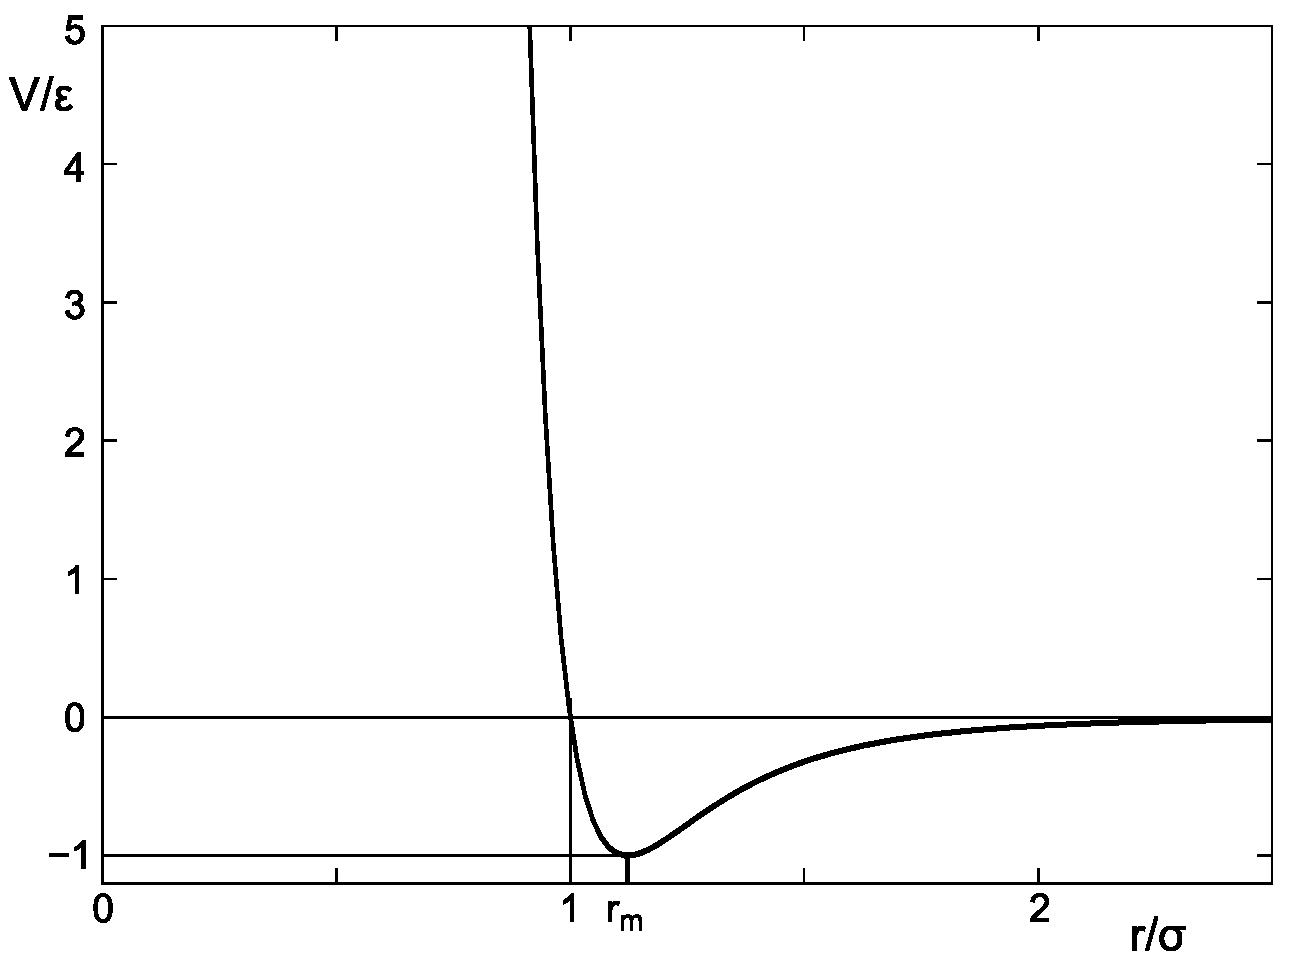
\includegraphics[width=0.7\textwidth]{template_files/LJ} 
  \caption{The Lennard--Jones potential.
  Make sure you label and have units on all axes! Also make sure that labels etc.\
  are legible and that, if you print in black and white, that you use different line
  styles when required to differentiate between curves. In \textsc{matlab}
  you can export any figure to an .eps file from File $\rightarrow$
  Export\ldots\ in the Figure window.}
  \label{fig1}
\end{center}
\end{figure}
  
\section*{Problem 2}

In the following we give an example of how to produce a table.
Use the code for Table~\ref{tab1} as a template.

\begin{table}[!ht]
  \begin{center}
    \caption{A dummy table}
    \begin{tabular}{l|c|c}\hline\hline
      \textbf{Col.~1} & \textbf{Col.~2} & \textbf{Col.~3} \\ \hline
      the & quick & brown \\ 
      fox & jumps & over \\ 
      the & lazy  & dog \\ 
      \hline\hline
    \end{tabular}
    \label{tab1}
  \end{center}
\end{table}

\section*{Problem 3}

If you find some part of the code particularly interesting you may 
include it in the text, otherwise it should be included in the appedix.
If you do want to include code the following commands will print
the text directly, with no \LaTeX~commands executed:

\begin{lstlisting}[language=matlab]
% Hello world ten times in MATLAB
for i = 1 : 10
  fprintf('Hello world %d!\n',i);
end
\end{lstlisting}

\begin{lstlisting}[language=python]
# Hello world ten times in Python
for i in range(10):
  print 'Hello world %d!' % i
\end{lstlisting}

\section*{Problem 4}
At some point it may be appropriate to include equations. It is done in the
following way:

\begin{equation}
  V(r) = 4\epsilon \left[ \left( \frac{\sigma}{r} \right)^{12} - 
    \left(\frac{\sigma}{r} \right)^{6} \right]
\end{equation}

Do number and reference all your equations.

\section*{Concluding discussion}

Use your favourite flavor of \LaTeX{} to compile the file:
\begin{verbatim}
xelatex template.tex
pdflatex template.tex
latex template.tex
\end{verbatim}
should all work.
If you use \verb+pdflatex+ or \verb+xelatex+, included figures need to be in
\verb+pdf+, \verb+jpg+, or \verb+png+ format. If you want to include eps
figures, you can easily convert them to \verb+pdf+ using the command
\begin{verbatim}
ps2pdf -dEPSCrop figure.eps figure.pdf
\end{verbatim}

\begin{thebibliography}{69}
\bibitem{lamport94} Leslie Lamport, \emph{\LaTeX: A Document Preparation
System}. Addison Wesley, Massachusetts, 2nd Edition, 1994.
\end{thebibliography}

\newpage

\appendix

\section{Source Code}

Include all source code here in the appendix. Keep the code formatting clean,
use indentation, and comment your code to make it easy to understand. Also,
break lines that are too long. (Keep them under 80 characters!)

\subsection{Calculating pi using matlab: \texttt{pi.m}}
\lstinputlisting[language=matlab,numbers=left]{template_files/pi.m}

\subsection{Calculating pi using python: \texttt{pi.py}}
\lstinputlisting[language=python,numbers=left]{template_files/pi.py}

\subsection{Calculating pi using C: \texttt{pi.c}}
\lstinputlisting[language=c,numbers=left]{template_files/pi.c}

\end{document}
